
\chapter{Failsafe Mechanism Design using State Tree Structures}

Autonomous Aerial Refueling (AAR) is vulnerable to various failures and involves cooperation among autonomous receivers, tankers and remote pilots. Dangerous flight maneuvers may be executed when unexpected failures or command conflicts happen. To solve this problem, a failsafe mechanism based on State Tree Structures (STS) is proposed. The failsafe mechanism is a control logic that guides what subsequent actions the autonomous receiver should take, by observing real-time information of internal low-level subsystems such as guidance and drogue\&probe and external instructions from tankers and pilots. To generate such a controller using STS, the AAR procedure is decomposed into several modes, and safety issues related with seven low-level subsystems are summarized. Then common functional demands and safety requirements are textually described. On this basis, the AAR plants and specifications are modeled by STS, and a supervisor is synthesized to control the AAR model. To prove its feasibility and correctness, a simulation environment incorporating such a logic supervisor is built and tested. The design procedures presented in this paper can be used in decision-making strategies for similar flight tasks. Supporting materials can be downloaded in \href{https://github.com/KevinDong0810/Failsafe-Design-for-AAR-using-STS}{Github}\footnote{https://github.com/KevinDong0810/Failsafe-Design-for-AAR-using-STS}, including related software, input documents and output files.

\section{Introduction}
%	\linenumbers
Autonomous Aerial Refueling (AAR) is an effective approach to increase the range and endurance of Unmanned Aerial Vehicles (UAV) by refueling them in air. Since the first successful AAR concept demonstration by the Boeing company, several ambitious AAR projects have been carried on by the NASA \cite{dibley2007autonomous}, US Air Force and US Navy \cite{THOMAS201414}, which demonstrate the feasibility and reliability of AAR. During an AAR operation, as shown in Fig. \ref{fig:AAR_simple}, a UAV (or a receiver) detaches from its formation and approaches the rear of a tanker for refueling. Once refueled and cleared, the receiver disengages from the tanker and rejoins the formation. The boom system or drogue\&probe system is used for fuel transfer, and this paper focuses on the drogue\&probe system, as shown in Fig. \ref{fig:drogueprobe}, for the drogue\&probe's advantages for autonomous systems. \cite{bolkcom2006air, dibley2007autonomous}	
\begin{figure}[H]
	\begin{minipage}[t]{0.5\textwidth}
		\centering
		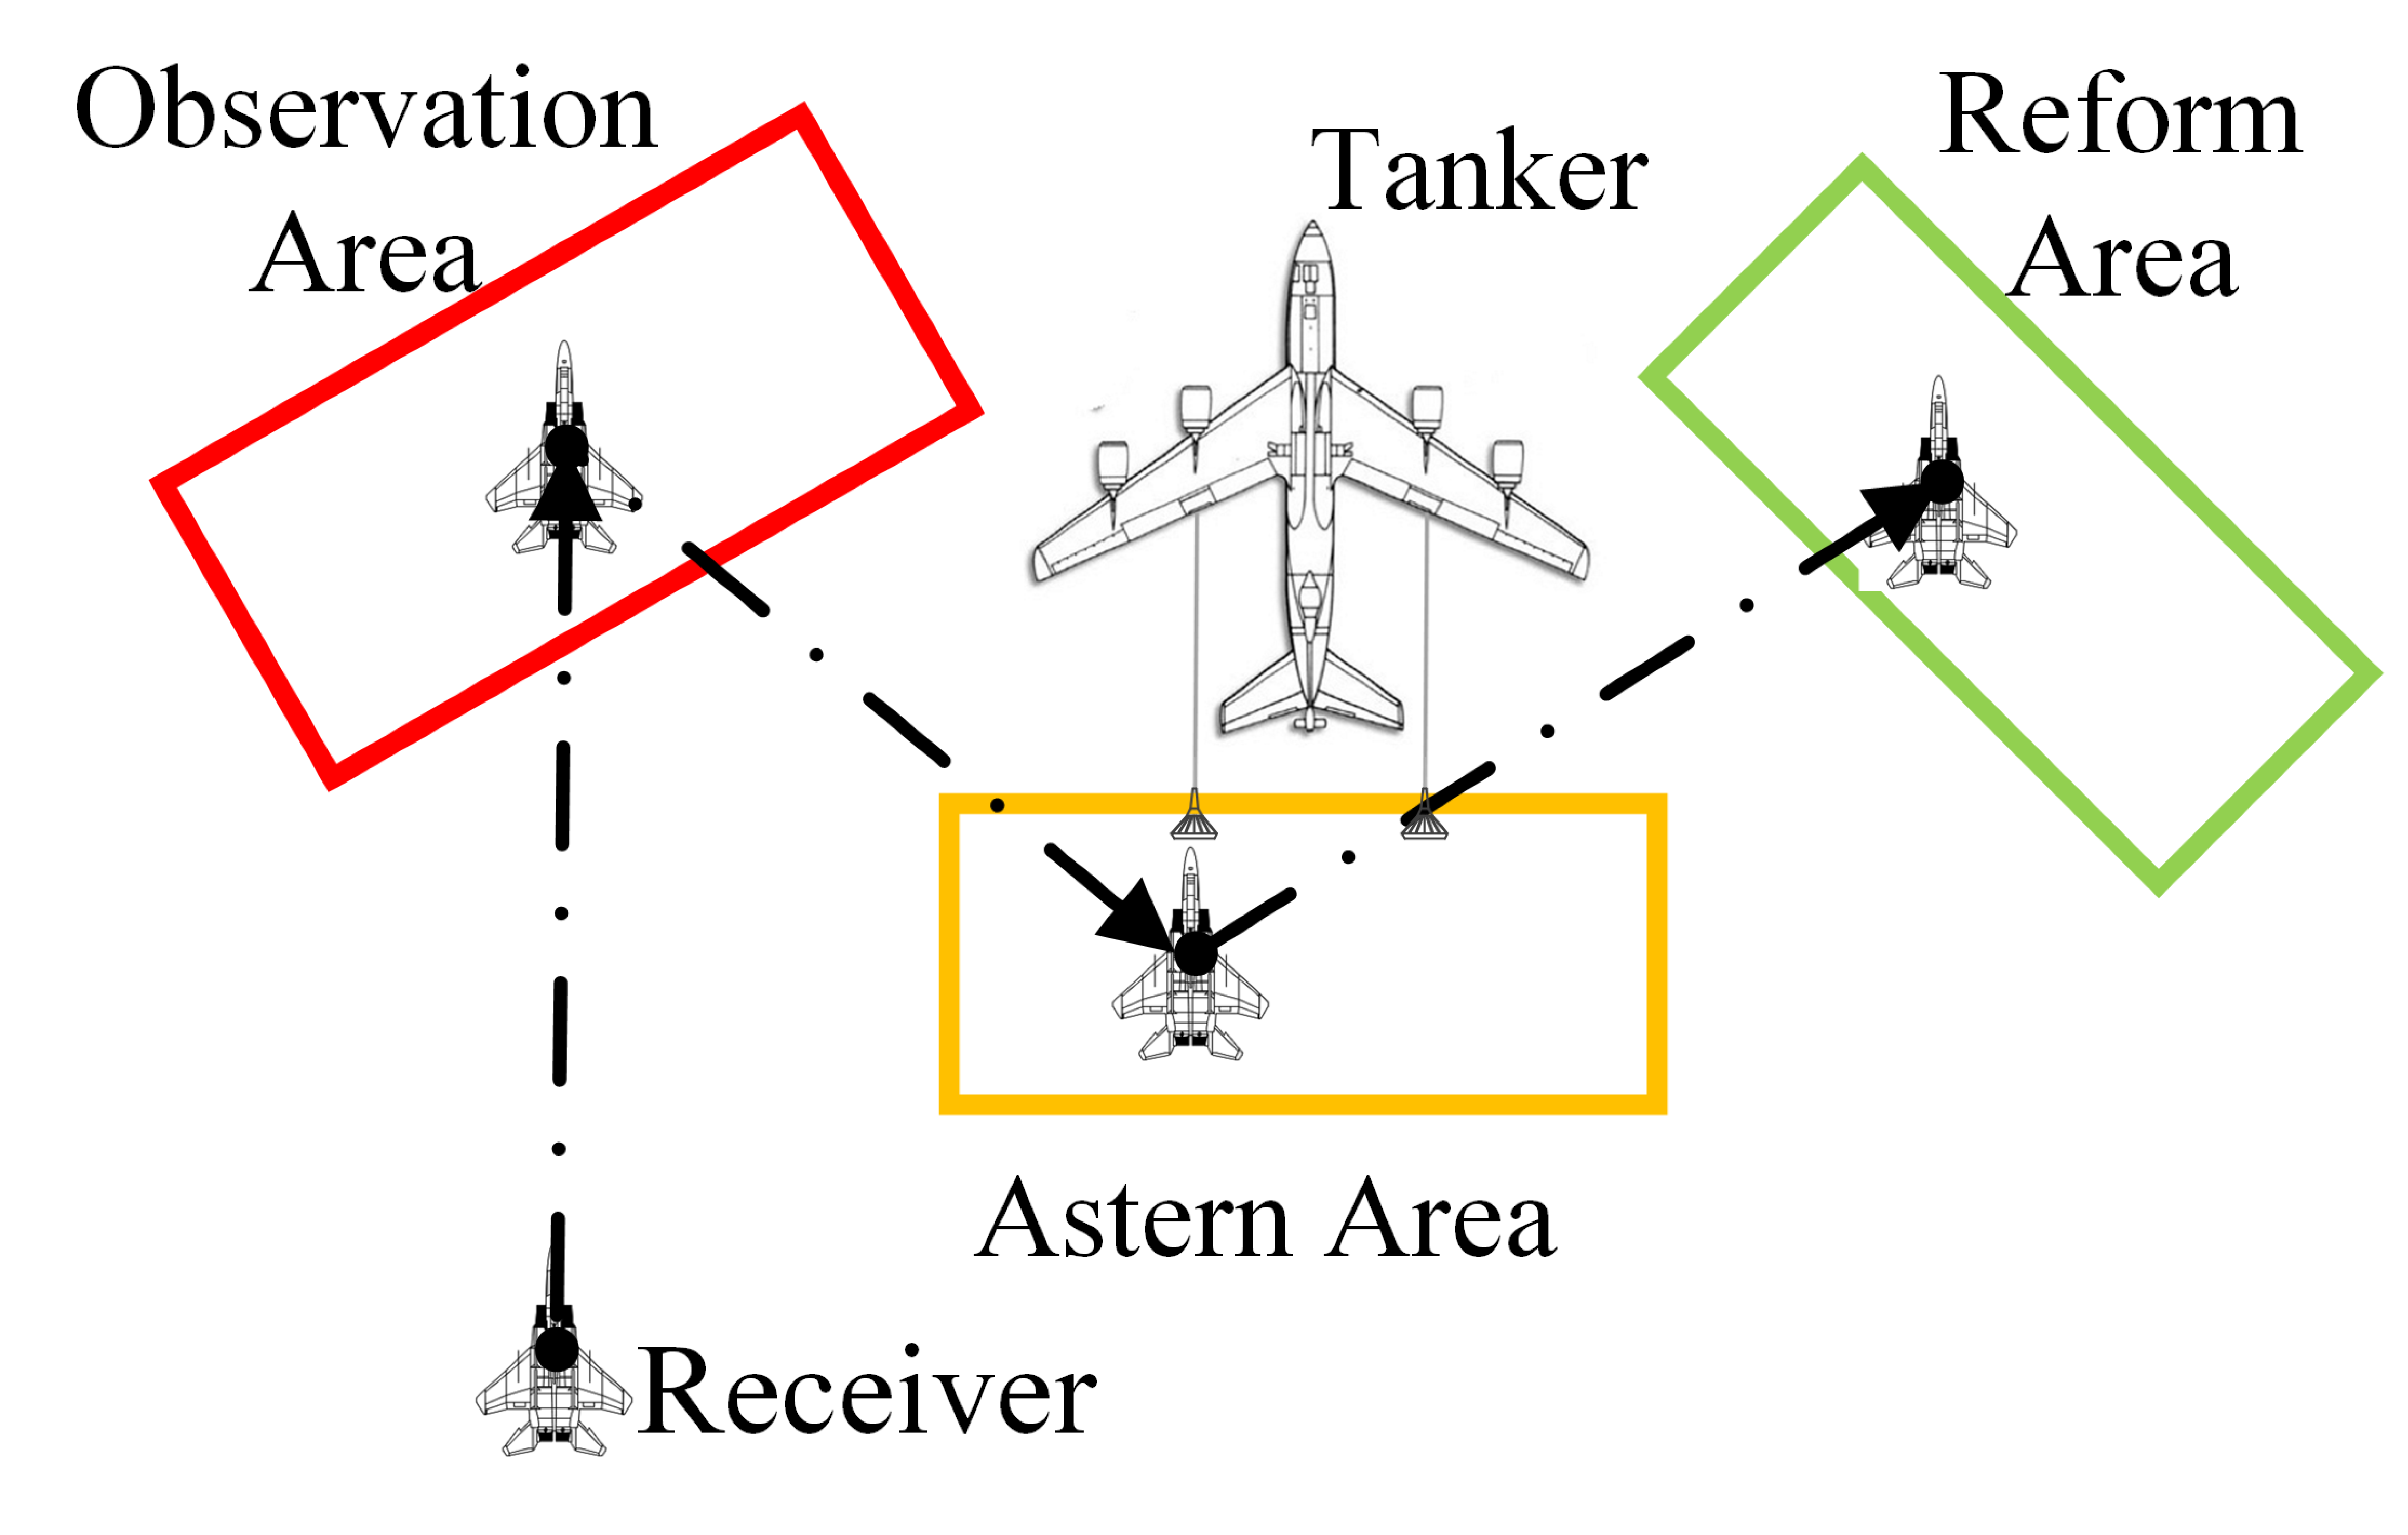
\includegraphics[scale=0.08]{Figures/Figs_Ch14/Fig1a_simpleAAR}
		\caption{JOINING-INIT MODE.\label{fig:AAR_simple}}
	\end{minipage}
	\qquad
	\begin{minipage}[t]{0.5\textwidth}
		\centering
		\includegraphics[scale=0.05]{Figures/Figs_Ch14/Fig1b_DrogueProbe}
		\caption{JOINING-WAIT MODE.\label{fig:drogueprobe}}
	\end{minipage}
	\label{Fig:joining}
\end{figure}

The AAR is a semi-automated process, where the control of unmanned receivers relies on frequent interactions among the on-board receiver controller, external tanker controller and remote human pilots. Therefore, command conflicts may happen and jeopardize the refueling task.  Besides, an AAR process is vulnerable to various system failures like probe damage and unsteady airflow. Therefore, a high-level logic controller that coordinates all these control components and produces the desired safe functionality in the presence of faults and failures is needed, namely a \textit{failsafe mechanism}. A wealth of researches have been done in this domain. Ref [\citen{degani2002formal}] formalized the general framework for formal verification of human-automaton interface, where both automaton and human controller share the authority over the system. Refs [\citen{mitchell2005time}] and [\citen{ ding1770reachability}] investigated the safe path planning in AAR to avoid collision with consideration of receiver-pilot interaction. In the Research Flight Control System developed by  [\citen{dibley2007autonomous}] in NASA, human-machine interface is put into practice. But none of them has taken system failures into consideration for logic design, under which dangerous maneuvers may happen. In contrast, fault-related literature is  mainly focused on low-level controllers, such as fault detection techniques \cite{meskin2010hybrid} and fault-tolerant control algorithms \cite{zhang2006issues, falconi2016adaptive}. As far as the authors know, no high-level logic controller has been studied.

At present, the failsafe mechanism design for AAR is seldom investigated. Related applications like rotorcrafts mainly count on engineering experience and manual calculation to design the control logic, like DJI autopilot and ArduPilot autopilot. Man-made mistakes, logical bugs or an incomplete treatment are hard to avoid in this approach. And when it comes to complex systems, this approach is very time-consuming. Therefore, this paper aims to use a model-based method, namely supervisory control theory (SCT) of state tree structures (STS), to design a comprehensive failsafe mechanism.

SCT is a formal method for synthesizing supervisors of discrete-event systems. On observing event strings generated by the plant, at each state the SCT would disable a suitable subset of controllable events to satisfy the given control specifications \cite{WONHAM20171791}. First put forward by [\citen{Ramadge21072}], the SCT has a sound theoretical foundation \cite{cai2010supervisor, wonham2015supervisory}, and numerous industrial applications such as testbed assembly process \cite{brandin1994},  telephone directory assistance call center \cite{seidl2006} and magnetic resonance image (MRI) scanner \cite{theunissen2014}. Later, to solve the problem of exponential computational effort faced by finite state machine (FSM) used in original SCT, \textit{state charts} \cite{HAREL1987231} are adopted and this new version of SCT is named STS \cite{ma2006nonblocking}.  The STS uses the AND (Cartesian product) and OR (disjoint union) operation to present system hierarchies and uses \textit{binary decision diagrams} (BDD) \cite{Bryant86} to manage the computational complexity. 

Compared with current failsafe mechanisms based on engineering experience, the STS approach has three main advantages: 1) \textit{Correct by design}: The restricted behaviors under the supervision of the STS ensure that requirements are satisfied. Therefore, the control logic is free from incomplete treatment and logical bugs in the design phase. 2) \textit{Compact}: The resulting supervisor is presented in the simplest way, which means when making a decision, only necessary information instead of the whole system state would be required. Therefore, a minimal disabling action is made for the system to stay within safe states. 3) \textit{Flexibility}: The STS allows the modular modeling method and ensures the system can be readily evolved. Different modules (subsystems, requirements, etc.) can be added easily when taking different control hierarchies (from high-level to low-level) into consideration. This has been well presented in the application of theme park vehicles \cite{Forschelen2012Application}.

The main contributions of this paper are the following: 
\begin{itemize}
	\item This paper  investigates the failsafe logic design of autonomous receivers using a sound formal verification theory. A supervisor is synthesized to cover common system failures and interaction among receivers, tankers and pilots. This design framework can be easily adopted for different aerial refueling procedures and other similar control tasks.
	\item Tools for synthesizing, implementing and simulating supervisors gained through STS for aerial refueling have been developed and posted in Github. This may stimulate the similar failsafe mechanism design in related domains.
\end{itemize}

The remainder of this paper is organized as follows. Section 2 summarizes the basics of STS. Section 3 presents the discretization of AAR procedures and summary of common safety issues. In section 4, functional demands and safety requirements are provided, as well as the event definitions. On this basis, section 5 presents the STS design of AAR and the generated supervisor using related software. In section 6, the supervisor is implemented in a simulation environment for AAR and tested for correctness. Section 7 concludes this paper.

\section {Preliminaries of STS}
This section presents the basics of STS theory, while details can be found in textbooks \cite{ma2006nonblocking, cai2010supervisor, wonham2015supervisory}. 

\subsection{State Tree Structure}
\label{sec:sts}
The State tree structure is an extension of the finite state machine in SCT, which introduces natural hierarchical structures into the system model. It mainly consists of two parts: \textit{state tree} and \textit{holon}. These two parts depict the same system but focus on different aspects. State tree, say \textbf{ST}, organizes the state space of an STS, while the holon, say \textbf{H}, organizes the transitions of an STS. The nodes on a state tree are called states. Every state tree has a unique root state. A state on a state tree is called an OR (resp. AND) \textit{superstate} if it can be represented as the disjoint union $\rm \dot U $ (resp. Cartesian product $\rm X $) of its children. Each child state is called an OR (resp. AND) superstate. The lowest level states are called \textit{simple states}, which are required to be OR superstates to avoid redundant information. In the following text, the states of STS including simple states and superstates, are written in italics and start with capitals like \textit{Standby}. In most application scenarios, OR superstates work sequentially while AND superstates work concurrently. 


\textit{Holon} organizes the state transitions of STS, which can be regarded as an automaton with hierarchies. It depicts the boundary and local state transitions of the state tree. A holon $ \mathbf{H}$ is a 5-tuple $ \mathbf{H}:=\{ {X},{\varSigma},{\delta},X_{\rm{o}},X_{\rm{m}} \} $, where $ X $ is a finite set consisting of states in \textbf{ST}; $ \varSigma $ is the finite event set (also called an \textit{alphabet}); $ \delta $ is the (partial) transition function on the state set: $ \delta:X \times\Sigma \to X $ ; $ X_{\rm{o}} \subseteq X$ is a subset of $ X $ consisting of \textit{initial states}; $ X_{\rm{m}} \subseteq X $ is another subset of $ X $ consisting of \textit{marker states} that the whole system desires to reach. 

In SCT, the alphabet $ \varSigma $ is partitioned as $  \varSigma  = {\varSigma_{\rm{c}}} \cup {\varSigma _{\rm{u}}}$, where $ \varSigma _{\rm{c}} $ is the subset of \textit{controllable events} that can be disabled at will while $ \varSigma _{\rm{u}} $ is the subset of \textit{uncontrollable events} that cannot be disabled by the controller. In engineering practice, $ \varSigma _{\rm{c}} $ usually represents relevant discrete commands to the low-level controller, while  $ \varSigma _{\rm{u}} $ usually represents messages sent to the supervisor such as system health information and sensor signals like the waiting time exceeding a pre-defined threshold.

\subsection{Plant, Specification and Supervisor}
\label{sec:pss}
SCT aims to synthesize the supremal non-blocking language (event sequences) of \textit{Plant}, while satisfying the requirements of \textit{Specification}. The generated language is called \textit{Supervisor}; their detailed descriptions are given as follows.
\begin{itemize}
	\item \textbf{Plant}. Plants are models of behaviors of physical systems and processes, which contain all the possible states and transitions. 
	\item \textbf{Specification}. Specifications are models of control requirements, which point out the unwanted states and transitions in correspondence to forbidden states. It can be given as illegal state sets\cite{Markovski2010Coordination} or illegal event sequences\cite{Forschelen2012Application}. The latter form is used in this paper.
	\item \textbf{Supervisor}. The supervisor is the minimally restrictive event sequence of plants under the restriction of specifications, and is implemented by state feedback control functions \cite{ma2006nonblocking} for events. In every state of the plant, the supervisor will provide a subset of controllable events among which the plant can choose one to execute. By doing so, the specifications are always satisfied.
\end{itemize}

In the synchronization algorithm, namely \textit{Supcon}, for supervisors \cite{ma2006nonblocking}, all uncontrollable event sequences leading to \textit{blocking states}, namely states that cannot reach marker states by any event transitions, are deleted iteratively. Therefore, to model the specifications, the undesired event sequence should be made to lead to blocking states. \footnote{Readers can find a similar example in Exercise 3 of Chapter 3.10 in the DES textbook \cite{wonham2015supervisory} for a better understanding.}

\section{Mode Discretization and Safety Issues}
\label{sec:mode}
This section describes the plant for aerial refueling. Related AAR procedures are discretized and common safety issues are summarized, according to which the STS plant will be modeled. 

\subsection{Area Definition}
The procedure discretization is based on air space decomposition. The air space is divided into different areas according to their locations relative to the tanker.
\begin{figure}[h]
	\begin{center}
		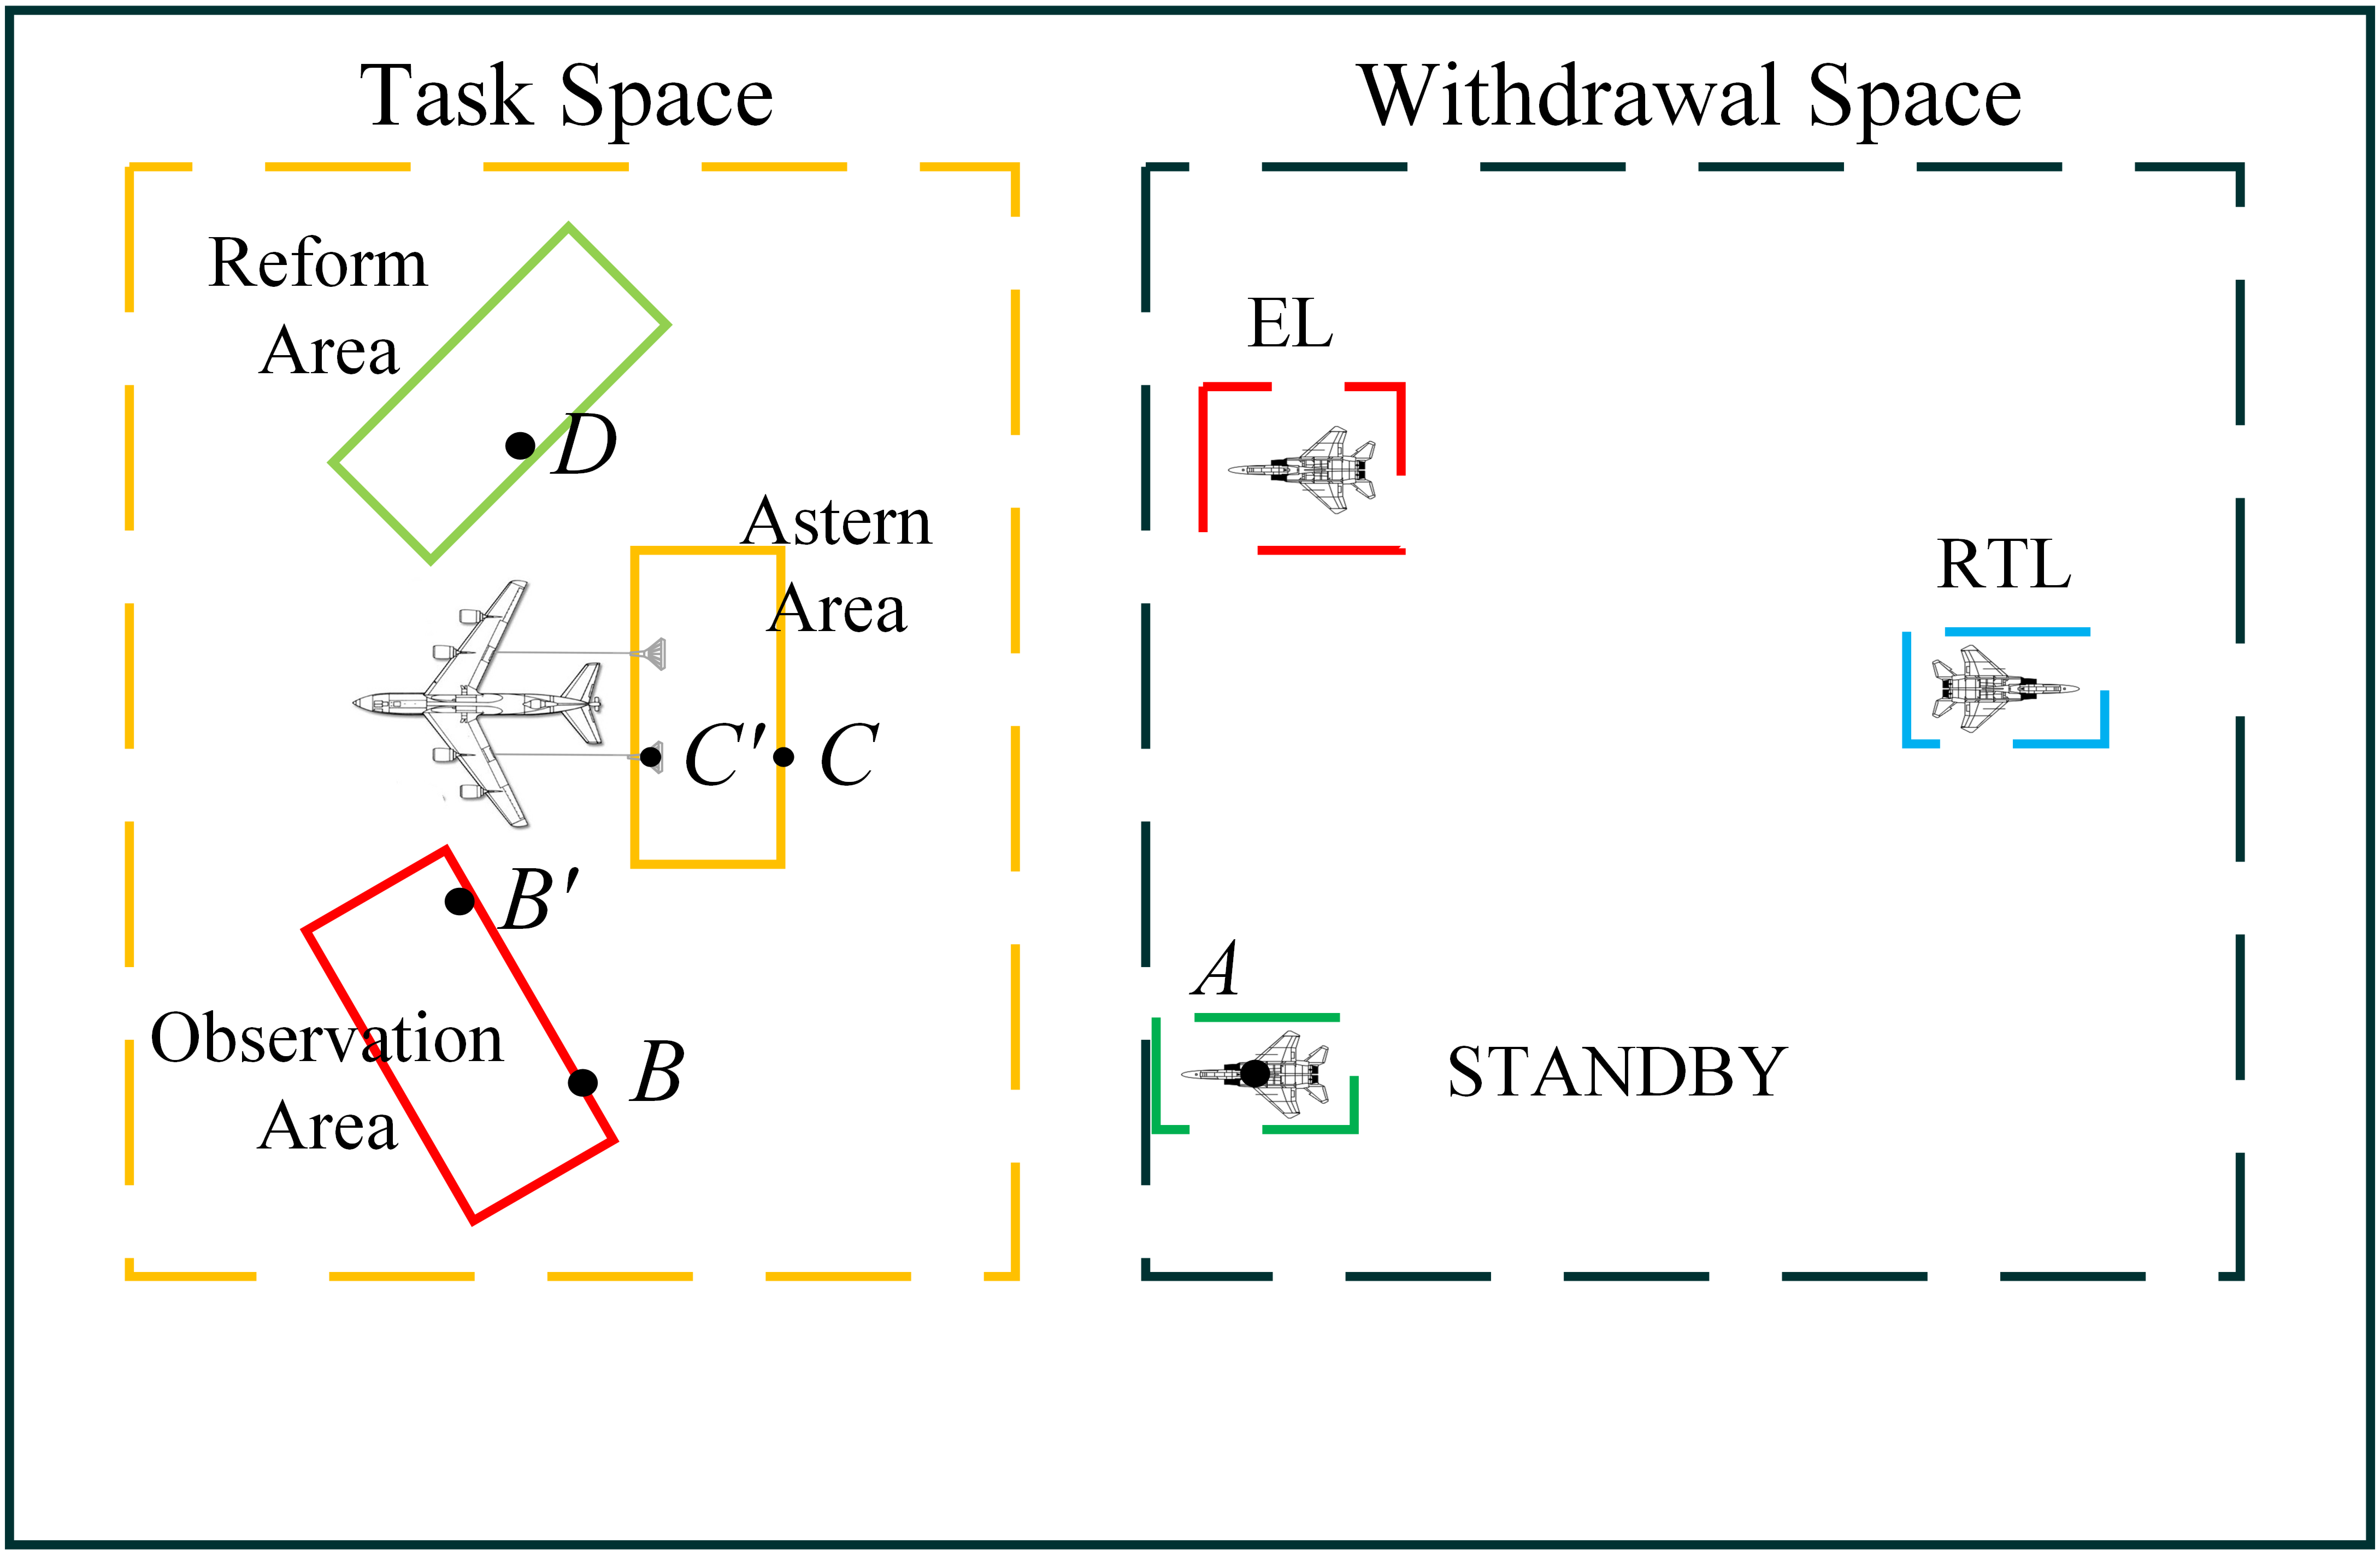
\includegraphics[width=0.5\textwidth]{Figures/Figs_Ch14/Fig5_AreaView_Top}
		\par\end{center}
	\caption{Top view of the air space division}
	\label{fig:topview} 
\end{figure}
\begin{figure}[h]
	\begin{center}
		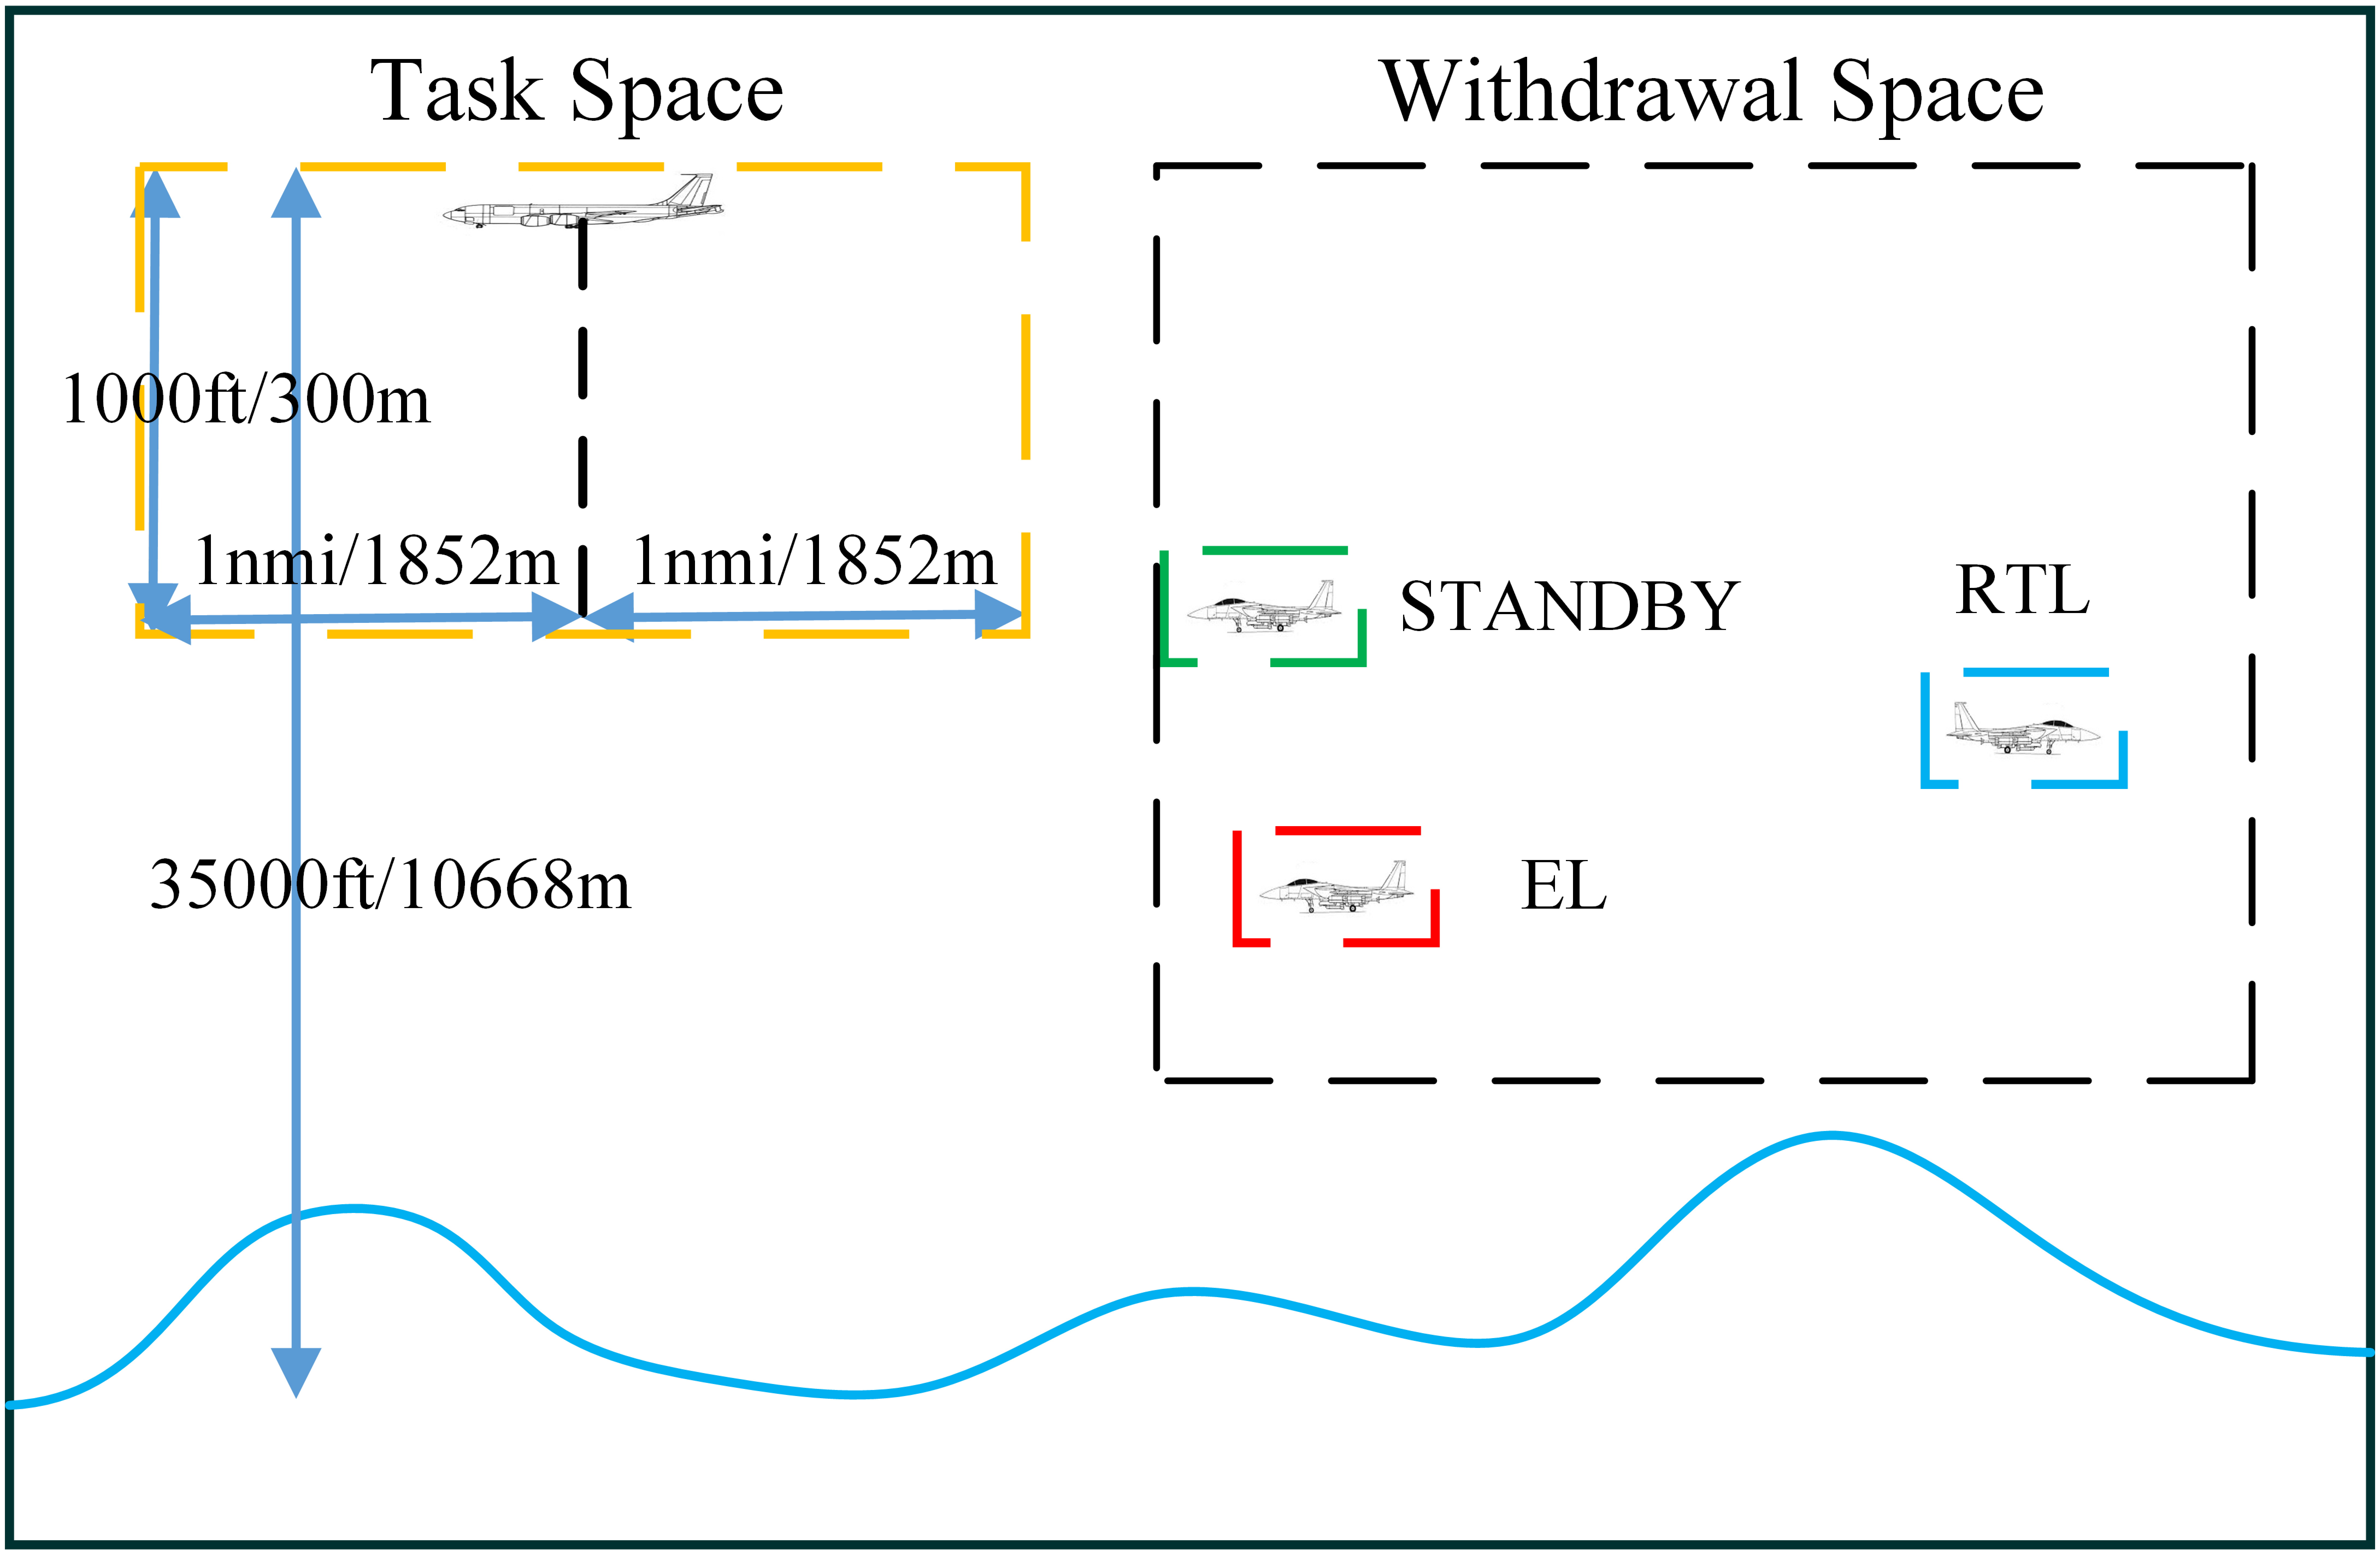
\includegraphics[width=0.5\textwidth]{Figures/Figs_Ch14/Fig5_AreaView_Side}
		\par\end{center}
	\caption{Top view of the air space division}
	\label{fig:sideview} 
\end{figure}

As shown in Fig. \ref{fig:topview} and \ref{fig:sideview}, the air space is divided into two parts: \textit{Task Space} and \textit{Withdrawal Space}. The task space is the space where AAR tasks are carried out. It is assumed to be a box space centered at the tanker with 300m height(downward), 3704m length and an appropriate width.\footnote{These data are given according to \cite[p.~54]{NATO2010} that the refueling start point should be placed 1000ft(300m) below and 1nmi (1852m) behind the tanker.} The task space contains three areas: observation area, astern area and reform area. The observation area at the left-hand side of the tanker is allocated for joining receivers. The astern area is the stabilized formation position behind the AAR equipment, approximately 100ft-aft of the drogue directly \cite[p.~32]{NATO2010}. The reform area is the area at the right and level or slightly above the tanker formation.

The withdrawal space is the airspace outside of the task space used for emergency and AAR preparation. When AAR is achieved or failed, the receiver will enter into the withdrawal space from the task space. On the other hand, when the receiver's health conditions allow a possible AAR, the receiver will enter the task space from the withdrawal space. The withdrawal space has three maneuver modes including STANDBY, RTL and EL, whose definitions are presented in section \ref{sec:withdrawphase}.

\subsection{Mode Decomposition}
\label{sec:mode_decom}

Based on the air-to-air refueling demonstration of [\citen{dibley2007autonomous}] and standard  procedures for manned aircraft proposed by [\citen{NATO2010}], the AAR work cycle is decomposed into the following distinct phases and modes. In the following text, the AAR mode will be presented in capitals like STANDBY MODE.\footnote{Standby can be a mode like STANDBY MODE or a simple state like \textit{Standby}. They are two different concepts in this paper, but refer to the same thing in the physical world.}

\subsubsection{Withdrawal Phase}
\label{sec:withdrawphase}
The withdrawal phase is in correspondence to the withdrawal space. As mentioned before, there are three modes in this phase or space, namely STANDBY, RTL and EL. 

\vspace{1ex}
\hspace{-1.5em}\textbf{a) STANDBY MODE:} The receiver is waiting at point $ A $ (as shown in Fig. \ref{fig:topview}) for the next instruction. In this mode, the receiver has the ability to carry on AAR tasks.

\vspace{1ex}
\hspace{-1.5em}\textbf{b) Return to Land (RTL) MODE:} The receiver returns to the nearest airbase to land, which may result from subsystem failures or pilot instructions. In this mode, the receiver may lose the ability to carry on AAR tasks but still keep the ability to return to base.

\vspace{1ex}
\hspace{-1.5em}\textbf{c) Emergency Landing(EL) MODE:} The receiver makes an emergency landing, which may result from subsystem failures or pilot instructions. In this mode, the receiver may lose the ability to return to base and can only make an emergency landing.

\subsubsection{Task Phase}
The task phase contains all the AAR task procedures, mainly the joining, refueling and reforming sub-phases.

\vspace{1ex}
\hspace{-1.5em}\textbf{a) Joining Sub-Phase:} Joining refers to the sub-phase where the receiver maneuvers from STANDBY MODE to the observation area. It has two modes:

%\begin{verbatim}
\begin{enumerate}
	\item \textbf{JOINING-INIT MODE}: As shown in Fig. \ref{Fig:joining}\subref{fig:joininit}, the receiver flies to the observation area. The control objective is to control the receiver flying from STANDBY MODE to point $ B $.
	\item \textbf{JOINING-WAIT MODE}: As shown in Fig. \ref{Fig:joining}\subref{fig:joinwait}, the receiver stays in the observation area and waits for the \textit{connection clearance} from the tanker, namely the command given by the tanker to allow the receiver to fly to the astern area and connect its probe with the drogue. The control objective is to control the receiver flying to point $ B' $ and then keep the position.
\end{enumerate}

\hspace{-1.5em}\textbf{b) Refueling Sub-Phase:} Refueling refers to the sub-phase where the receiver connects to the tanker and transfers the fuel. It has three modes. 
\begin{enumerate}
	\item \textbf{REFUELING-INIT MODE}: As shown in Fig. \ref{Fig:refueling}\subref{fig:refuelinginit}, once the receiver is cleared for the connection it flies to the astern area. The control objective is to control the receiver flight to point $ C $ and then maintain the position.
	\item \textbf{REFUELING-CAPTURE MODE}: The receiver initiates the connection between the probe and the tanker's drogue. As shown in Fig. \ref{Fig:refueling}\subref{fig:refuelingcap}, the control objective is to control the receiver flying to point $ C' $, and then keep the position for connecting the probe with the drogue.
	\item \textbf{REFUELING-TRANSFER MODE}: After a successful capture, the receiver and the tanker keep relatively stationary to transfer the fuel. When the fuel transfer is finished, the receiver should still keep connected with the tanker and wait for the \textit{disconnection clearance}, namely the command given by the tanker to allow the receiver to disconnect from the drogue. As shown in Fig. \ref{Fig:refueling}\subref{fig:refuelingtran}, the control objective is to keep the receiver at the point  $ C' $ and transfer the fuel.
\end{enumerate}

\begin{figure}[h]
	\centering
	\subfloat[JOINING-INIT MODE]{\label{fig:joininit}
		
\includegraphics[scale=0.035]{Figures/Figs_Ch14/Fig6a_Joining_Init}}\qquad
	\subfloat[JOINING-WAIT MODE]{\label{fig:joinwait}
		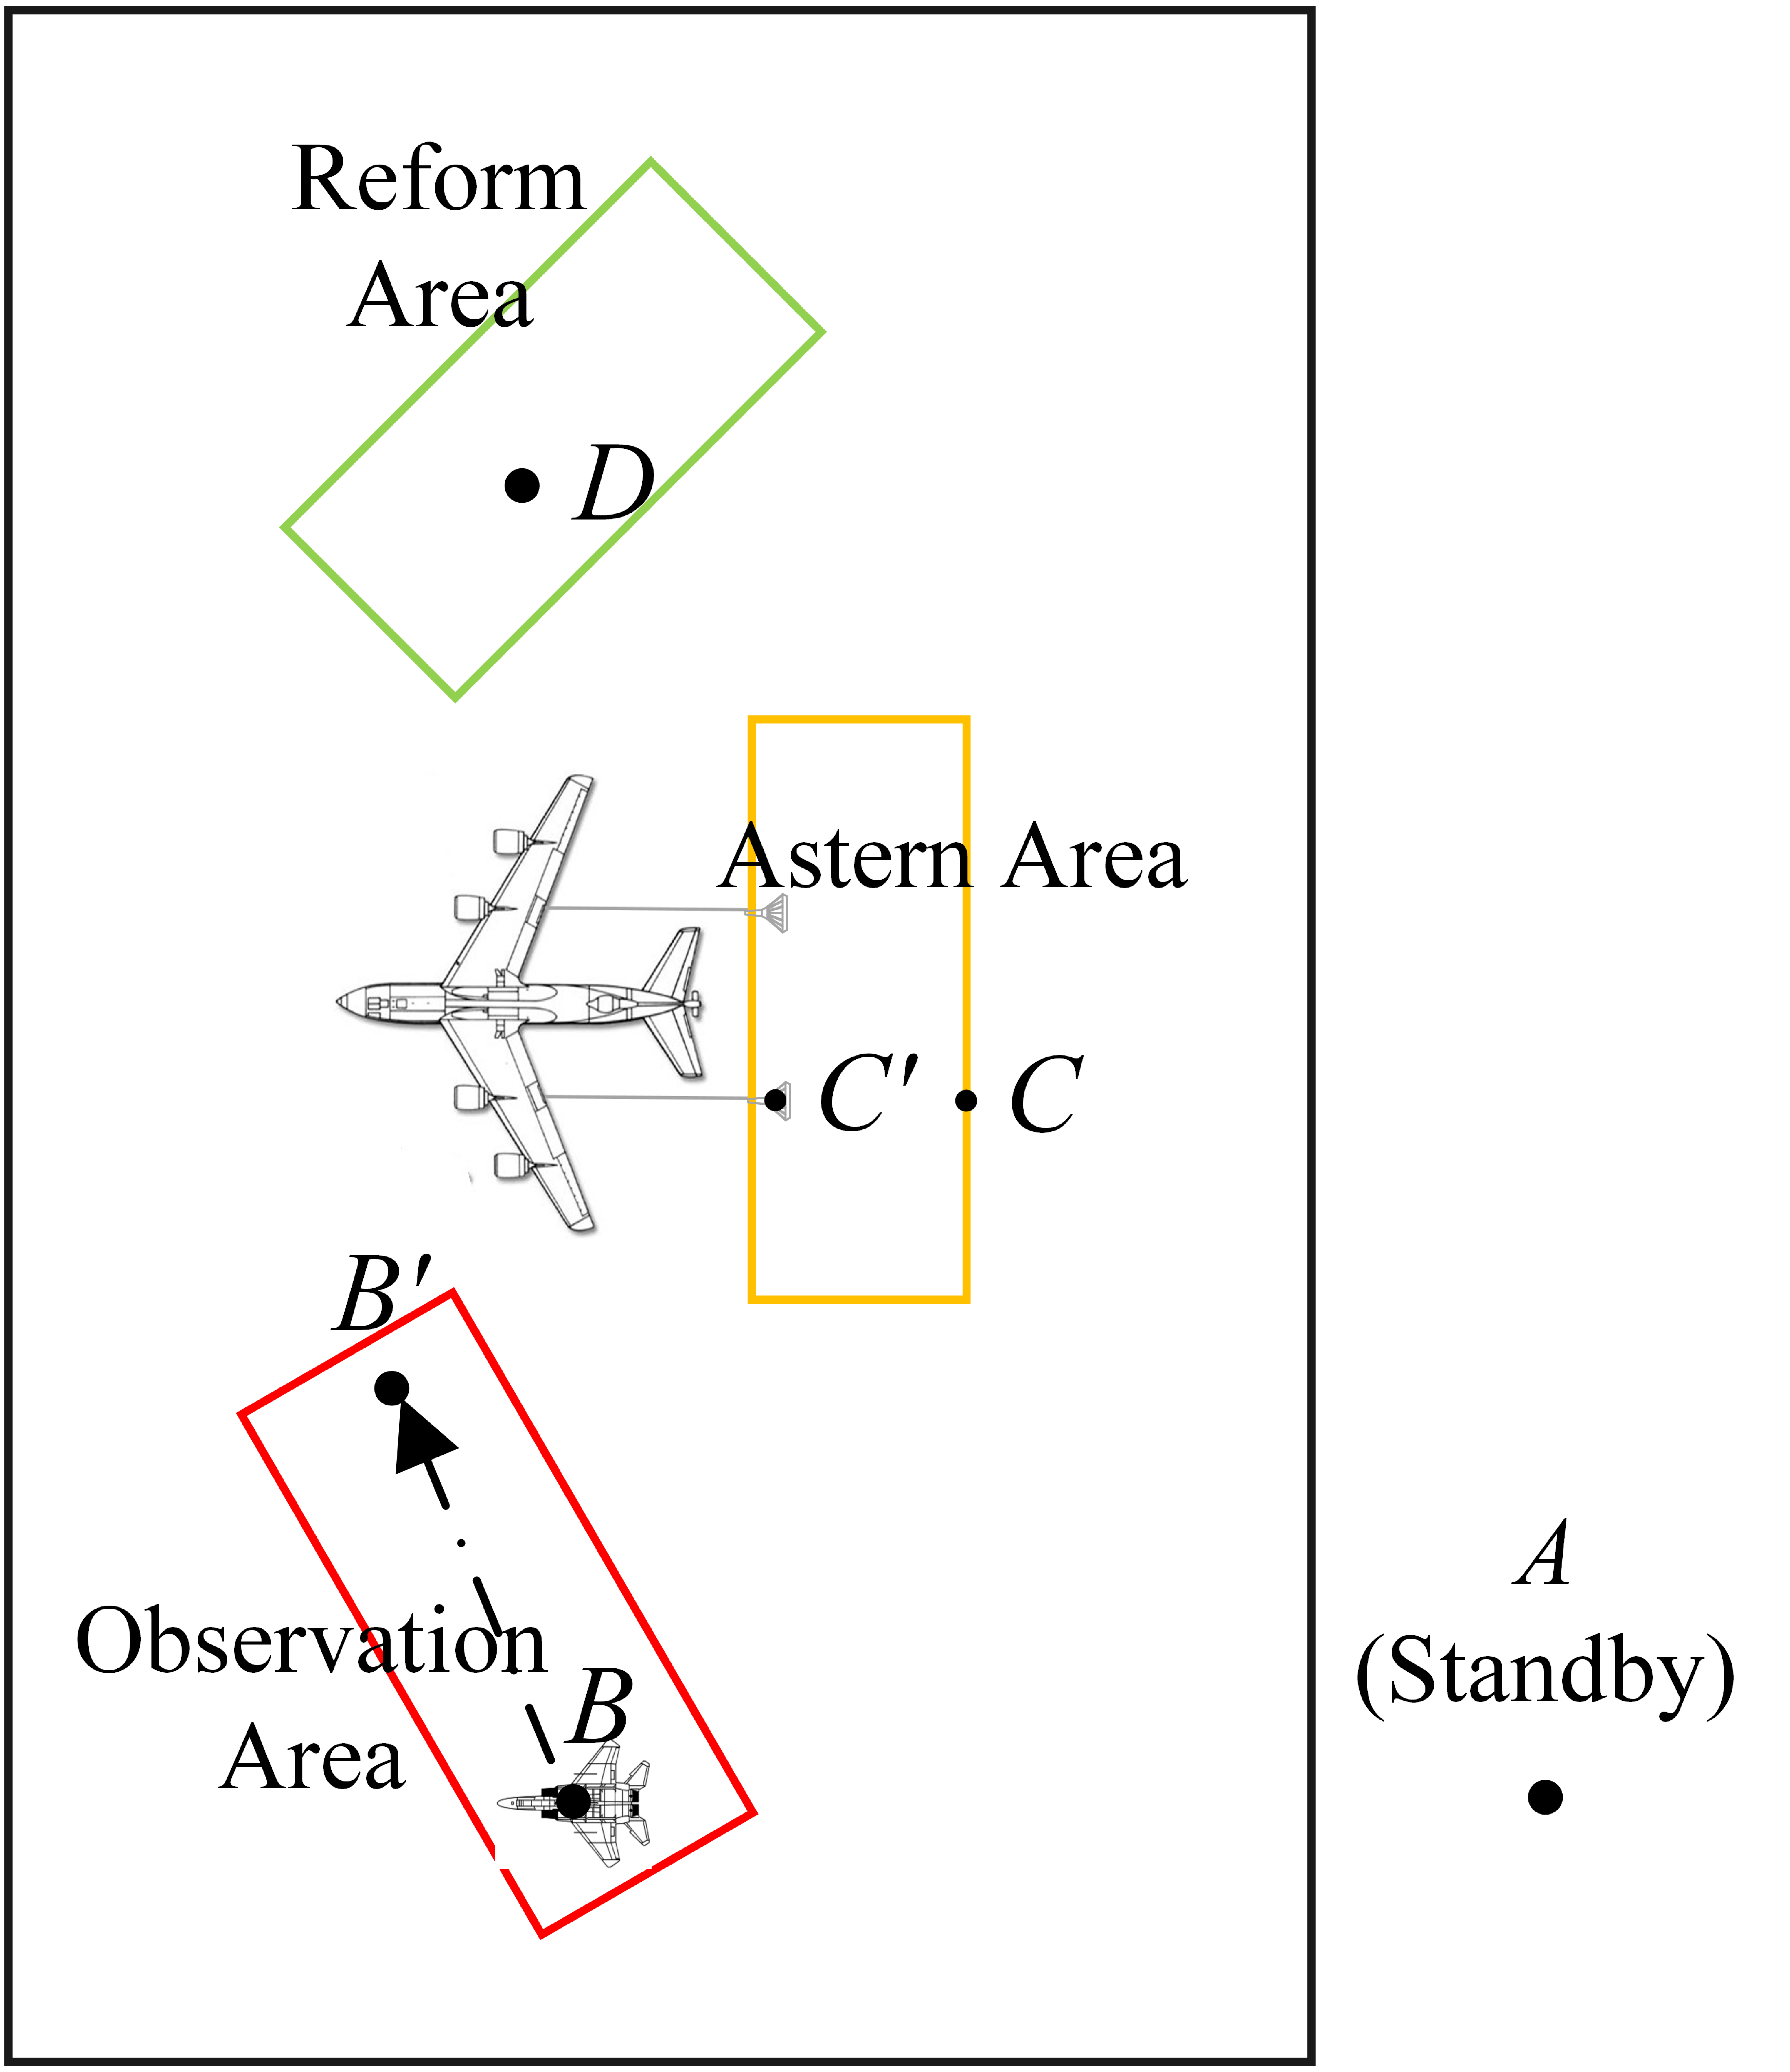
\includegraphics[scale=0.035]{Figures/Figs_Ch14/Fig6b_Joining_Wait}}
	\caption{Joining sub-phase.}
	\label{Fig:joining}
\end{figure}




\begin{figure}[h]
	\centering
	\subfloat[REFUELING-INIT MODE]{\label{fig:refuelinginit}
		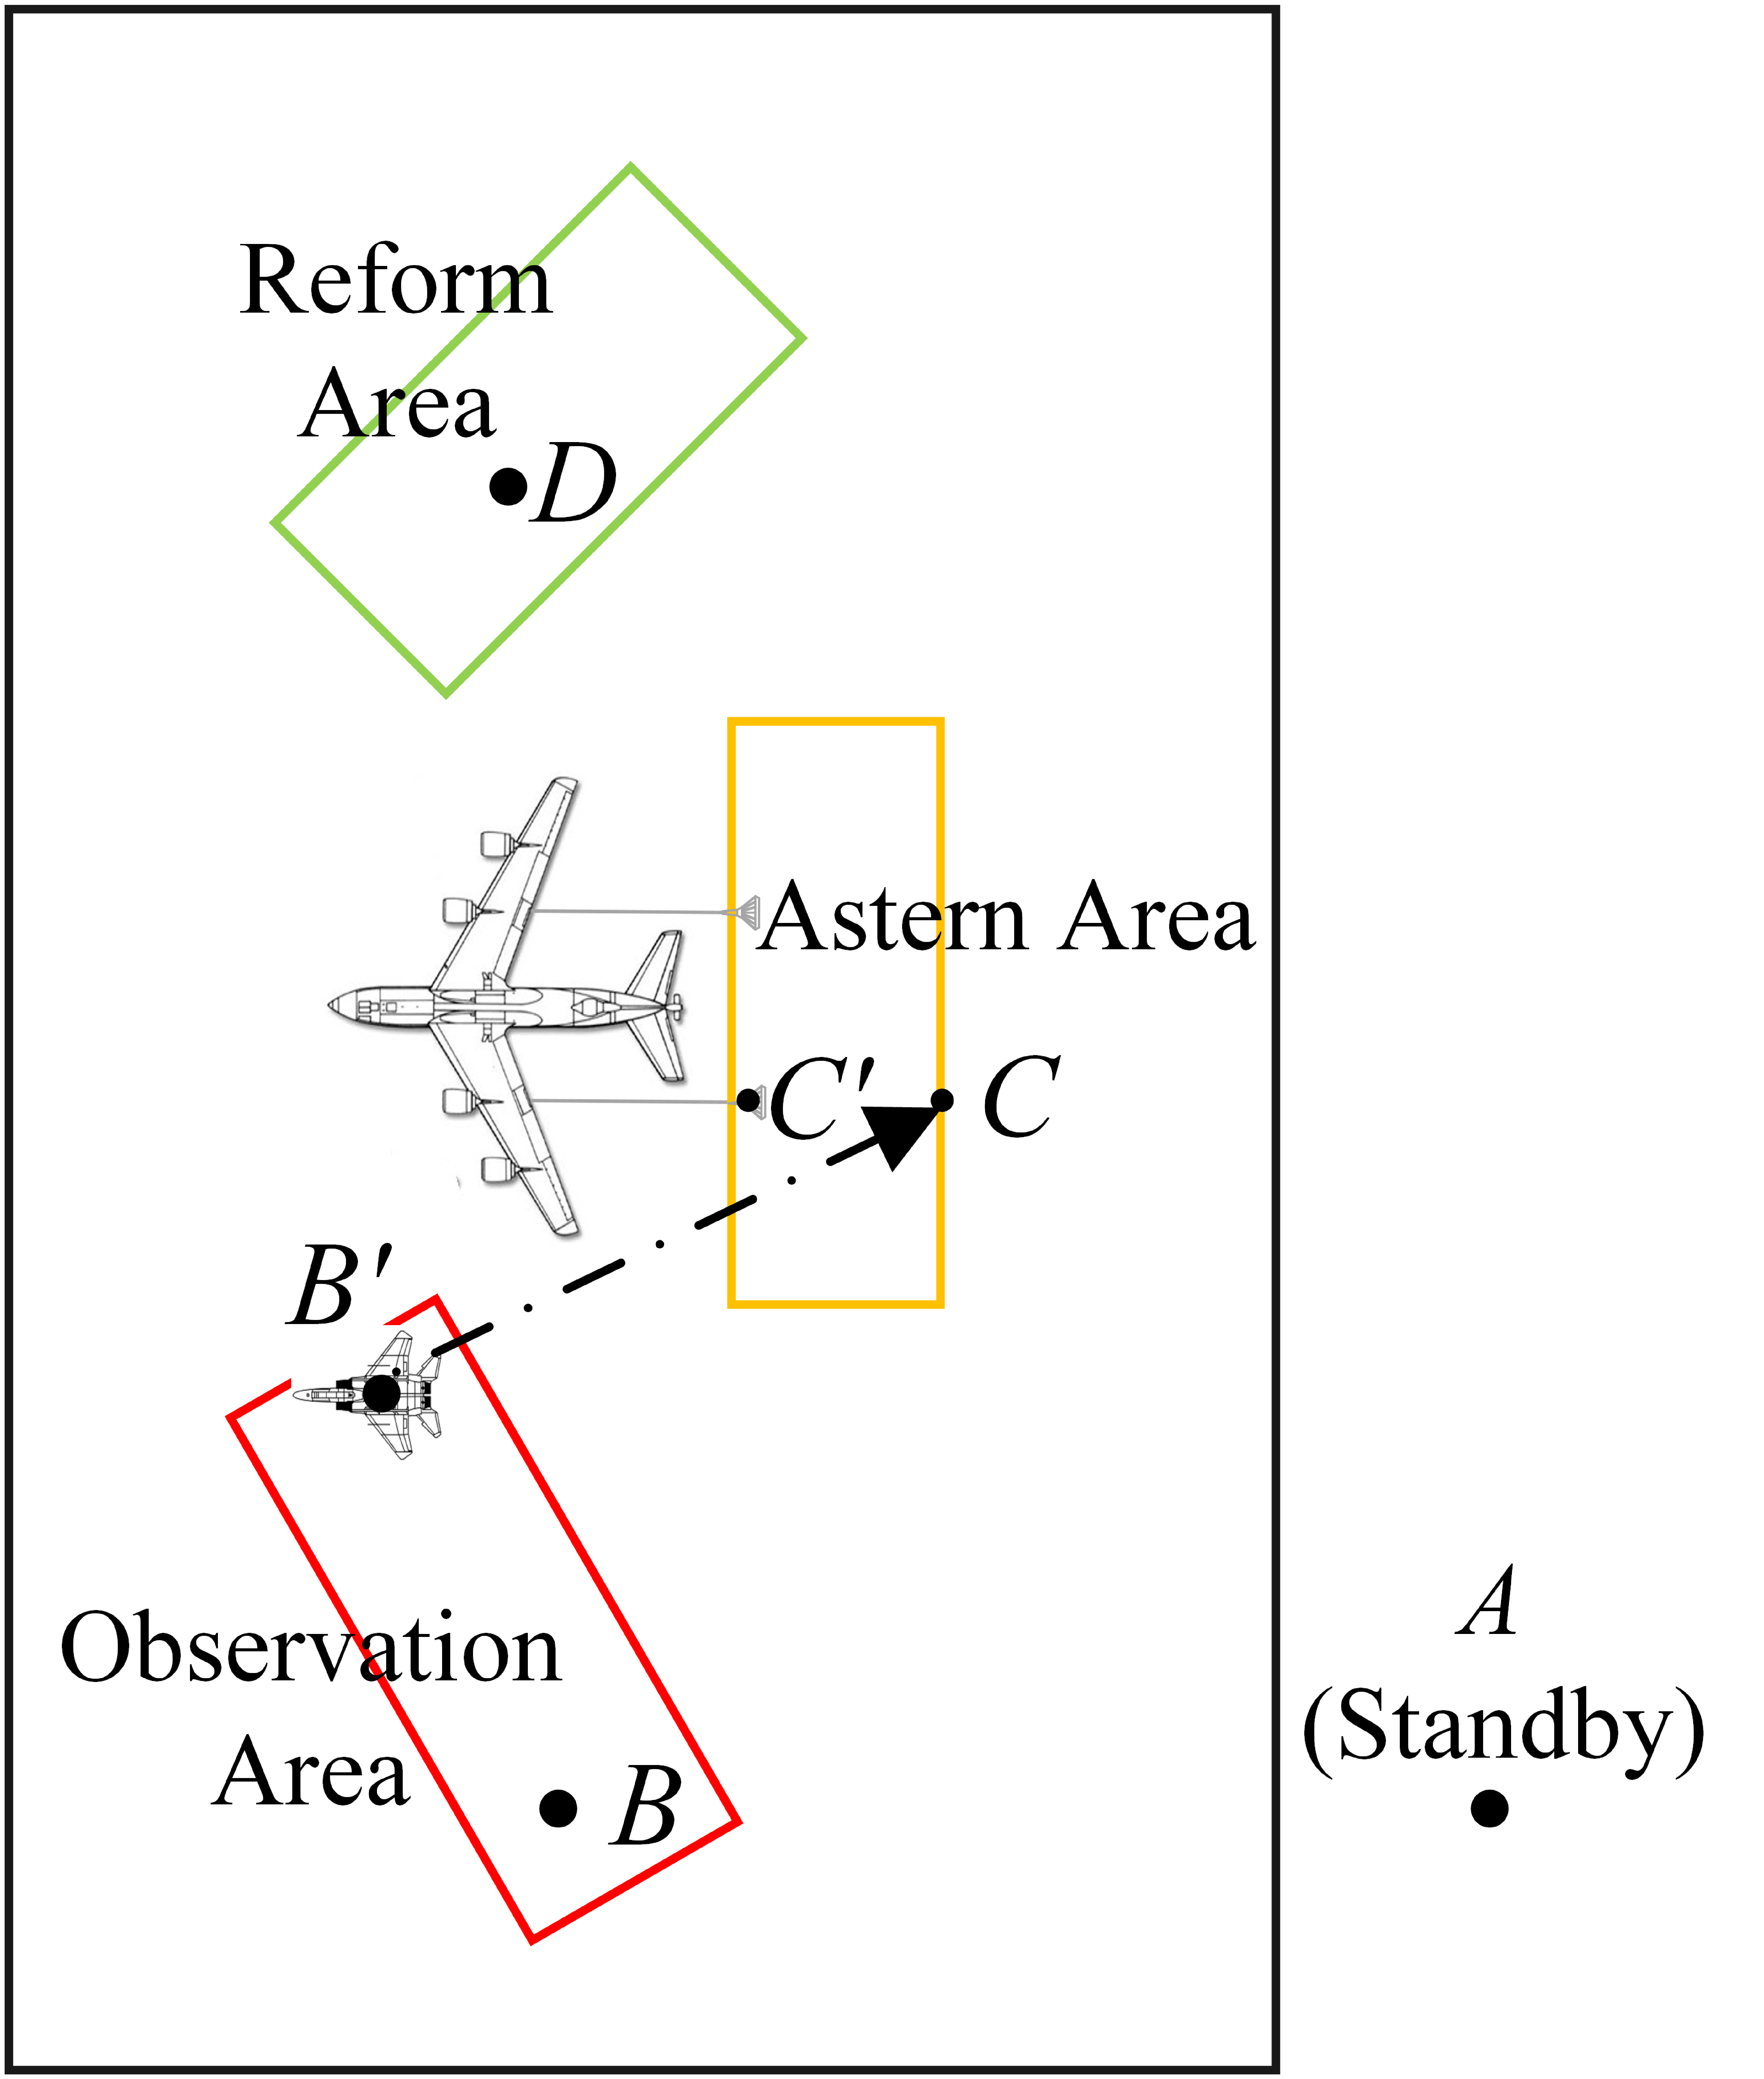
\includegraphics[scale=0.035]{Figures/Figs_Ch14/Fig7a_Refueling_Init}}\qquad
	\subfloat[REFUELING-CAPTURE MODE]{\label{fig:refuelingcap}
		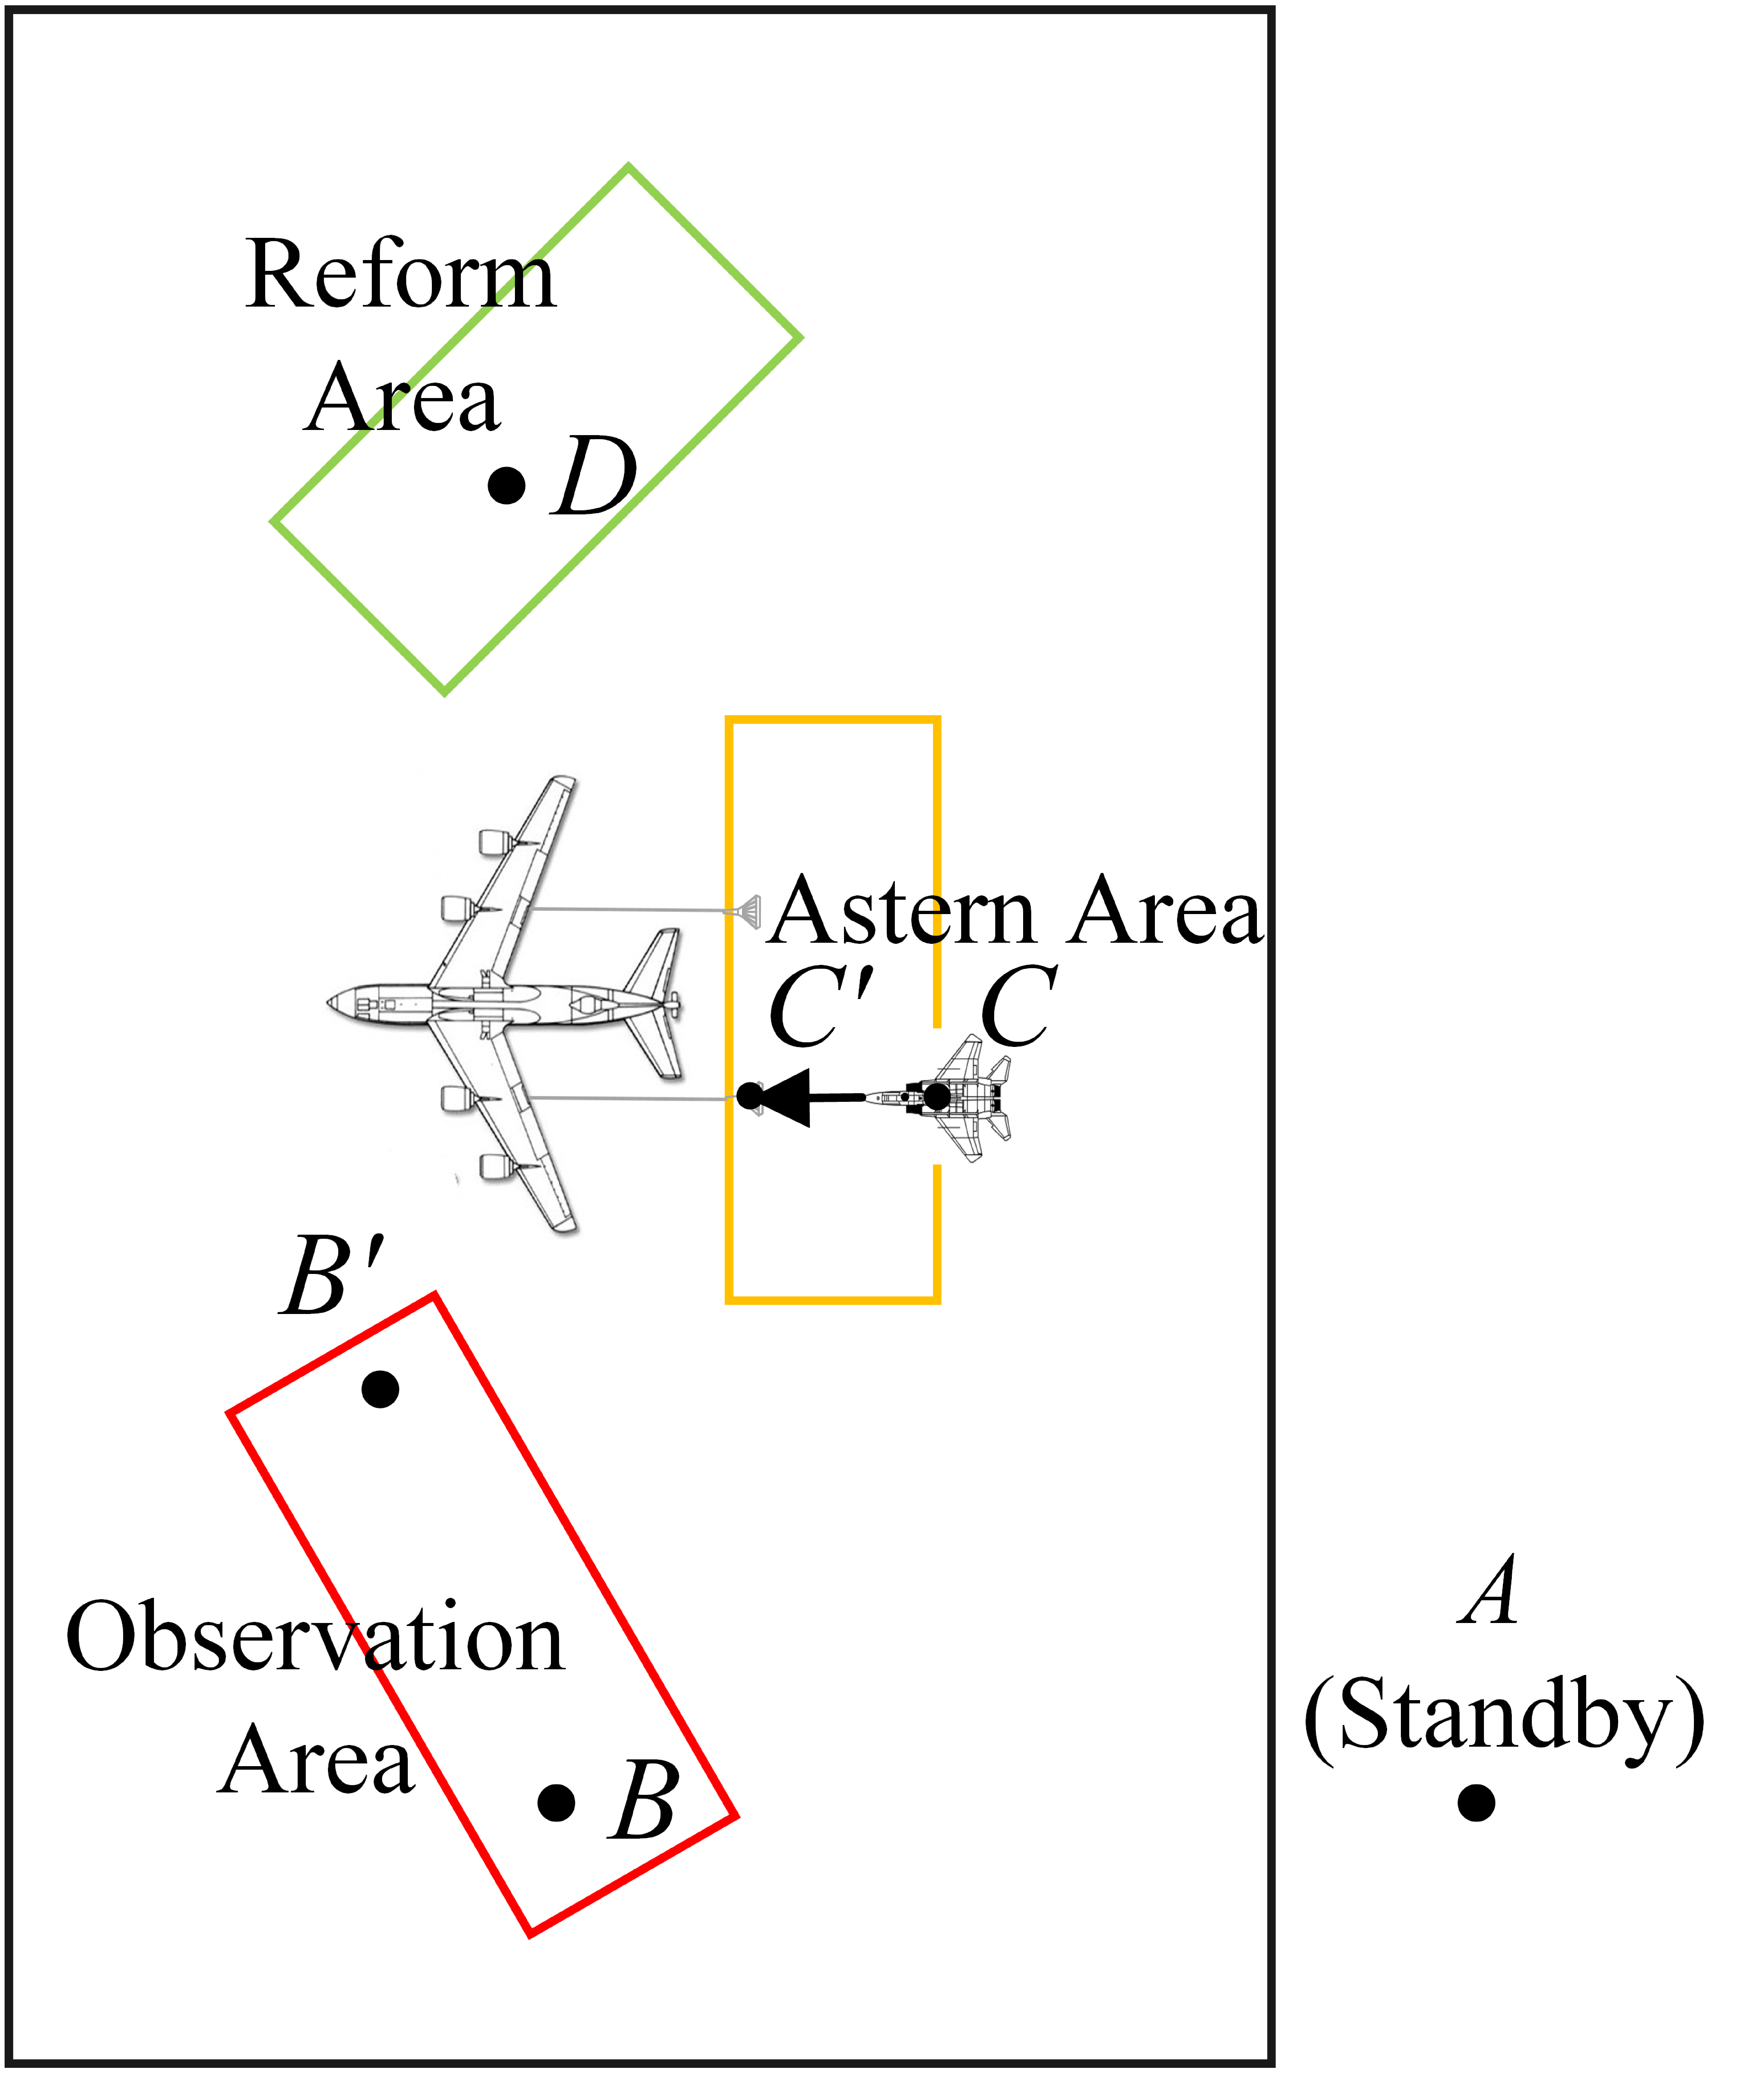
\includegraphics[scale=0.035]{Figures/Figs_Ch14/Fig7b_Refueling_Capture}}\qquad
	\subfloat[JOINING-TRANSFER MODE]{\label{fig:refuelingtran}
		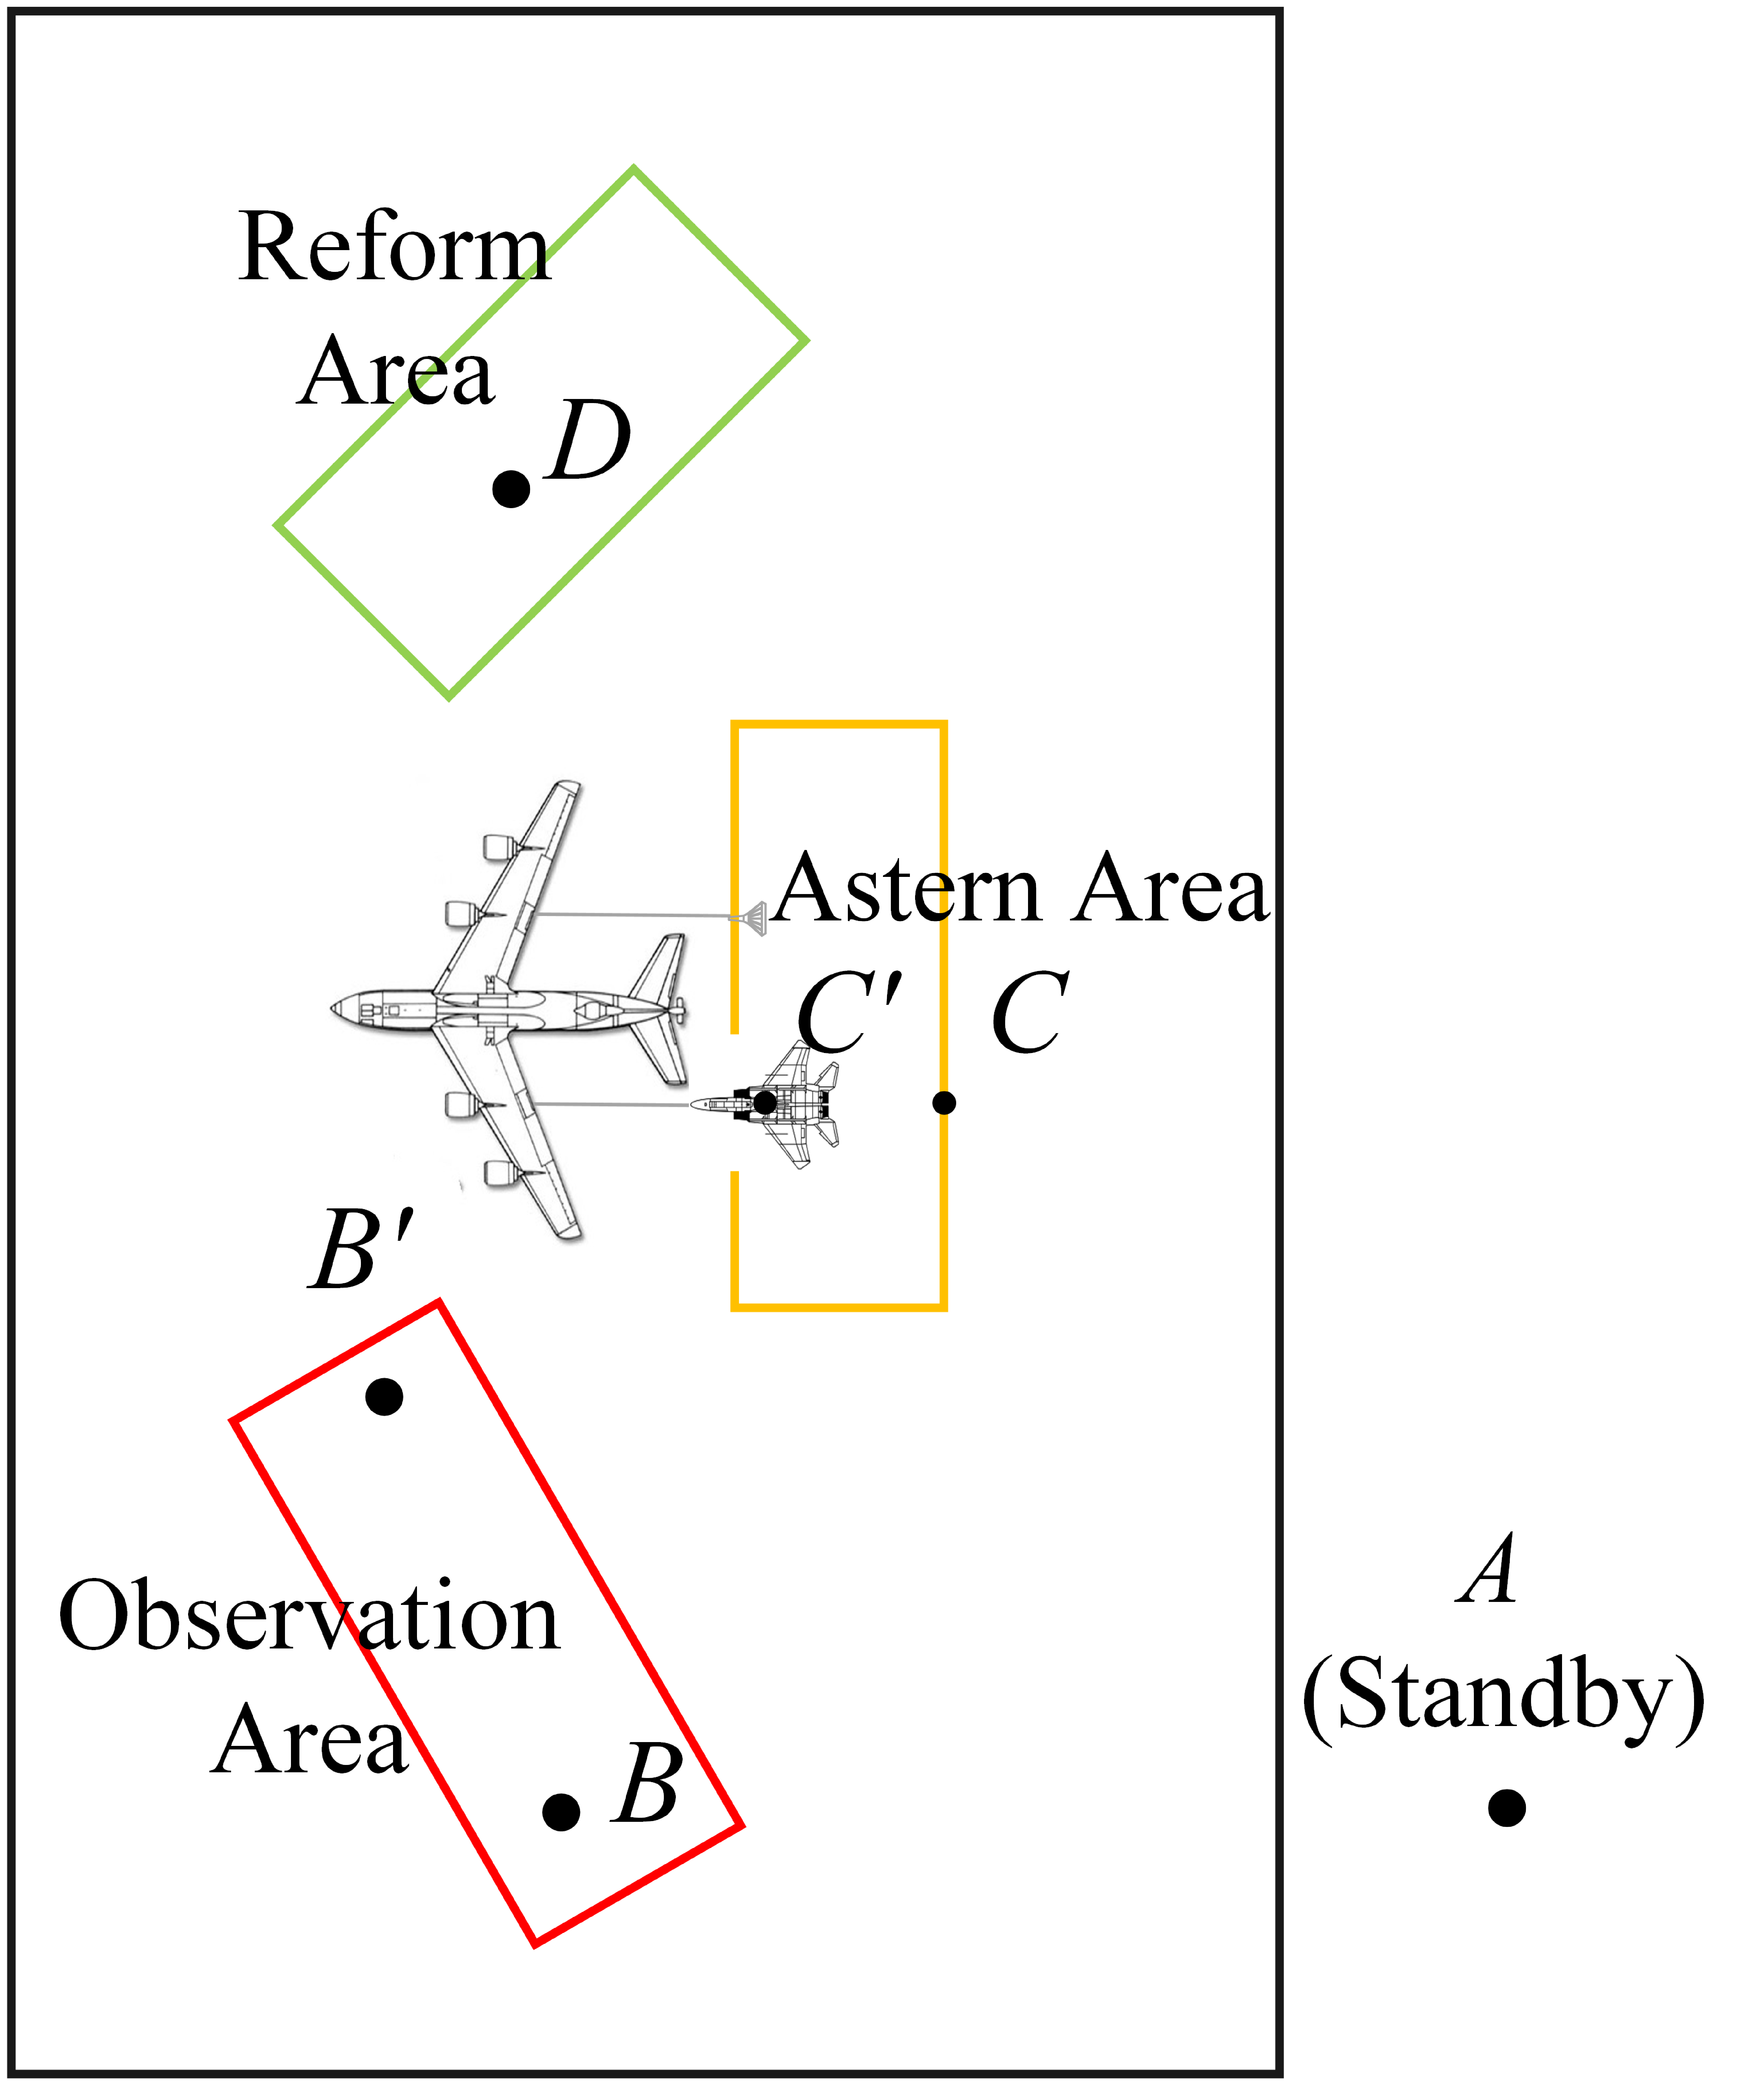
\includegraphics[scale=0.035]{Figures/Figs_Ch14/Fig7c_Refueling_Transfer}}
	\caption{Refueling sub-phase.}
	\label{Fig:refueling}
\end{figure}


\begin{figure}[h]
	\centering
	\subfloat[REFORMING-INIT MODE]{\label{fig:reforminit}
		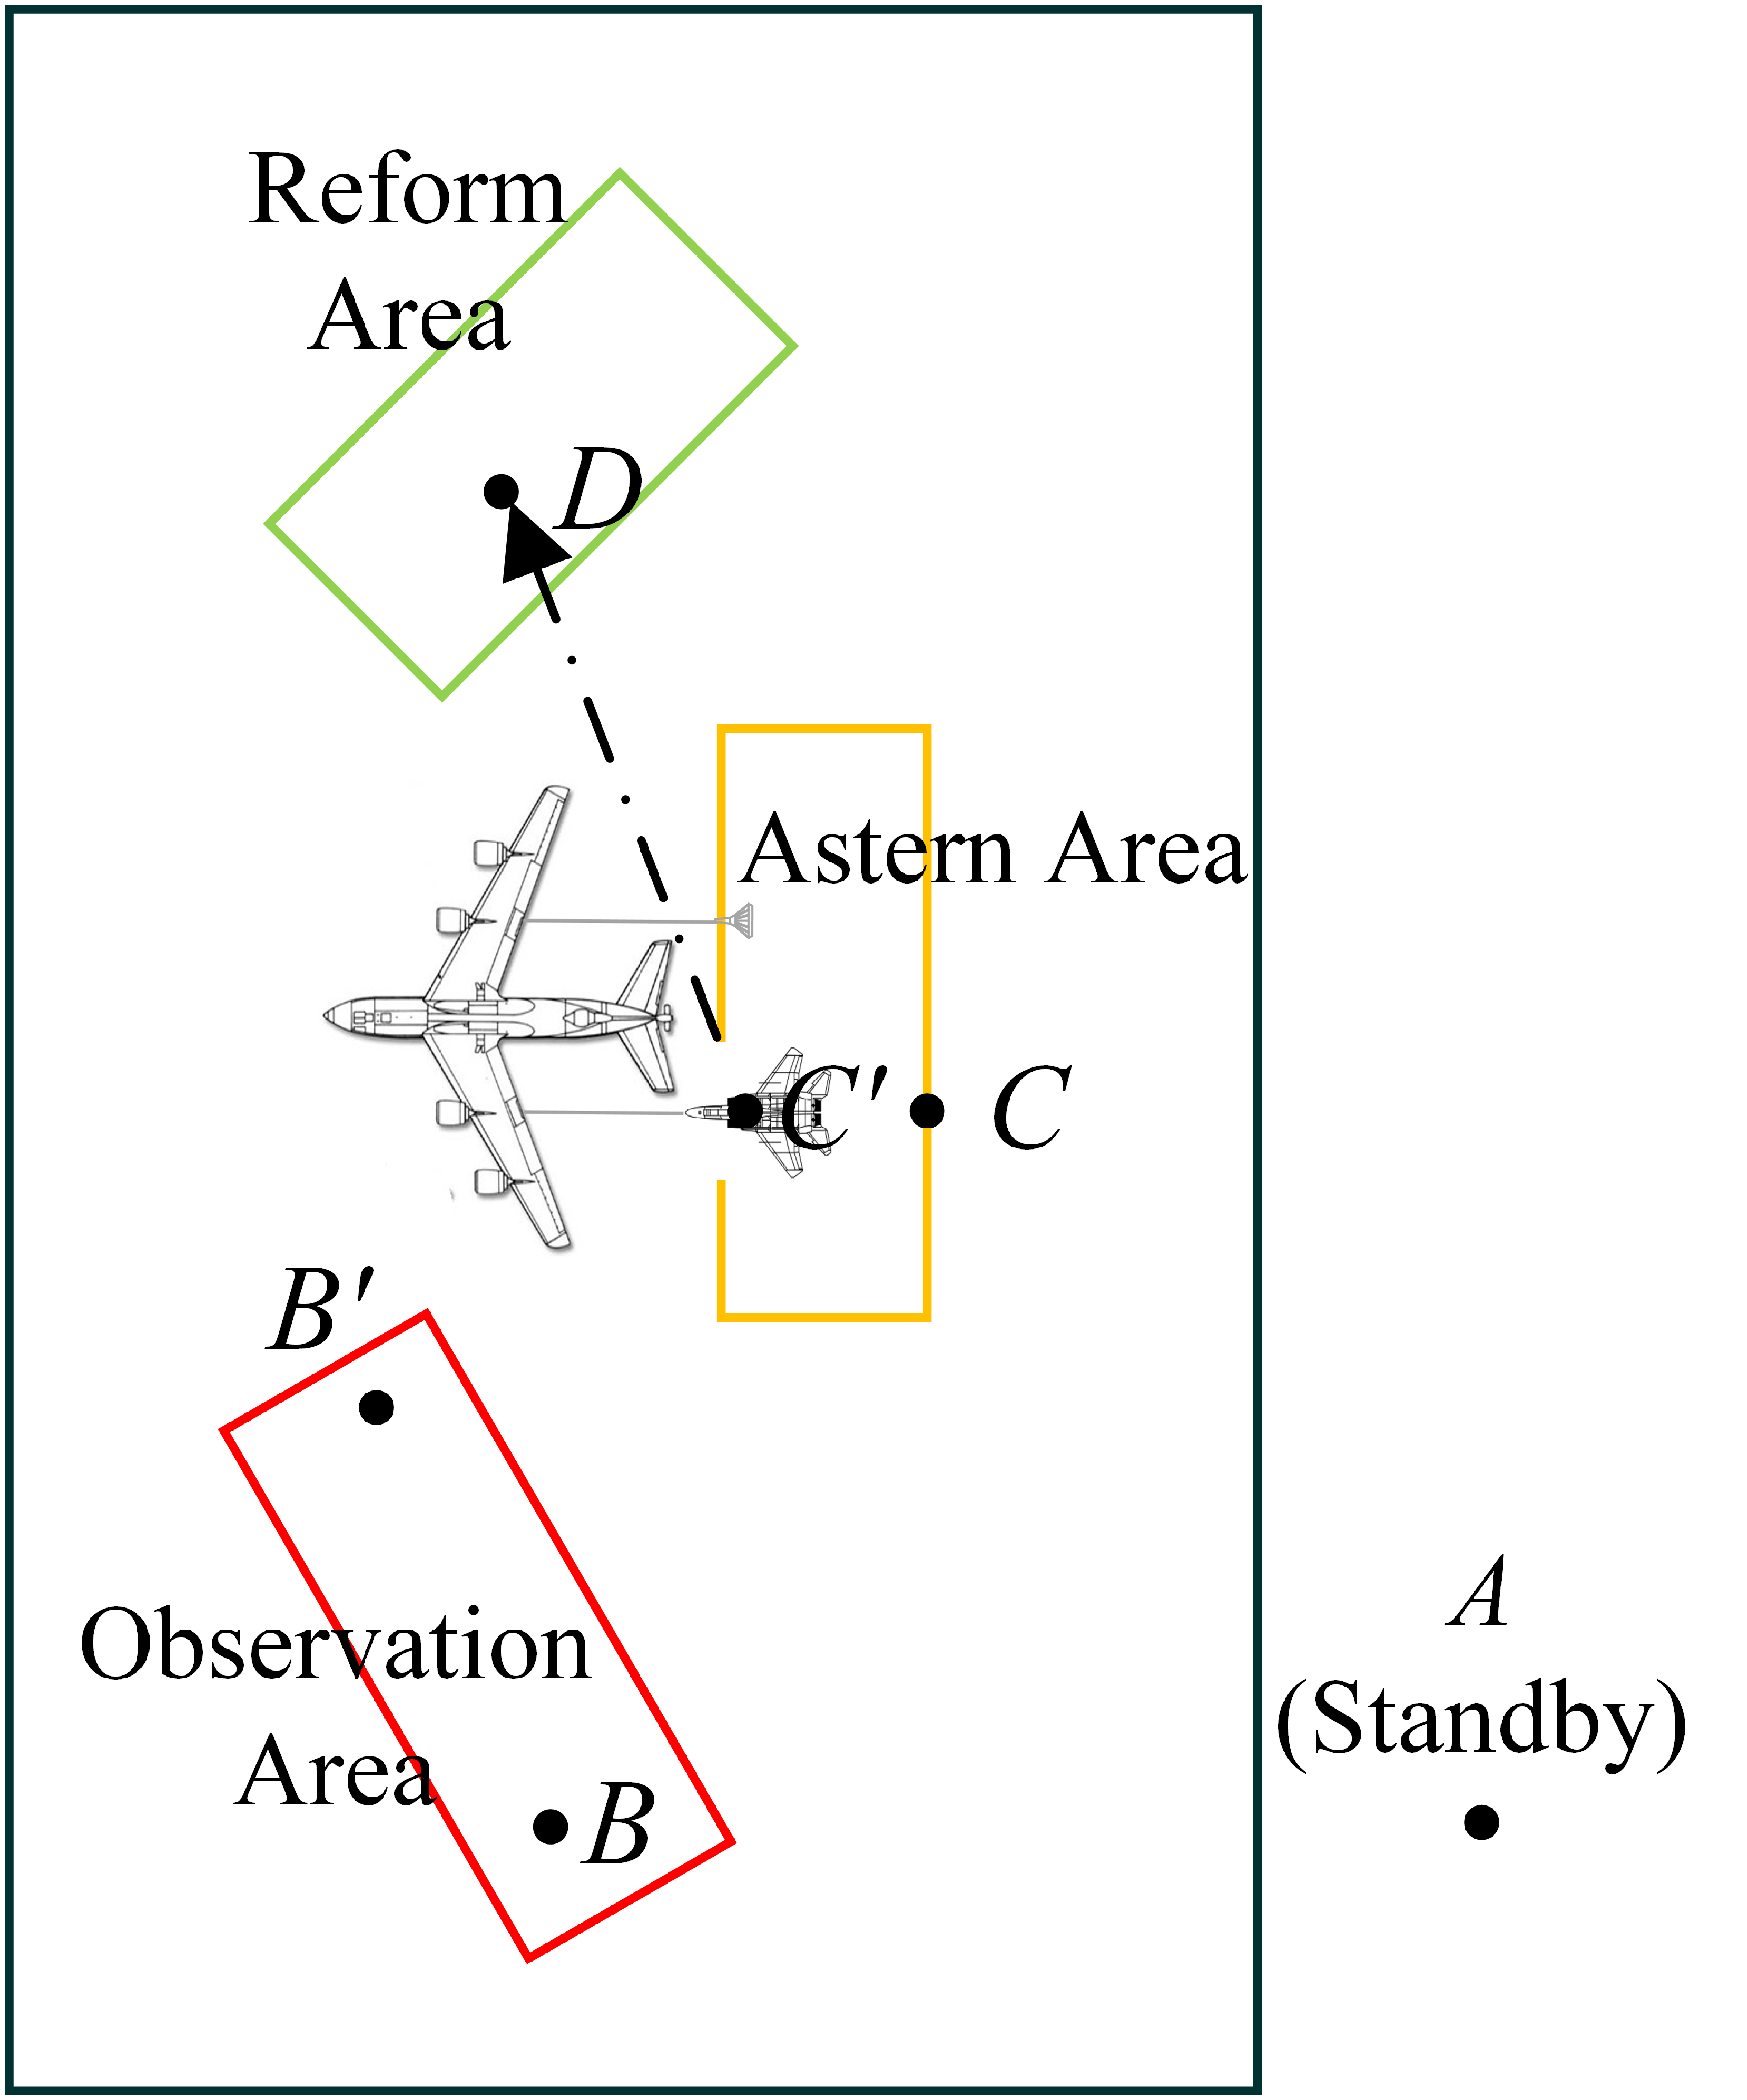
\includegraphics[scale=0.035]{Figures/Figs_Ch14/Fig8a_Reforming_Init}}\qquad
	\subfloat[REFORMING-FORMATION MODE]{\label{fig:reformform}
		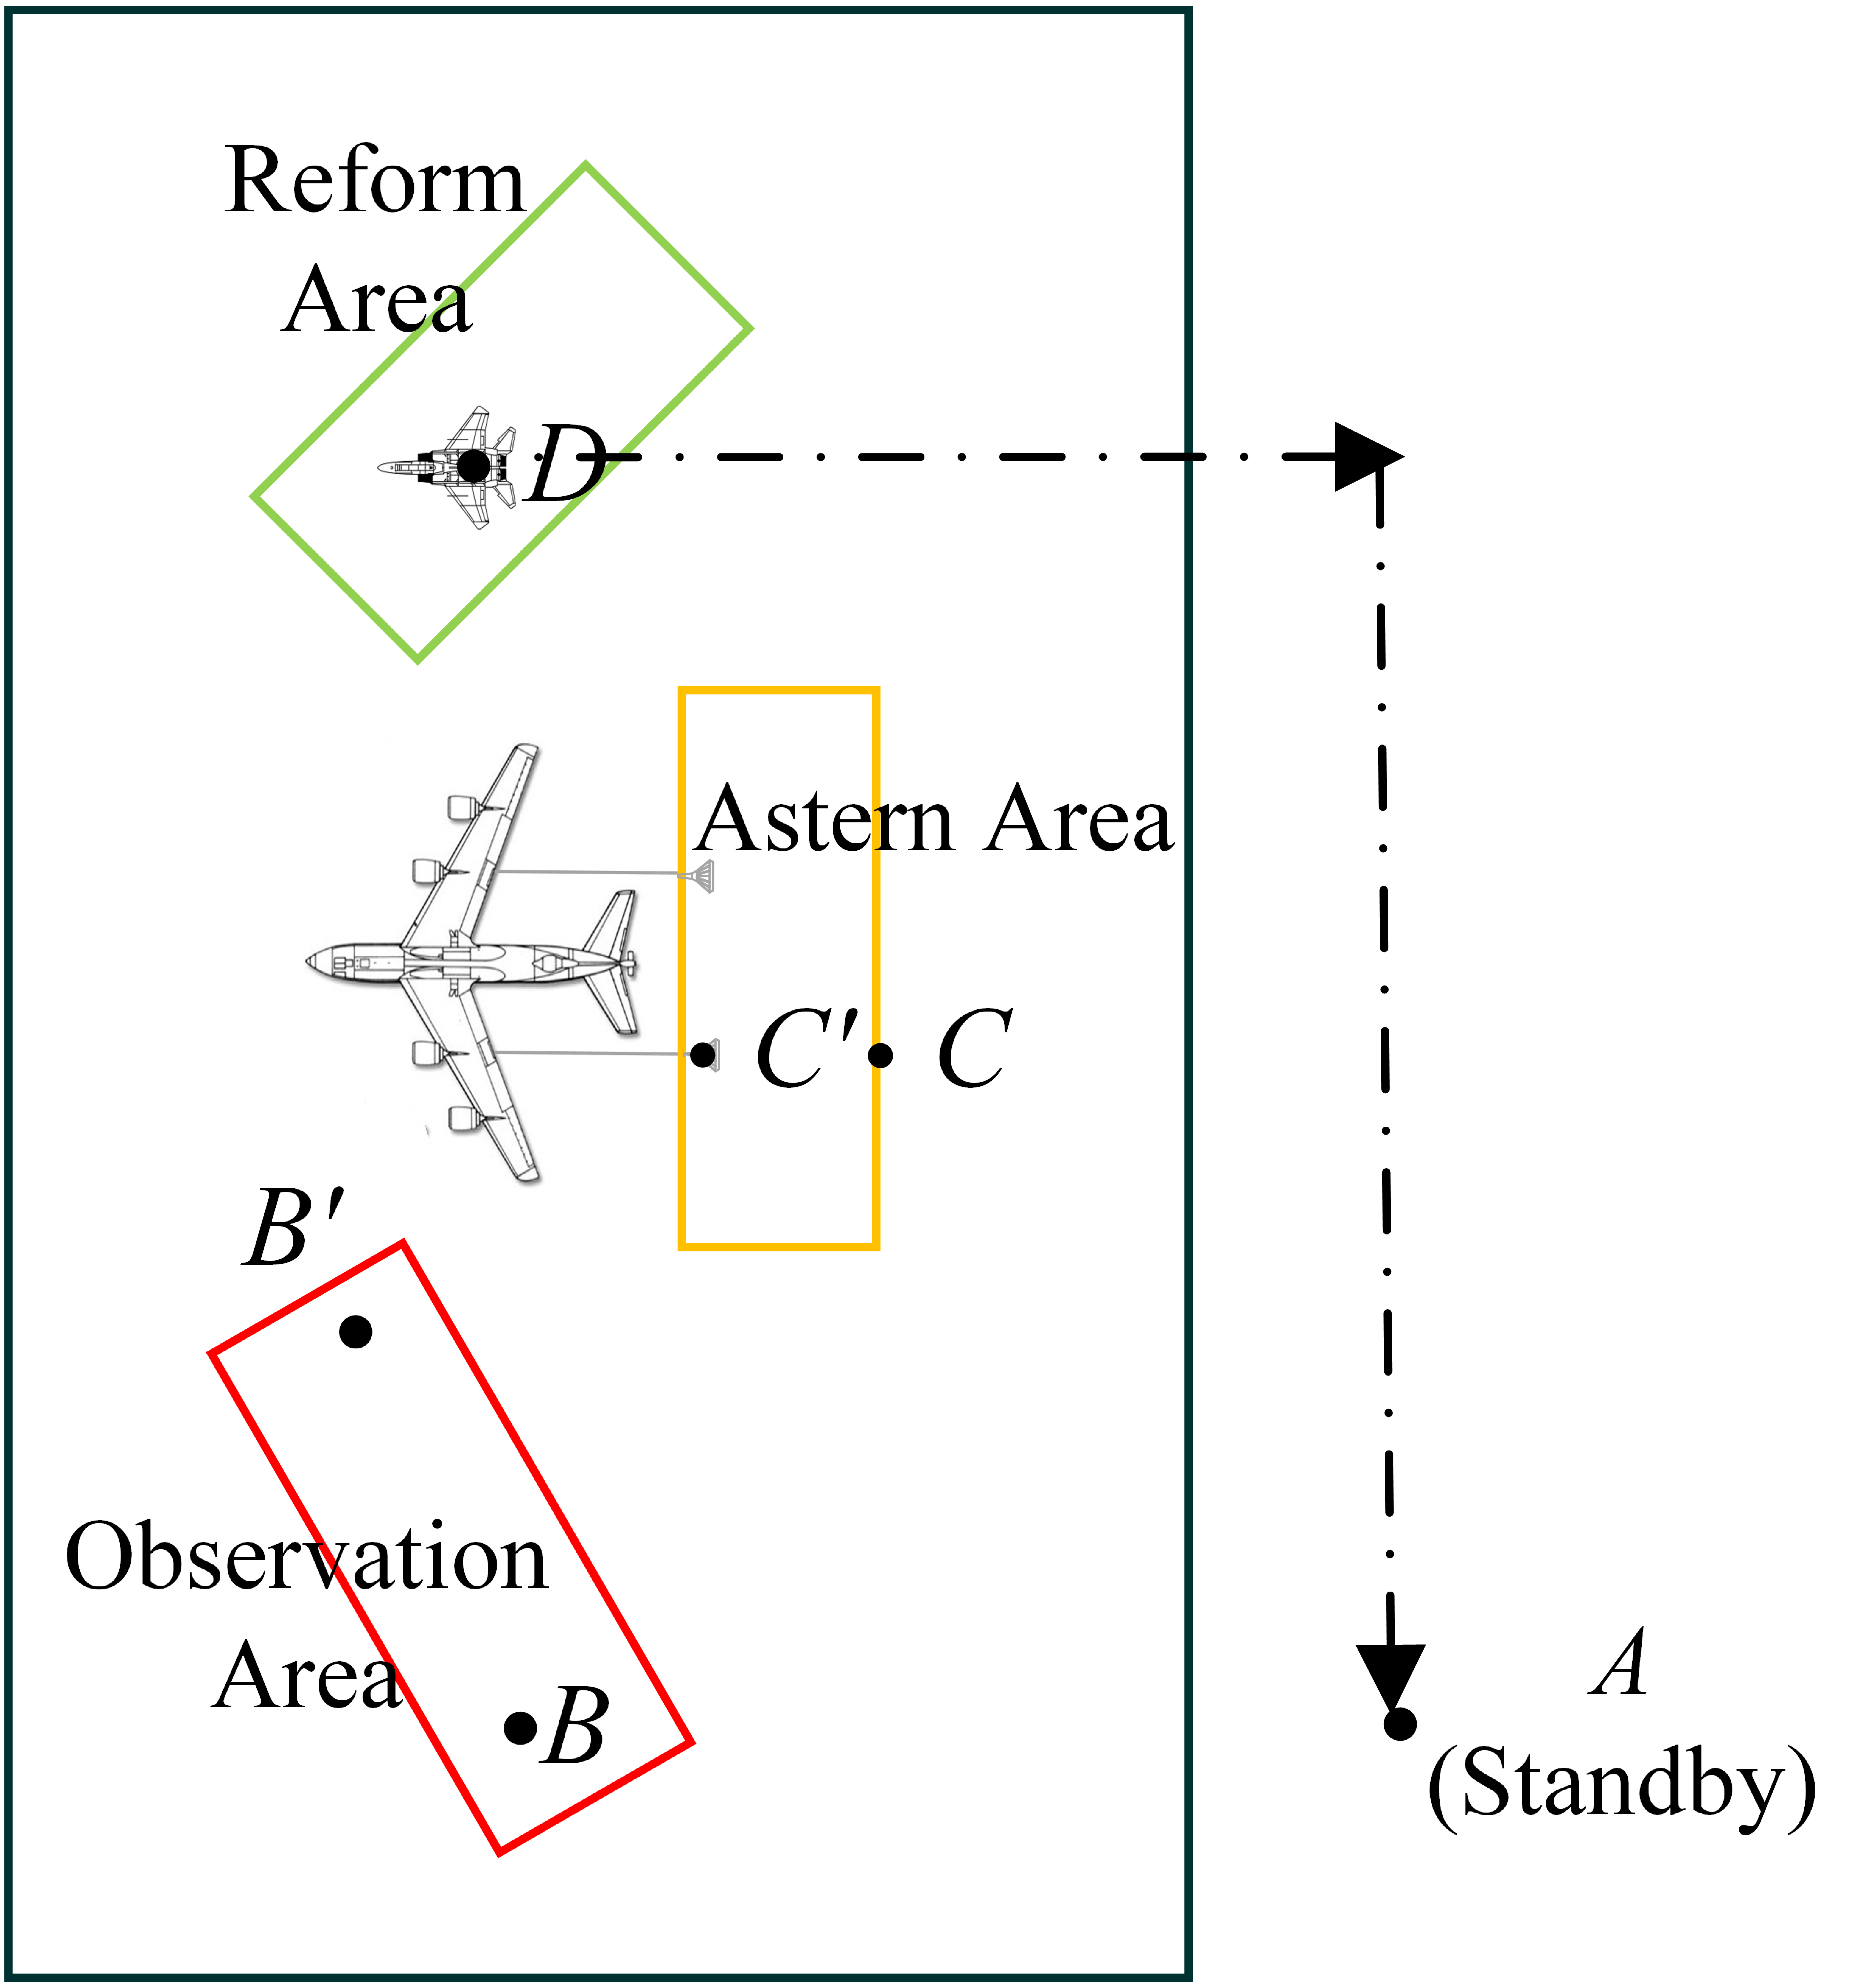
\includegraphics[scale=0.035]{Figures/Figs_Ch14/Fig8b_Reforming_Form}}
	\caption{Reforming sub-phase.}
	\label{Fig:reforming}
\end{figure}



\hspace{-1.5em}\textbf{c) Reforming Sub-Phase:} Reforming refers to the sub-phase where the receiver disconnects with the tanker, flies to the reform area and then leaves the formation. It has two modes.
\begin{enumerate}
	\item \textbf{REFORMING-INIT MODE}: The receiver is cleared for disconnection and then flies to the reform area. As shown in Fig. \ref{Fig:reforming}\subref{fig:reforminit}, the control objective is to control the receiver flying to point $ D $ and then keep the position.
	\item \textbf{REFORMING-FORMATION MODE}: The receiver rejoins the flight formation and then leaves the task space, which can be regarded as returning to the withdrawal space to form a circle in the model. As shown in Fig. \ref{Fig:reforming}\subref{fig:reformform}, the control objective is to control the receiver to maneuver from point $D$ to the withdrawal space.
\end{enumerate}


%\end{verbatim}



\subsection{Safety Issues}
\label{sec:safetyissue}
This subsection summarizes the common failure behaviors in aerial refueling. They are the health information that should be taken into consideration when making decisions. These failures mainly happen in those subsystems shown in Table \ref{tab:subsystem}.

\begin{table*}[!htb]
	\centering
	\begin{threeparttable}
		\caption{Subsystem Information}
		\label{tab:subsystem}
		\begin{tabular}{|l|l|p{11cm}|}
			\hline
			Category & Name & Basic Requirement \\ \hline
			\multirow{4}*{Receiver} & Navigation &  Provide data about the relative position and velocity between receivers and tankers to facilitate docking \\ \cline{2-3}
			~ & Control & Keep the receiver's position and velocity within an allowable range according to its current mode, to avoid collision with other aircraft and achieve successful docking \\ \cline{2-3}
			~ & Fuel & Provide the necessary fuel for flight \\ \cline{2-3}
			~ & Engine & Provide the necessary power and thrust for flight \\ \hline
			\multirow{2}*{Connection} & Drogue\&probe & Establish robust contact between the drogue and probe, and then transfer fuel from the tanker to the receiver \\ \cline{2-3}
			~ & Datalink & Exchange data for communication and high-accuracy computation of relative locations \\ \hline
			Tanker& Tankersafety\tnote{1} &  Facilitate the stable connection and transfer the fuel \\ \hline
		\end{tabular}
		\begin{tablenotes}\footnotesize
			\item[1] To avoid redundancy, the tanker is modeled as a whole instead of with different subsystems like those of the receiver
		\end{tablenotes}
	\end{threeparttable}
	
\end{table*}

Most of their failure behaviors can be depicted as the holon shown in Fig. \ref{fig:failure-automaton}. According to concrete requirements, a subsystem can have more states to describe the health, but only three different health states of each subsystem are considered here, namely \textit{normal}, \textit{minor damage} and \textit{critical damage}. ``Normal'' state represents that the system satisfies the basic requirements with all components being healthy. ``Minor damage'' state represents that although there are some failures in the system, the system can still satisfy the basic requirements. ``Critical damage'' state represents that the system can no longer satisfy the basic requirements. 

Transitions among different states, namely $ x $\_suspension, $ x $\_recover and $x$\_break \allowbreak -down are detected by low-level modules, where $ x $ refers to an exact subsystem name as shown in Table \ref{tab:subsystem}, e.g., Navigation. They can be defined according to the specific designers' purpose. For example, the transitions of the Navigation subsystem are given as follows:

\begin{itemize}
	\item \textbf{Navigation\_suspension}: The precision of navigation data has degraded to  be lower than a specified threshold, but it can still satisfy the basic requirement of the navigation subsystem. Degradation reasons are multiple, such as bad weather for cameras, radars \& lasers, multi-path effects, hostile jamming and spoofing for GPS \cite{THOMAS201414}.
	\item \textbf{Navigation\_recover}: Precision quality exceeds a specified threshold, and the Navigation subsystem is healthy again.
	\item \textbf{Navigation\_breakdown}: The \textit{minor damage} state has lasted more than a given threshold time or the data provided do not fulfill the basic requirement of the navigation subsystem.
\end{itemize}

Owing to the special characteristics of the Fuel subsystem, there is no $ x $\_recover transition in this subsystem. Its holon can be seen in Fig. \ref{fig:fuelfailureautomation}.
\begin{figure}[h]
	\begin{center}
		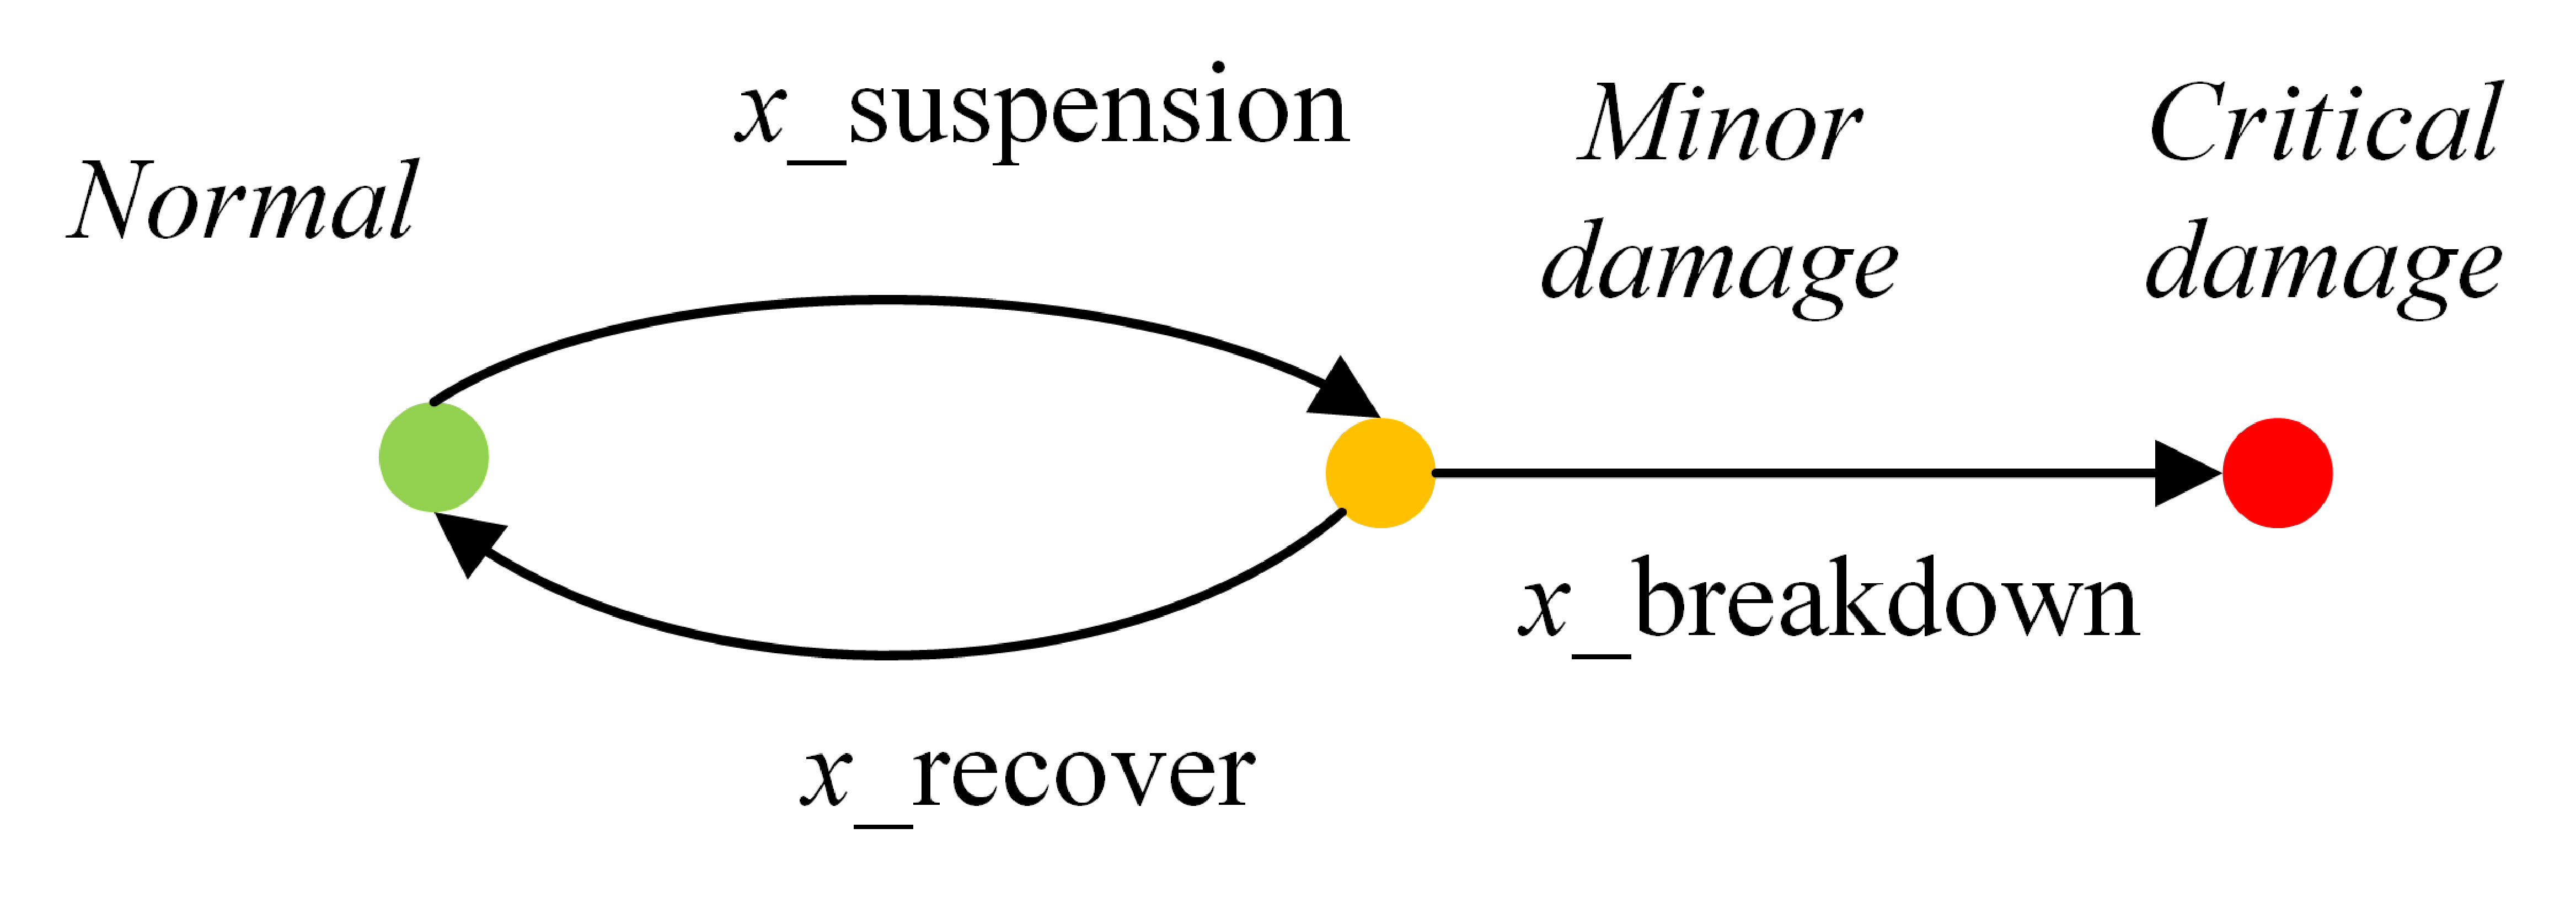
\includegraphics[width=0.5\textwidth]{Figures/Figs_Ch14/Fig9a_GeneralHolon}
		\par\end{center}
	\caption{The general holon of subsystems.}
	\label{fig:failure-automaton} 
\end{figure}

\begin{figure}[h]
	\begin{center}
		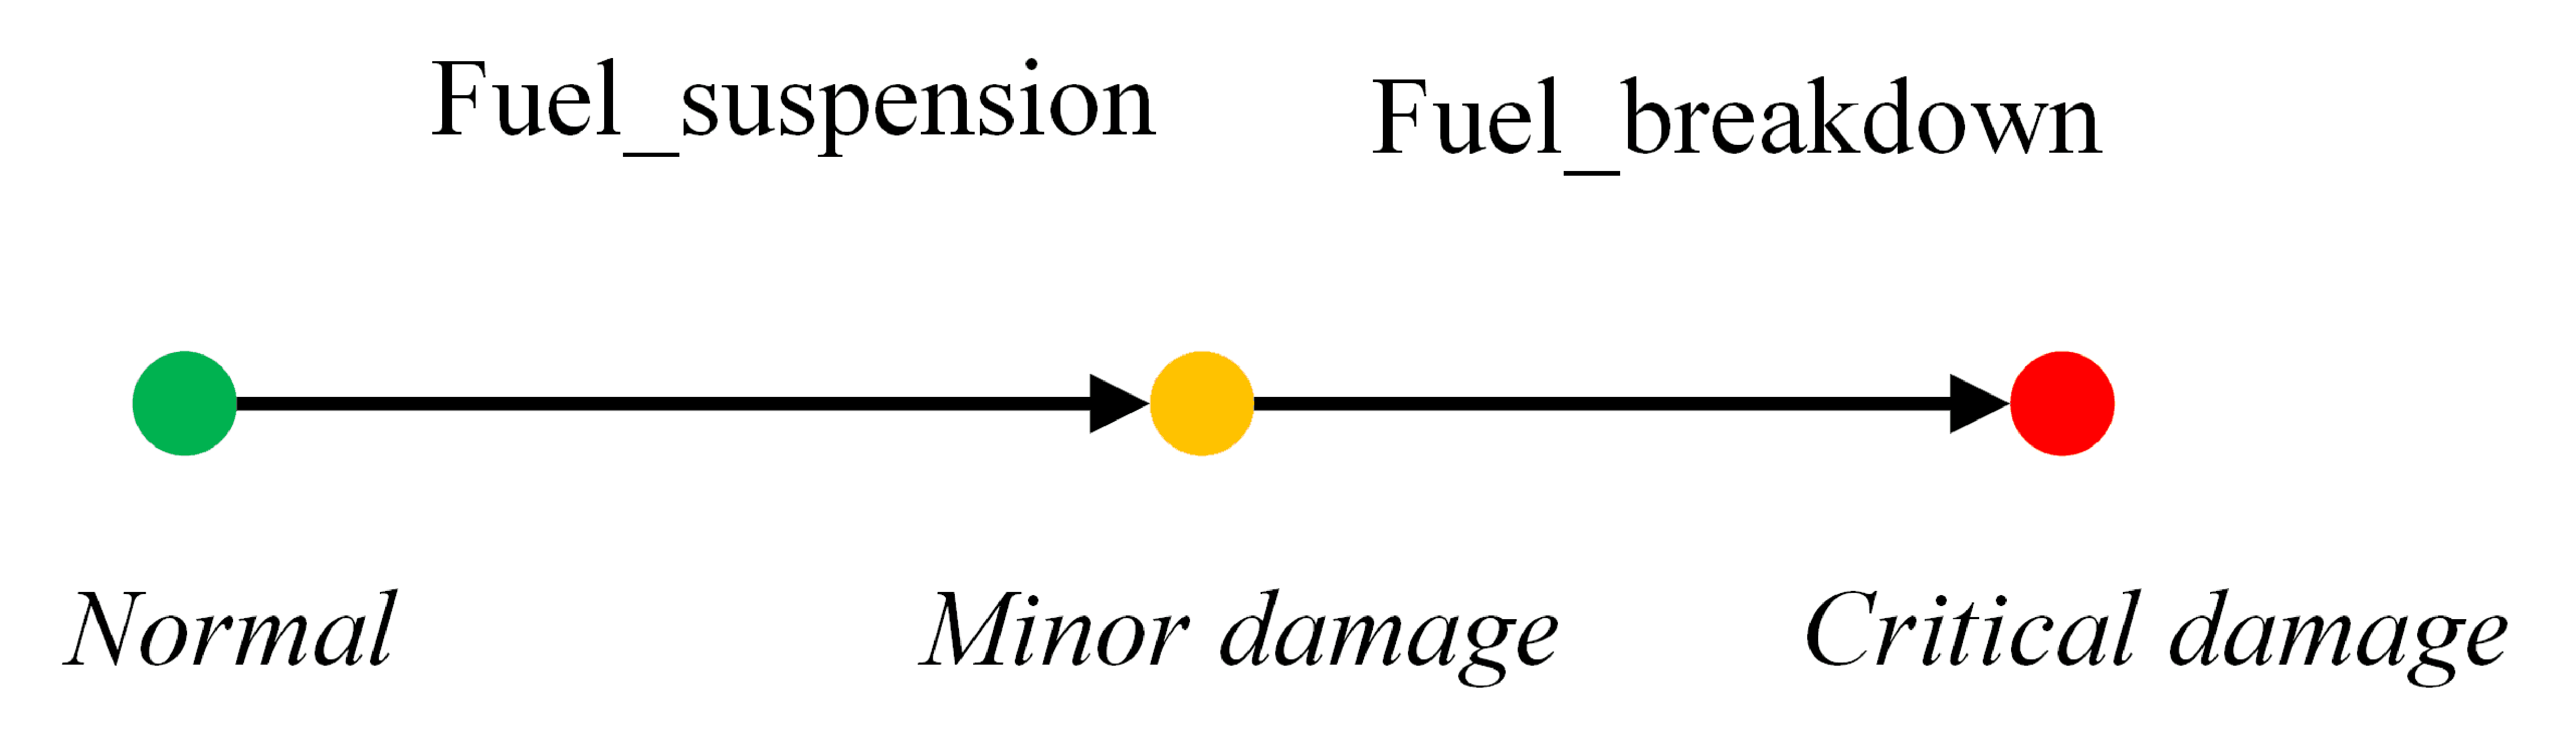
\includegraphics[width=0.5\textwidth]{Figures/Figs_Ch14/Fig9b_FuelHolon}
		\par\end{center}
	\caption{The holon of Fuel subsystem. To be consistent with other subsystems, the exhaustion of fuel is called \textit{Fuel\_breakdown} here.}
	\label{fig:fuelfailureautomation} 
\end{figure}	

\section{User Requirements and Event Definitions}
\label{sec:req}
This section textually describes the requirements of aerial refueling. Functional demands and safety requirements are summarized from common user requirements of the logic control system; they will guide the design of plants and specifications, respectively. Event definitions are also provided here.

\subsection{User Requirements}
In engineering practice, aerial refueling systems have to satisfy multiple functional demands and safety requirements, as summarized in Table \ref{tab:functiondemand} and Table \ref{tab:safetyreq}. Functional demands deal with what functions should exist in the system, like ``the receiver can be forced by pilots to try connecting with the tanker even when the health conditions do not allow so". They are used to guide the design of plants in STS. Safety requirements deal with what behaviors are illegal, e.g. ``when control subsystem breaks down, the receiver cannot continue the current AAR task". They are used to design the specifications in STS. 
%??????	
%\begin{longtable}{cl}
%	\caption{Functional Demands \label{tab:functiondemand}}  \\
%	\hline\hline 
%	Name & Definition \\ 
%	\hline\hline
%	\endfirsthead
%	\multicolumn{2}{c}{{\tablename\ \thetable{} -- Continued from previous page}} \\
%	\hline\hline
%	Name & Definition \\
%	\hline \hline
%	\endhead
%	\hline \multicolumn{2}{r}{{Continued on next page}} \\
%	\endfoot
%	\hline\hline
%	\endlastfoot
%	SR1	& Entering and staying in STANDBY MODE are allowed when Navigation, Control, Engine, Drogue\&probe, Datalink and Tankersafety subsystems are at \textit{minor damage} or \textit{normal}, and Fuel subsystem is at \textit{normal}. If this requirement is not satisfied, transitions to STANDBY MODE are forbidden and  transitions to RTL should be made. \\ 
%    SR2 & Entering and staying in RTL MODE are allowed when Navigation, Fuel and Engine are at \textit{minor damage} or \textit{normal}. If not, transitions to RTL MODE are forbidden and transitions to EL MODE should be made. \\  
%    SR3	& The transition from STANDBY MODE to \allowbreak JOINING-INIT MODE is allowed when all the subsystems are at \textit{normal}. If not, transitions to JOINING-INIT MODE are forbidden and the receiver should wait in STANDBY MODE. \\ 
%    SR4 & Staying at JOINING-WAIT MODE is allowed when Fuel subsystem is at \textit{normal} and other subsystems are at \textit{minor damage} or \textit{normal}. If not, transitions to JOINING-WAIT MODE are forbidden and transitions to the withdrawal phase should be made. \\ 
%    SR5 & If the waiting time at JOINING-WAIT exceeds a specified threshold, then the receiver should make a transition to STANDBY MODE. \\ 
%    SR6	& Entering REFUELING-INIT MODE is allowed when Navigation, Engine, Datalink and Tankersafety subsystems are at \textit{minor damage} or \textit{normal}, while Control, Fuel and Drogue\&probe subsystems are at \textit{normal}. If not, the receiver, even cleared for connection, should keep waiting at JOINING-WAIT MODE or make transitions to the withdrawal phase. \\ 
%    SR7 & Staying at REFUELING-CAPTURE MODE or REFUELING-TRANSFER MODE (when the fuel transfer is not finished) is allowed when all the subsystems are at \textit{normal}. If this requirement is not satisfied, the receiver is not allowed to stay at this mode. Under this situation, if Navigation, Engine, Datalink and Tankersafety subsystems are at \textit{minor damage} or \textit{normal}, while Control, Fuel and Drogue\&probe subsystems are at \textit{normal}, the receiver should retreat to REFUELING-INIT MODE. Otherwise, the receiver should make transitions to the withdrawal phase. (to be continued in Table \ref{tab:safetyreq2}) \\ 
%    SR8 & When the fuel transfer is finished, staying at REFUELING-TRANSFER MODE is allowed when Navigation, Fuel, Engine, Datalink and Tankersafety are at \textit{minor damage} or \textit{normal}, while Control and Drogue\&probe  are at \textit{normal}. If not, the receiver should make transitions to the withdrawal phase. \\	
%    SR9 & When the receiver is waiting for disconnection clearance at REFUELING-TRANSFER MODE after a successful fuel transfer, the receiver should disconnect from the drogue and switch to REFUELING-INIT MODE, if the waiting time exceeds a specified threshold. \\
%    SR10 & Entering and Staying at REFORMING-INIT MODE or REFORMING-FORMATION MODE are allowed when Navigation, Control, Fuel and Engine subsystems are at \textit{minor damage} or \textit{normal}. If not, transitions to the withdrawal phase should be made. \\ 
%  \hline \hline  	
%\end{longtable}



















\begin{table}
	\caption{Functional Demands \label{tab:functiondemand}}
	{\begin{tabular}{@{}lp{15cm}@{}}
			\hline \hline
			Name & Definition \\
			\hline \hline
			FD1 & The receiver, which switches from the task phase to the withdrawal phase, should first try entering STANDBY. If not satisfying the safety requirement for STANDBY MODE (see SR1 in Table \ref{tab:safetyreq}), the receiver should try entering RTL. If still not satisfying the safety requirement for RTL MODE (see SR2 in Table \ref{tab:safetyreq}), the receiver should try entering EL.  \\ 
			FD2 & In EL MODE, if health conditions satisfy the safety requirements (SR1 or SR2), the receiver can switch to STANDBY MODE or RTL MODE. Similarly, the receiver can switch to STANDBY from RTL. \\ 
			FD3 & If the receiver cannot carry on AAR tasks further, it should break away and switch to the withdrawal phase as soon as possible. \\ 
			FD4 & The receiver has to wait for the clearance commands from the tanker to connect or disconnect with the tanker. \\ 
			FD5 & Pilots can manually switch the receiver to the STANDBY, RTL  or EL MODE from any state. When health conditions allow, such instructions should be executed as soon as possible and override any other automatic mode progression. \\ 
			FD6 & Pilots can force the enablement of the connection initiation and fuel transfer initiation (see MCE08 and MCE10 in Table \ref{tab:MCE}), even though such maneuvers are forbidden by the autopilot due to severe health conditions. \\ 
			FD7 & Considering pilots may not know the real-time health information of receivers in timely fashion, when pilots ask the receiver to return to STANDBY MODE, the receiver can go to STANDBY, RTL and EL MODE. When asked to return to RTL MODE, the receiver can go to RTL and EL MODE. When asked to go to EL MODE, it can only switch to EL MODE. \\
			\hline \hline
	\end{tabular}}
\end{table}

~\\[5cm]

\begin{table}
	\caption{Safety requirements in withdrawal phase \label{tab:safetyreq}}
	{\begin{tabular}{@{}lp{15cm}@{}}
			\hline \hline
			Name & Description \\
			\hline \hline 
			SR1	& Entering and staying in STANDBY MODE are allowed when Navigation, Control, Engine, Drogue\&probe, Datalink and Tankersafety subsystems are at \textit{minor damage} or \textit{normal}, and Fuel subsystem is at \textit{normal}. If this requirement is not satisfied, transitions to STANDBY MODE are forbidden and  transitions to RTL should be made. \\ 
			SR2 & Entering and staying in RTL MODE are allowed when Navigation, Fuel and Engine are at \textit{minor damage} or \textit{normal}. If not, transitions to RTL MODE are forbidden and transitions to EL MODE should be made. \\  
			SR3	& The transition from STANDBY MODE to \allowbreak JOINING-INIT MODE is allowed when all the subsystems are at \textit{normal}. If not, transitions to JOINING-INIT MODE are forbidden and the receiver should wait in STANDBY MODE. \\ 
			SR4 & Staying at JOINING-WAIT MODE is allowed when Fuel subsystem is at \textit{normal} and other subsystems are at \textit{minor damage} or \textit{normal}. If not, transitions to JOINING-WAIT MODE are forbidden and transitions to the withdrawal phase should be made. \\ 
			SR5 & If the waiting time at JOINING-WAIT exceeds a specified threshold, then the receiver should make a transition to STANDBY MODE. \\ 
			SR6	& Entering REFUELING-INIT MODE is allowed when Navigation, Engine, Datalink and Tankersafety subsystems are at \textit{minor damage} or \textit{normal}, while Control, Fuel and Drogue\&probe subsystems are at \textit{normal}. If not, the receiver, even cleared for connection, should keep waiting at JOINING-WAIT MODE or make transitions to the withdrawal phase. \\ 
			SR7 & Staying at REFUELING-CAPTURE MODE or REFUELING-TRANSFER MODE (when the fuel transfer is not finished) is allowed when all the subsystems are at \textit{normal}. If this requirement is not satisfied, the receiver is not allowed to stay at this mode. Under this situation, if Navigation, Engine, Datalink and Tankersafety subsystems are at \textit{minor damage} or \textit{normal}, while Control, Fuel and Drogue\&probe subsystems are at \textit{normal}, the receiver should retreat to REFUELING-INIT MODE. Otherwise, the receiver should make transitions to the withdrawal phase. (to be continued in Table \ref{tab:safetyreq2}) \\ 
			SR8 & When the fuel transfer is finished, staying at REFUELING-TRANSFER MODE is allowed when Navigation, Fuel, Engine, Datalink and Tankersafety are at \textit{minor damage} or \textit{normal}, while Control and Drogue\&probe  are at \textit{normal}. If not, the receiver should make transitions to the withdrawal phase. \\	
			SR9 & When the receiver is waiting for disconnection clearance at REFUELING-TRANSFER MODE after a successful fuel transfer, the receiver should disconnect from the drogue and switch to REFUELING-INIT MODE, if the waiting time exceeds a specified threshold. \\
			SR10 & Entering and Staying at REFORMING-INIT MODE or REFORMING-FORMATION MODE are allowed when Navigation, Control, Fuel and Engine subsystems are at \textit{minor damage} or \textit{normal}. If not, transitions to the withdrawal phase should be made. \\ 
			\hline \hline	
	\end{tabular}}
\end{table}


\subsection{Event Definitions}
Based on event characteristics of AAR tasks, four types of events are defined here, namely Mode Control Events (MCEs), Mode Input Events (MIEs), Automatic Triggered Events (ATEs) and Subsystem Failure Events (SFEs). MCEs and MIEs are controllable events, while ATEs and SFEs are uncontrollable events. Their detailed descriptions are given as follows.
\begin{enumerate}
	\item \textbf{MCEs}: Commands generated by the autopilot to proceed  automatically. 
	\item \textbf{MIEs}: Instructions sent from pilots to change the automatic AAR procedures. 
	\item \textbf{ATEs}: Detection results of AAR maneuvers. In most cases, an MCE has two possible ATEs, which mean success and failure. For example, the event MCE04 is to control the receiver to fly from the STANDBY position to the observation area, thus this command has two possible results: ``arrived" (``ATE01: Join-Init-Succ")  and ``not arrived" (``ATE02: Join-Init-Fail'').
	\item \textbf{SFEs}: Failure related behaviors of subsystems. These events correspond to transitions including $x$\_suspension, $x$\_recover and $x$\_breakdown, which are presented in Section \ref{sec:safetyissue}.
\end{enumerate}

The exact definition of every MCE is shown in Table \ref{tab:MCE}. As for the MIEs, ATEs and SFEs, their meanings can be easily interpreted from their full names as shown in Fig. \ref{fig:holonaut}$ \sim$\ref{fig:specpilot}. Readers can refer to Appendix \ref{app:event} for their detailed definition tables.

%	\columnbreak
\begin{table}
	\caption{Mode Control Event Definitions \label{tab:MCE}}
	{\begin{tabular}{@{}lp{15cm}@{}}
			\hline \hline
			Name & Description \\
			\hline \hline 
			MCE01 & Control the receiver to stay in EL MODE \\ 
			MCE02 & Control the receiver to stay in RTL MODE \\ 
			MCE03 & Control the receiver to stay in STANDBY MODE \\ 
			MCE04 & Control the receiver flying from STANDBY position to the observation area. \\ 
			MCE05 & Control the receiver to wait in the observation area while avoiding collision with other aircraft. \\ 
			MCE06 & Control the receiver flying to the astern area.\\ 
			MCE07 & Control the receiver to abandon the current connection initiation or fuel transfer initiation and fly to the astern area. \\ 
			MCE08 & Control the receiver to connect its probe with the tanker's drogue. \\ 
			MCE09 & The forced version of MCE08. It  can only be activated by pilots, and cannot be forbidden by autopilots. \\ 
			MCE10 & Control the receiver to keep relatively stationary to the tanker, and open the valve to receive fuel\\ 
			MCE11 & The forced version of MCE10.   It can only be activated by pilots, and cannot be forbidden  by autopilots. \\ 
			MCE12 & Control the receiver to wait in the astern area while keeping connected with the tanker. \\ 
			MCE13 & Control the receiver flying to the reform area.\\ 
			MCE14 & Control the receiver to rejoin the formation. \\
			\hline \hline
	\end{tabular}}
\end{table}	


\section{State Tree Structure Design}
Based on the preparation in section \ref{sec:mode} and \ref{sec:req}, this section shows the AAR failsafe design in the form of state tree structures, whose overall diagram is illustrated in Fig. \ref{fig:root}. 

\begin{figure}[h]
	\begin{center}
		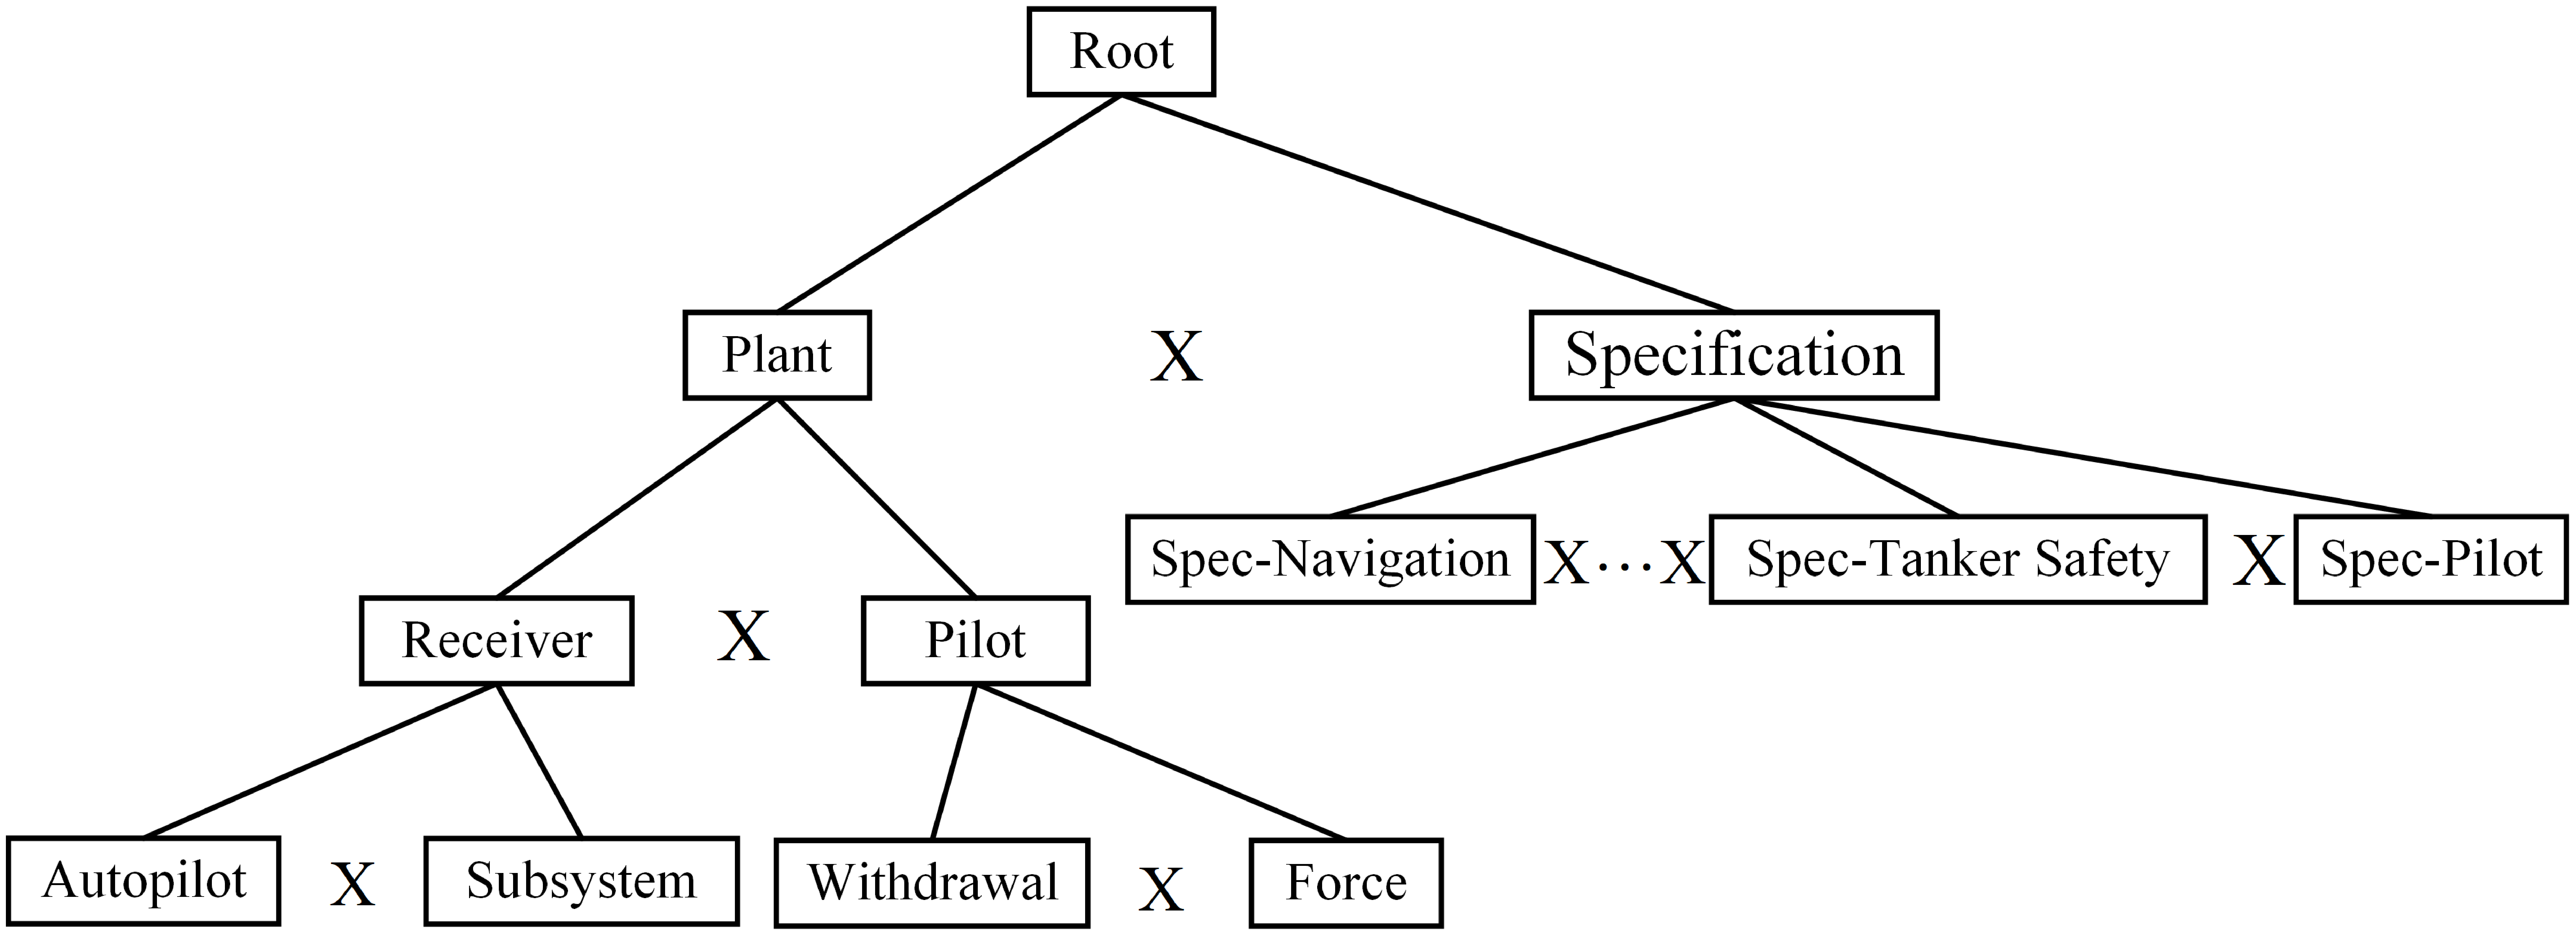
\includegraphics[width=0.8\textwidth]{Figures/Figs_Ch14/Fig10_SAAR}
		\par\end{center}
	\caption{The state tree of AAR with only AND superstates and their components displayed.}
	\label{fig:root} 
\end{figure}

\subsection{Plant design}
In this subsection, the plant design is presented, which includes all the possible behaviors of the aerial refueling tasks. 
\subsubsection{(Receiver) Autopilot}
Autopilot is the AND component of \textit{Receiver}, which is responsible for recording the task procedures of AAR. It is an OR superstate with three simple states (\textit{Standby}, \textit{RTL} and \textit{EL}) and three OR superstates (\textit{Joining}, \textit{Refueling} and \textit{Reforming}), as shown in Fig. \ref{fig:staut}.   

Fig. \ref{fig:holonaut} shows the inner transitions of \textit{Autopilot} (the detailed information of the three superstate is introduced later). In the normal work cycle, the \textit{Autopilot} starts from \textit{Standby} state, goes through the \textit{Joining} superstate  (MCE04), the \textit{Refueling} superstate (MCE06), the \textit{Reforming} superstate (MCE13) and finally returns to the \textit{Standby} state (MCE03). In detail, taking event MCE04 as an example, it leads the receiver from \textit{Standby} state to \textit{Joining} superstate. When this maneuver fails, namely ``ATE01:Join-Init-Fail" happens, the receiver retreats to \textit{Standby} state. Otherwise, ``ATE02:Join-Init-Succ" happens, which leads the \textit{Autopilot} to \textit{Joining} superstate (shown in Fig. \ref{fig:plantjoi}).

When failures happen, the \textit{Autopilot} can retreat to \textit{Standby}, \textit{RTL} and \textit{EL} states from \textit{Joining}, \textit{Refueling} and \textit{Reforming} superstate through events MCE03, MCE02 and MCE01, respectively. Meanwhile, according to the real-time health conditions, the receiver can make transitions among states in the withdrawal phase like from \textit{RTL} to \textit{Standby}.

\begin{figure}[h]
	\begin{center}
		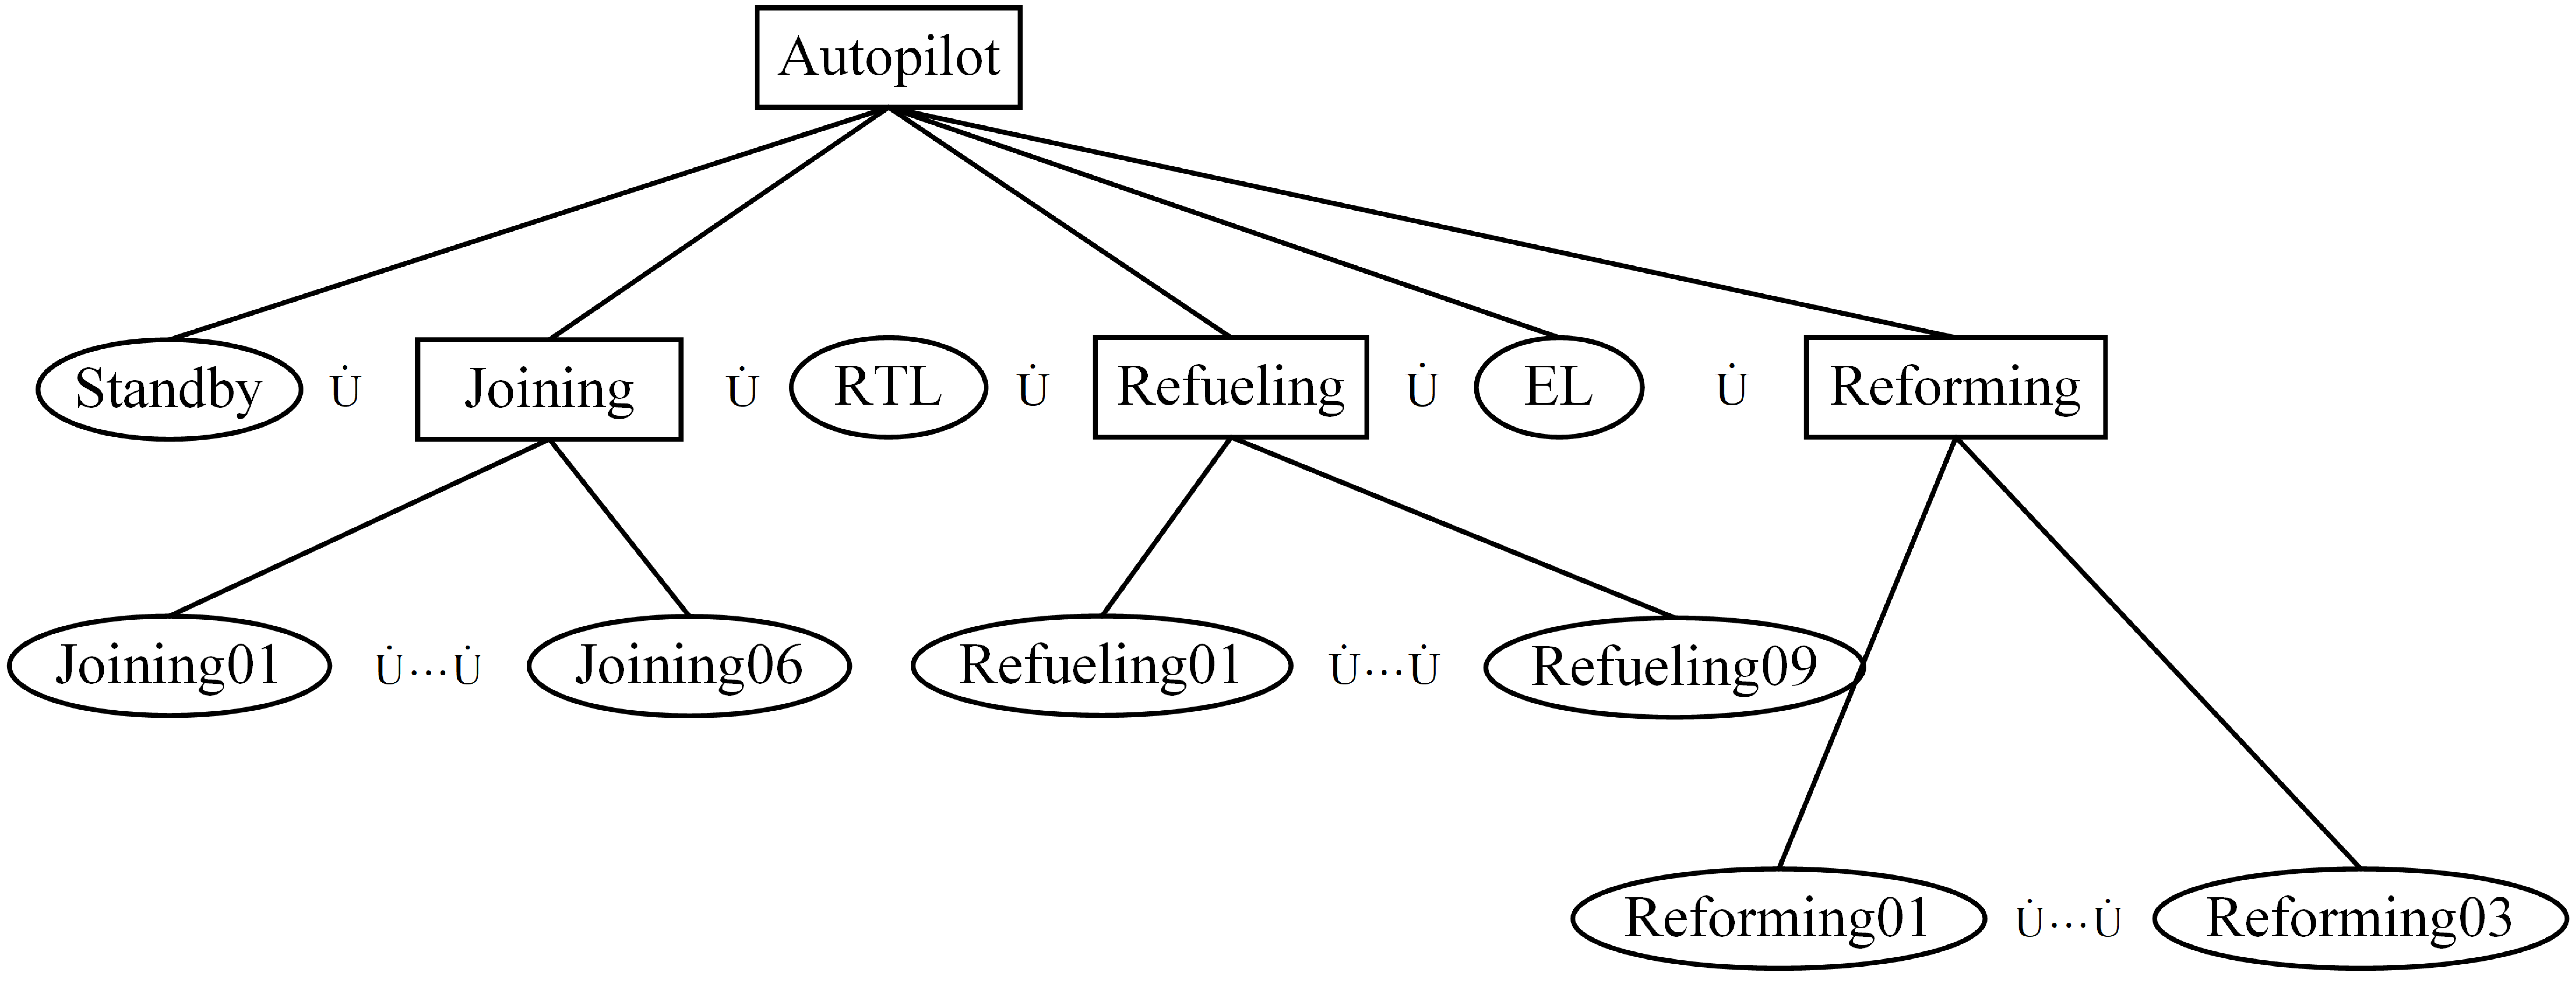
\includegraphics[width=0.8\textwidth]{Figures/Figs_Ch14/Fig11_SAutopilot}
		\par\end{center}
	\caption{The state tree of \textit{Autopilot}. \textit{Joining01}\ldots\textit{Joining06} are children (OR components) of superstate \textit{Joining}, whose detailed information is shown in Fig. \ref{fig:plantjoi}. It is the same for \textit{Refueling} and \textit{Reforming}, whose information is shown in Fig. \ref{fig:plantref} and Fig. \ref{fig:plantreforming} respectively.}
	\label{fig:staut} 
\end{figure}

\begin{figure}[h]
	\begin{center}
		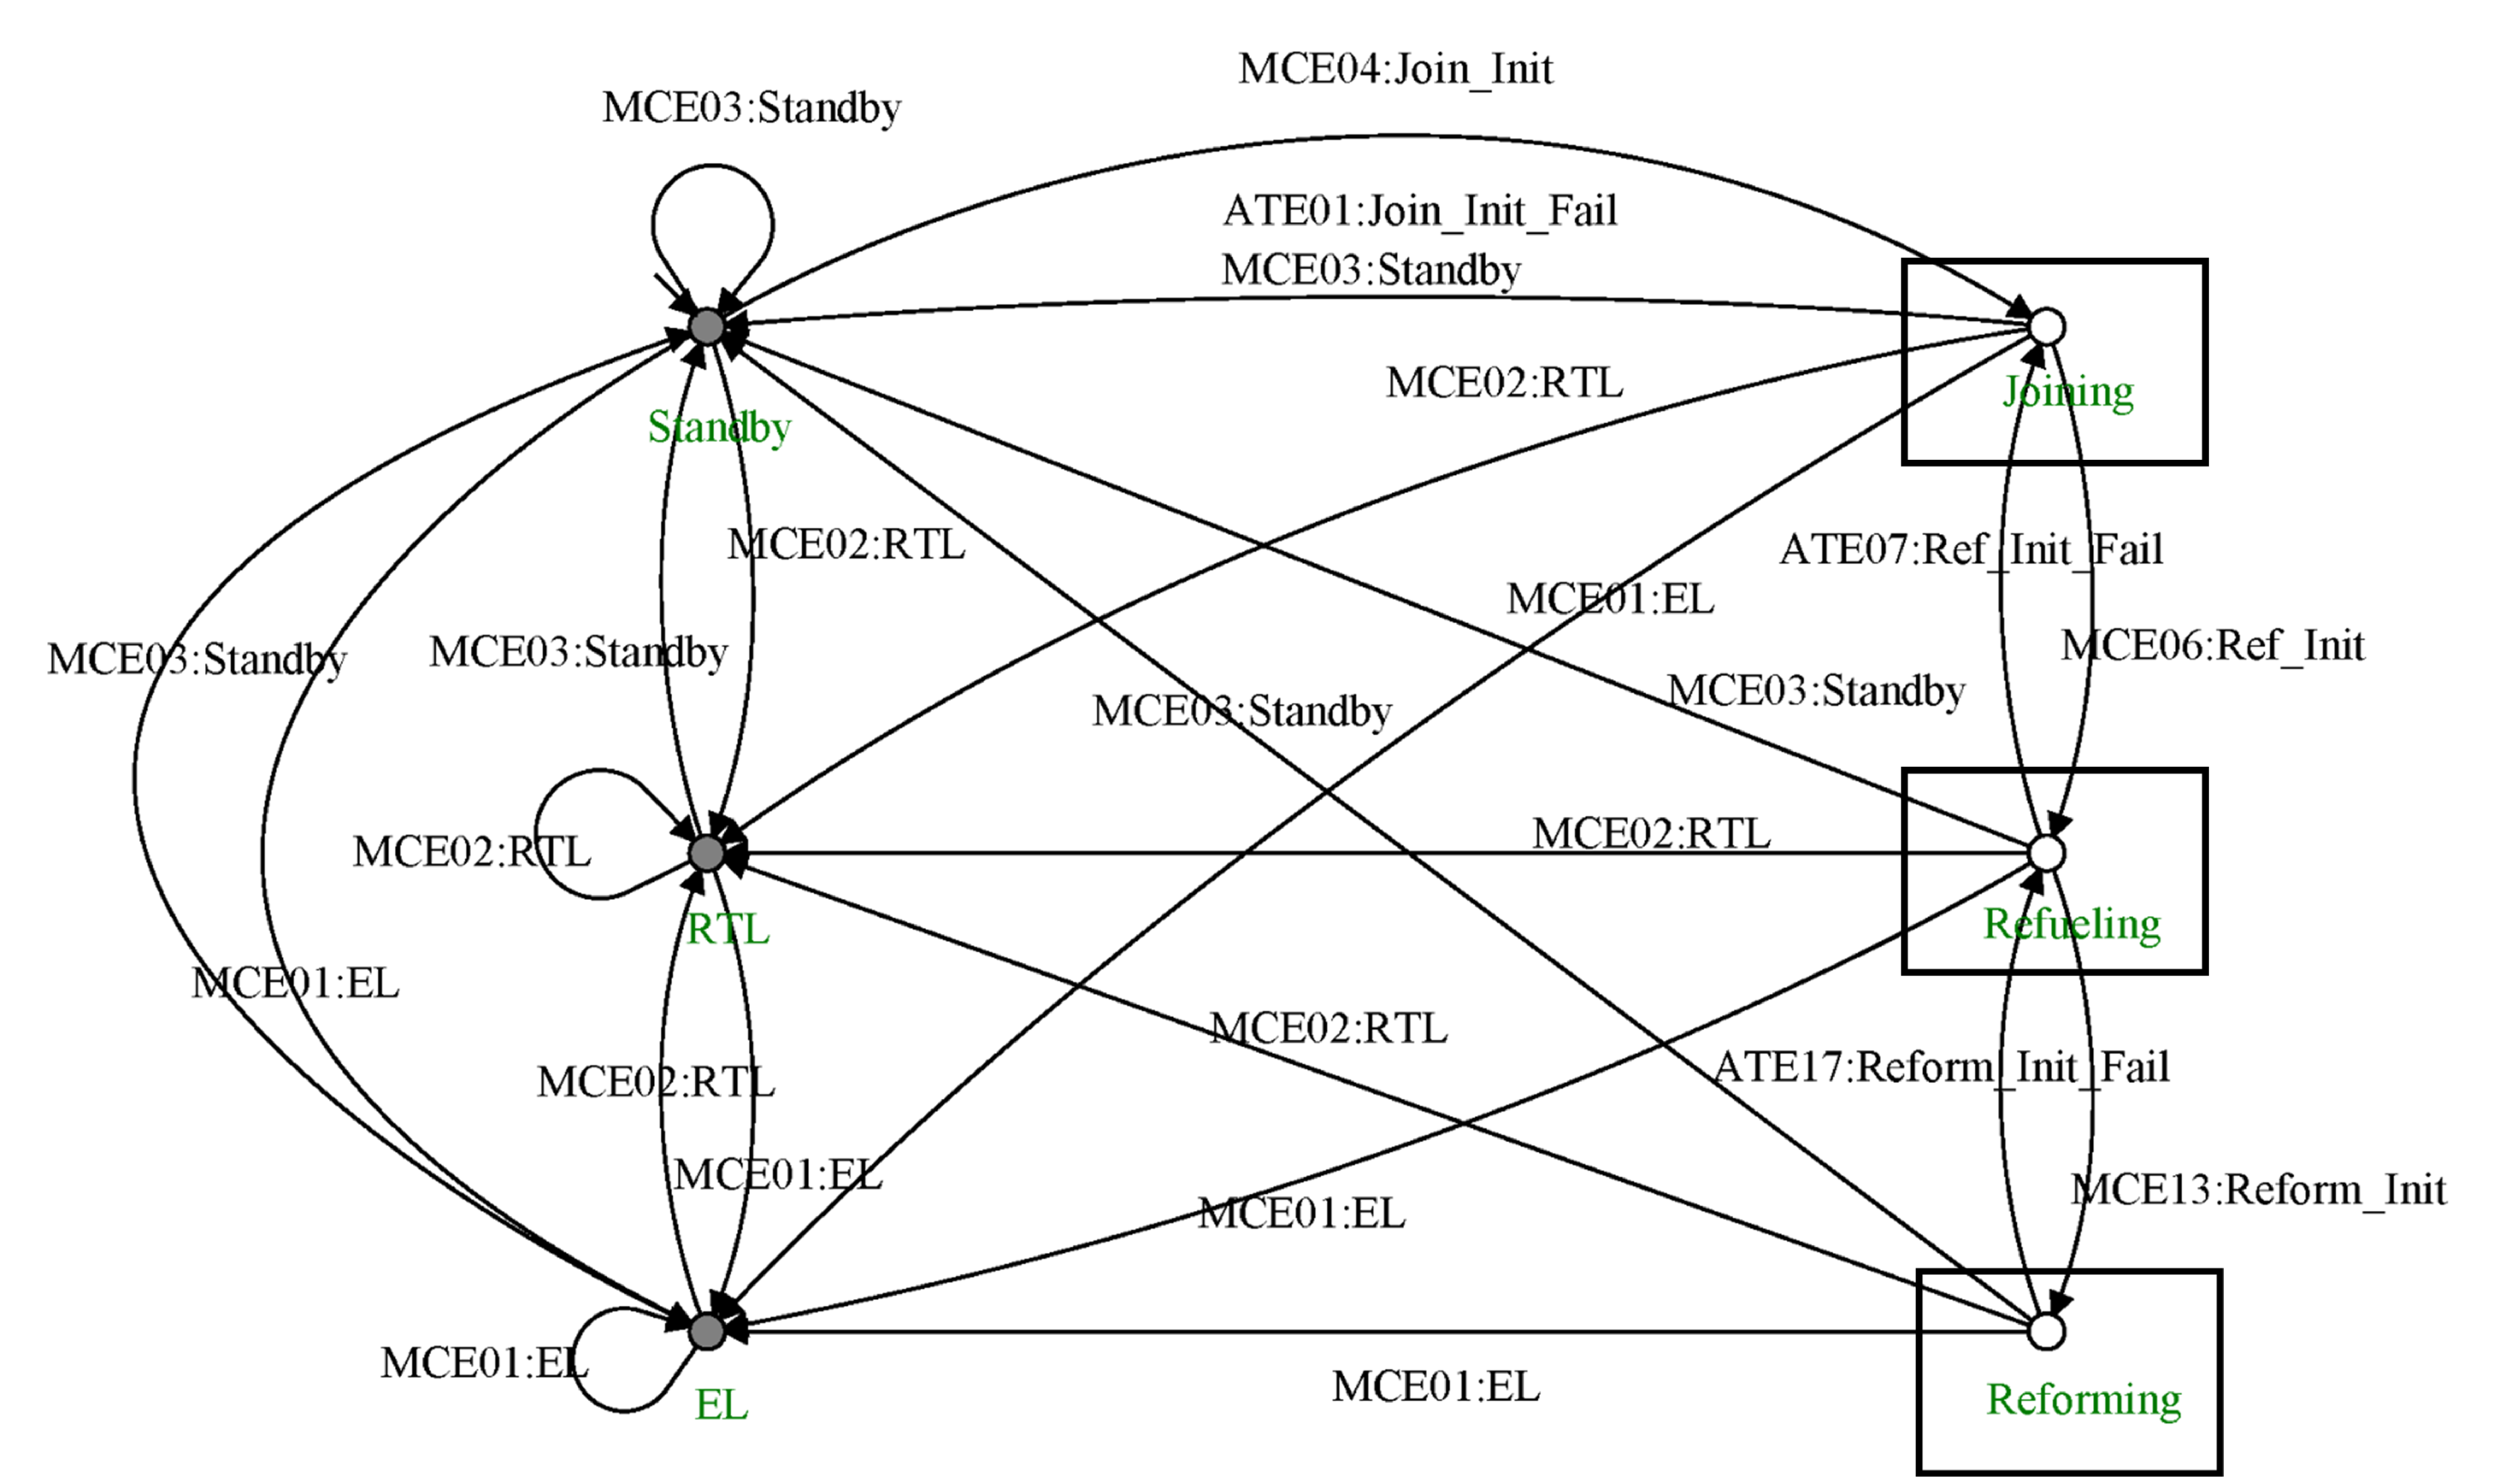
\includegraphics[width=0.8\textwidth]{Figures/Figs_Ch14/Fig12_HAutopilot}
		\par\end{center}
	\caption{The holon of \textit{Autopilot}. Figures are plotted through SUPREMICA \cite{akesson2003supremica}. Note that circles with arrow pointing to are initial states like \textit{Standby}, and gray circles are marker states like \textit{RTL}. The black squares indicate superstates.}
	\label{fig:holonaut} 
\end{figure}


a) \textit{Joining} superstate:
This is an OR superstate as shown in Fig. \ref{fig:plantjoi}. It corresponds to the joining sub-phase presented in section \ref{sec:mode_decom}, and contains six simple states.

When MCE04 happens, the \textit{Autopilot} enters \textit{Joining} superstate from \textit{Standby}, and stays in \textit{Joining01} state (belonging to JOINING-INIT MODE). When this maneuver succeeds (``ATE02:Join-Init-Succ"), it enters \textit{Joining02} state (belonging to JOINING-WAIT MODE), where the receiver has to wait for the connection clearance from the tanker (FD4, see Table \ref{tab:functiondemand}). When it is not cleared (``ATE03:Join-Connection-no"), the receiver has to check whether the waiting time exceeds the specified threshold (SR5, see Table \ref{tab:safetyreq}). If so, it has to abandon the current AAR task and return to the withdrawal phase. Otherwise, it can keep waiting (MCE05)  or retreat to the withdrawal phase according to its health conditions. Once the receiver is cleared for connection (``ATE04:Join-Connection-yes"), it has to check whether it satisfies the safety requirement for MCE06 (SR6, see Table \ref{tab:safetyreq}). If  satisfied, the receiver can execute the event MCE06. Otherwise, it has to wait or withdraw. 



b) \textit{Refueling} superstate: This is an OR superstate as shown in Fig. \ref{fig:plantref}. It corresponds to the Refueling sub-phase, and contains nine simple states. 

Event MCE06 brings the \textit{Autopilot} from \textit{Joining} to \textit{Refueling} superstate. In the \textit{Refueling02} state (belonging to REFUELING-CAPTURE MODE), according to the safety requirement (SR7), the receiver can choose to initiate a connection (MCE08), back to \textit{Refueling01} state (MCE07) or back to the withdrawal phase. MCE09 is the substitute for MCE08, so that the pilot can use it to force the connection action when MCE08 is forbidden by the generated supervisor (FD6). The connection action has two results: ``ATE09:Ref-Cap-Fail" and ``ATE10:Ref-Cap-Succ". Failure brings the receiver back to the  \textit{Refueling02} state while success leads the receiver to the \textit{Refueling04} state (belonging to REFUELING-TRANSFER MODE), whose transitions are similar to those of \textit{Refueling02} state.	

Success of fuel transfer leads the receiver to \textit{Refueling06} state, where it has to wait for the disconnection clearance (FD4). If not cleared, the receiver has to check the waiting time (SR9), similar to \textit{Joining02} state. But if the time runs out, the receiver will directly disconnect with the tanker instead of returning to the withdrawal phase. If cleared, the receiver can initiate the event MCE13 or return to the withdrawal phase.

\begin{figure}[h]
	\begin{center}
		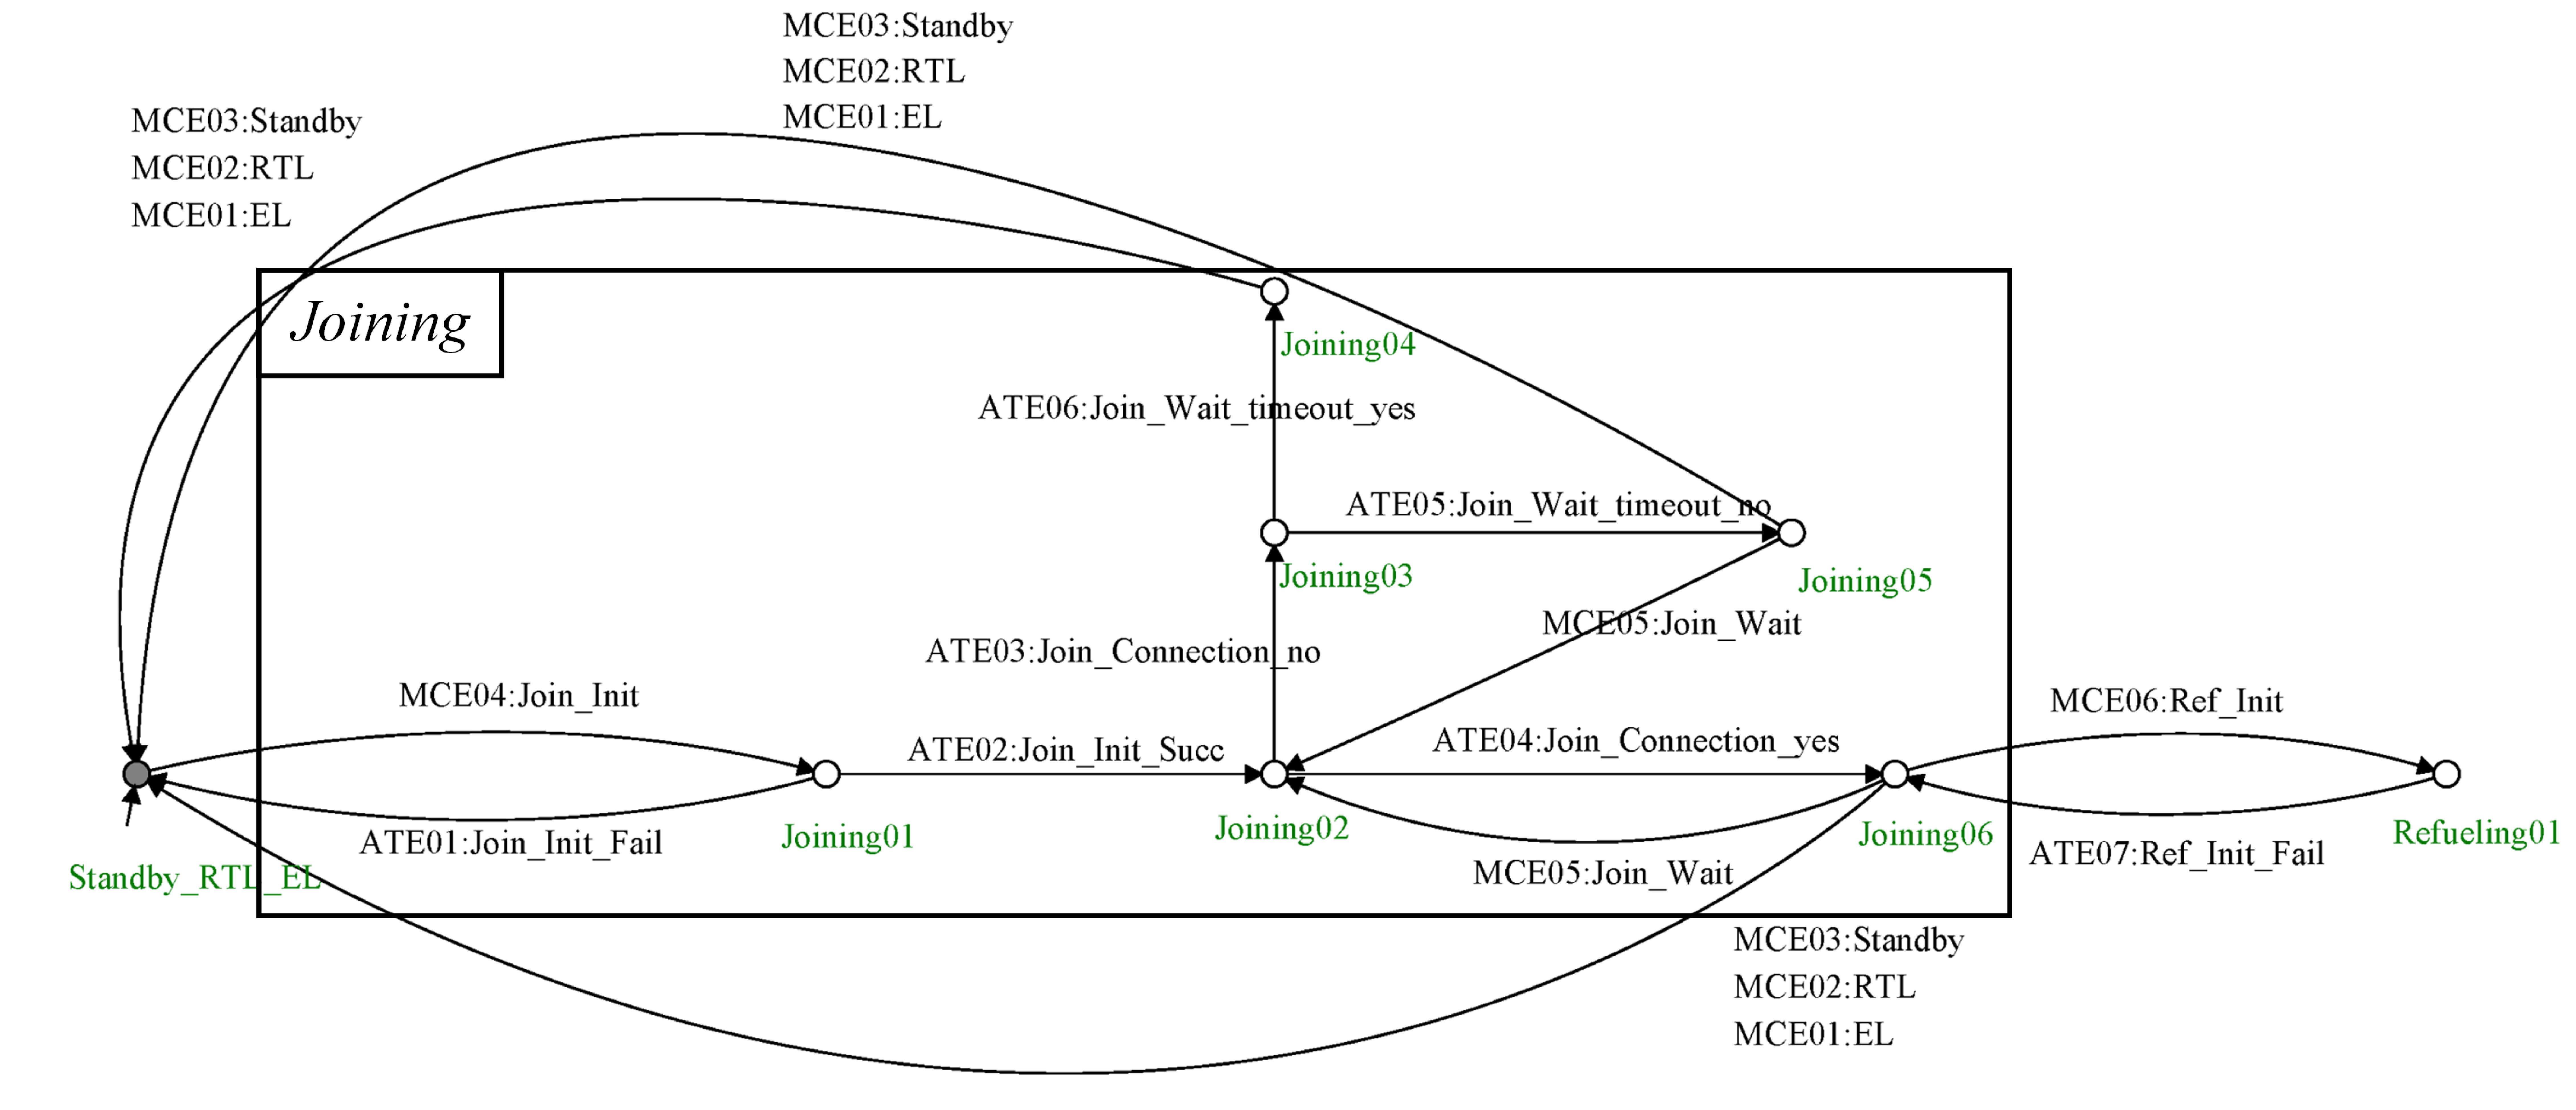
\includegraphics[width=0.8\textwidth]{Figures/Figs_Ch14/Fig13_HJoining}
		\par\end{center}
	\caption{The holon of \textit{Joining}. The simple states and transitions inside superstate \textit{Joining} are enclosed by the black square. To avoid messy transition lines, this diagram has been simplified by using node \textit{Standby\_RTL\_EL} to represent three separate nodes including \textit{Standby}, \textit{RTL} and \textit{EL}, which have the same transition lines from node \textit{Joining04}, \textit{Joining05}, and \textit{Joining06}. The following two diagrams have been simplified as well.}
	\label{fig:plantjoi} 
\end{figure}

\begin{figure}[h]
	\begin{center}
		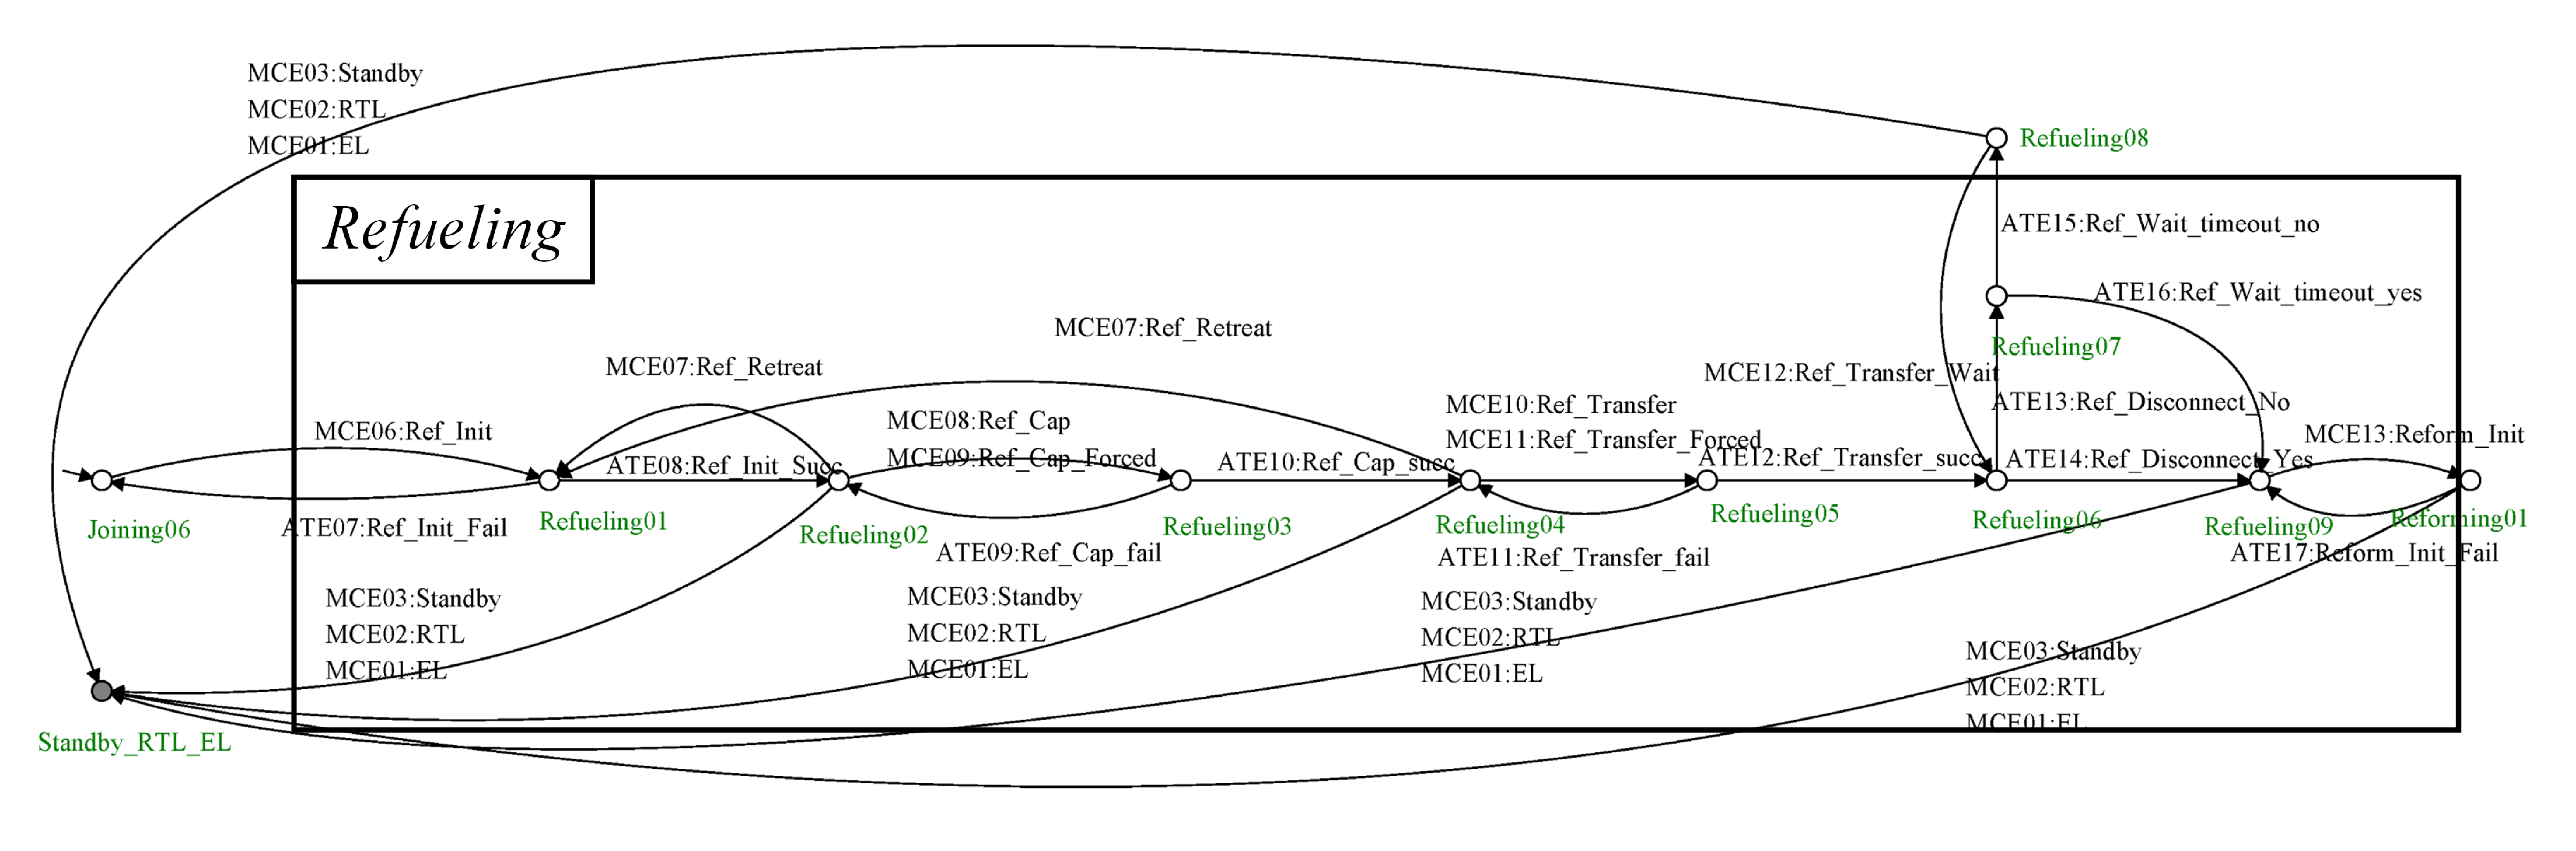
\includegraphics[width=1\textwidth]{Figures/Figs_Ch14/Fig14_HRefueling}
		\par\end{center}
	\caption{The holon of \textit{Refueling}.}
	\label{fig:plantref} 
\end{figure}

\begin{figure}[h]
	\begin{center}
		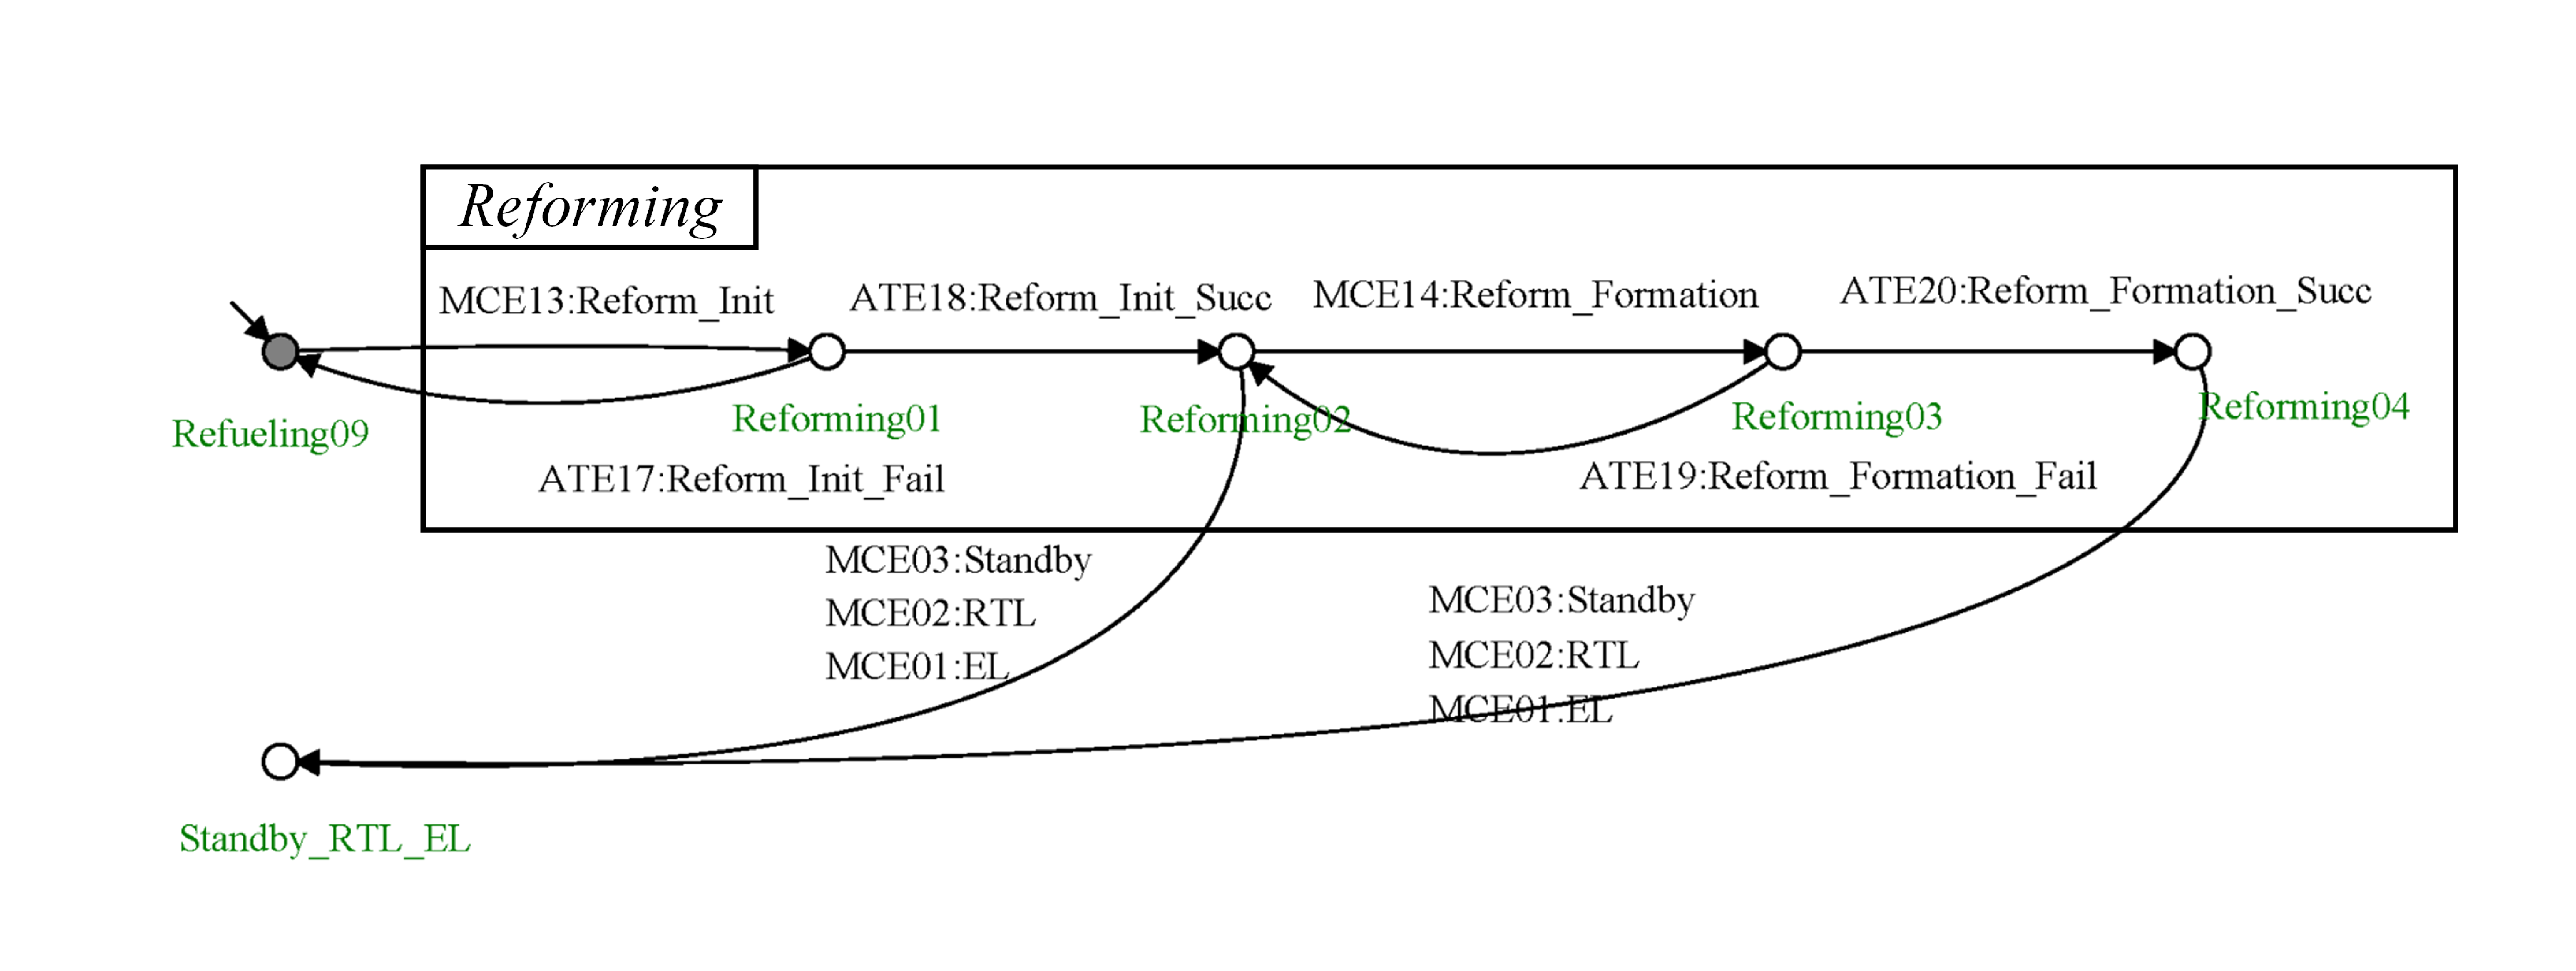
\includegraphics[width=1\textwidth]{Figures/Figs_Ch14/Fig15_HReform}
		\par\end{center}
	\caption{The holon of \textit{Reforming}.}
	\label{fig:plantreforming} 
\end{figure}


c) \textit{Reforming} superstate: This is an OR superstate as shown in Fig. \ref{fig:plantreforming}. It corresponds to the Reforming sub-phase, and contains three simple states.  MCE13 will bring the receiver from \textit{Refueling} to the \textit{Reforming} superstate. Its success will lead to the \textit{Reforming02} state, where the receiver can return to the withdrawal phase due to health conditions or form the formation (MCE14). Event ``ATE20:Reform-Formation-Succ" implies the completion of a work cycle of AAR, and then the receiver should return to the withdrawal phase.

\subsubsection{(Receiver) Subsystem}
\textit{Subsystem} is another AND component of Receiver, working in parallel with \textit{Autopilot}. This  superstate is responsible for recording the health information of different subsystems, namely Navigation, Control, Fuel, Engine, Drogue\&probe, Datalink and Tanker safety subsystems. Their state trees are shown in Fig. \ref{fig:stsubsystem}. Their holon structures are similar to Fig. \ref{fig:failure-automaton} and \ref{fig:fuelfailureautomation}. The holons for \textit{Navigation} and \textit{Fuel} superstates are shown in Fig. \ref{fig:plantnavi} and \ref{fig:plantfuel} as an example.

\begin{figure}[h]
	\begin{center}
		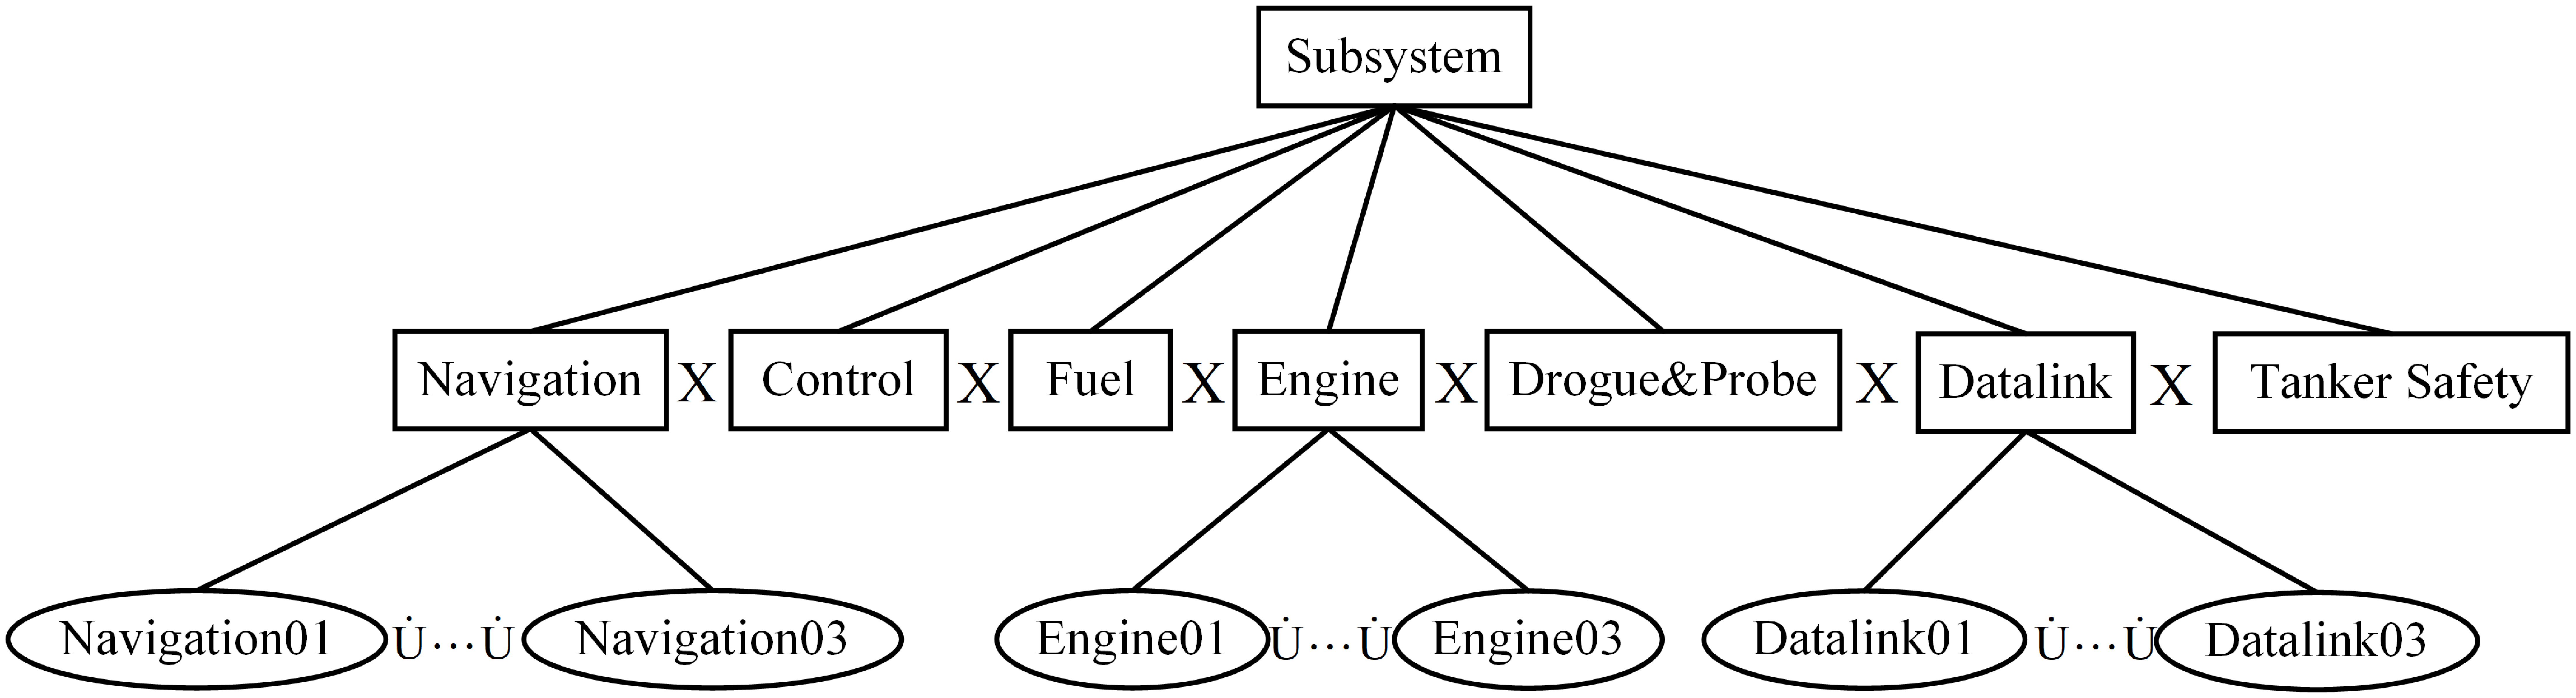
\includegraphics[width=0.8\textwidth]{Figures/Figs_Ch14/Fig16_SSubsystem}
		\par\end{center}
	\caption{The state tree of \textit{Subsystem}. Only part of the simple states are presented here owing to limited pages. These simple states represent different health conditions. For example, \textit{Navigation01} means \textit{normal}, \textit{Navigation02} means \textit{minor damage}, and \textit{Navigation03} means \textit{critical damage}.}
	\label{fig:stsubsystem} 
\end{figure}
\begin{figure}[h]
	\begin{center}
		\includegraphics[width=0.7\textwidth]{Figures/Figs_Ch14/Fig17a_HNavigation}
		\par\end{center}
	\caption{The holon of \textit{Navigation} superstate.}
	\label{fig:plantnavi} 
\end{figure}	
\begin{figure}[h]
	\begin{center}
		\includegraphics[width=0.7\textwidth]{Figures/Figs_Ch14/Fig17b_HFuel}
		\par\end{center}
	\caption{The holon of \textit{Fuel} superstate.}
	\label{fig:plantfuel} 
\end{figure}


\subsubsection{(Pilot) Withdrawal}
\textit{Withdrawal} is an AND component of \textit{Pilot}, which is responsible for implementing the FD7 in Table \ref{tab:functiondemand}. Its holon is shown in Fig. \ref{fig:holonwith}. As shown in this figure, when ``MIE02:RTL" happens, i.e., the pilot requires the receiver retreat to RTL MODE, both MCE02 and MCE01 are allowed to happen. This means the receiver can also switch to EL MODE besides RTL MODE in case the receiver is unhealthy and cannot return to base.
\begin{figure}[h]
	\begin{center}
		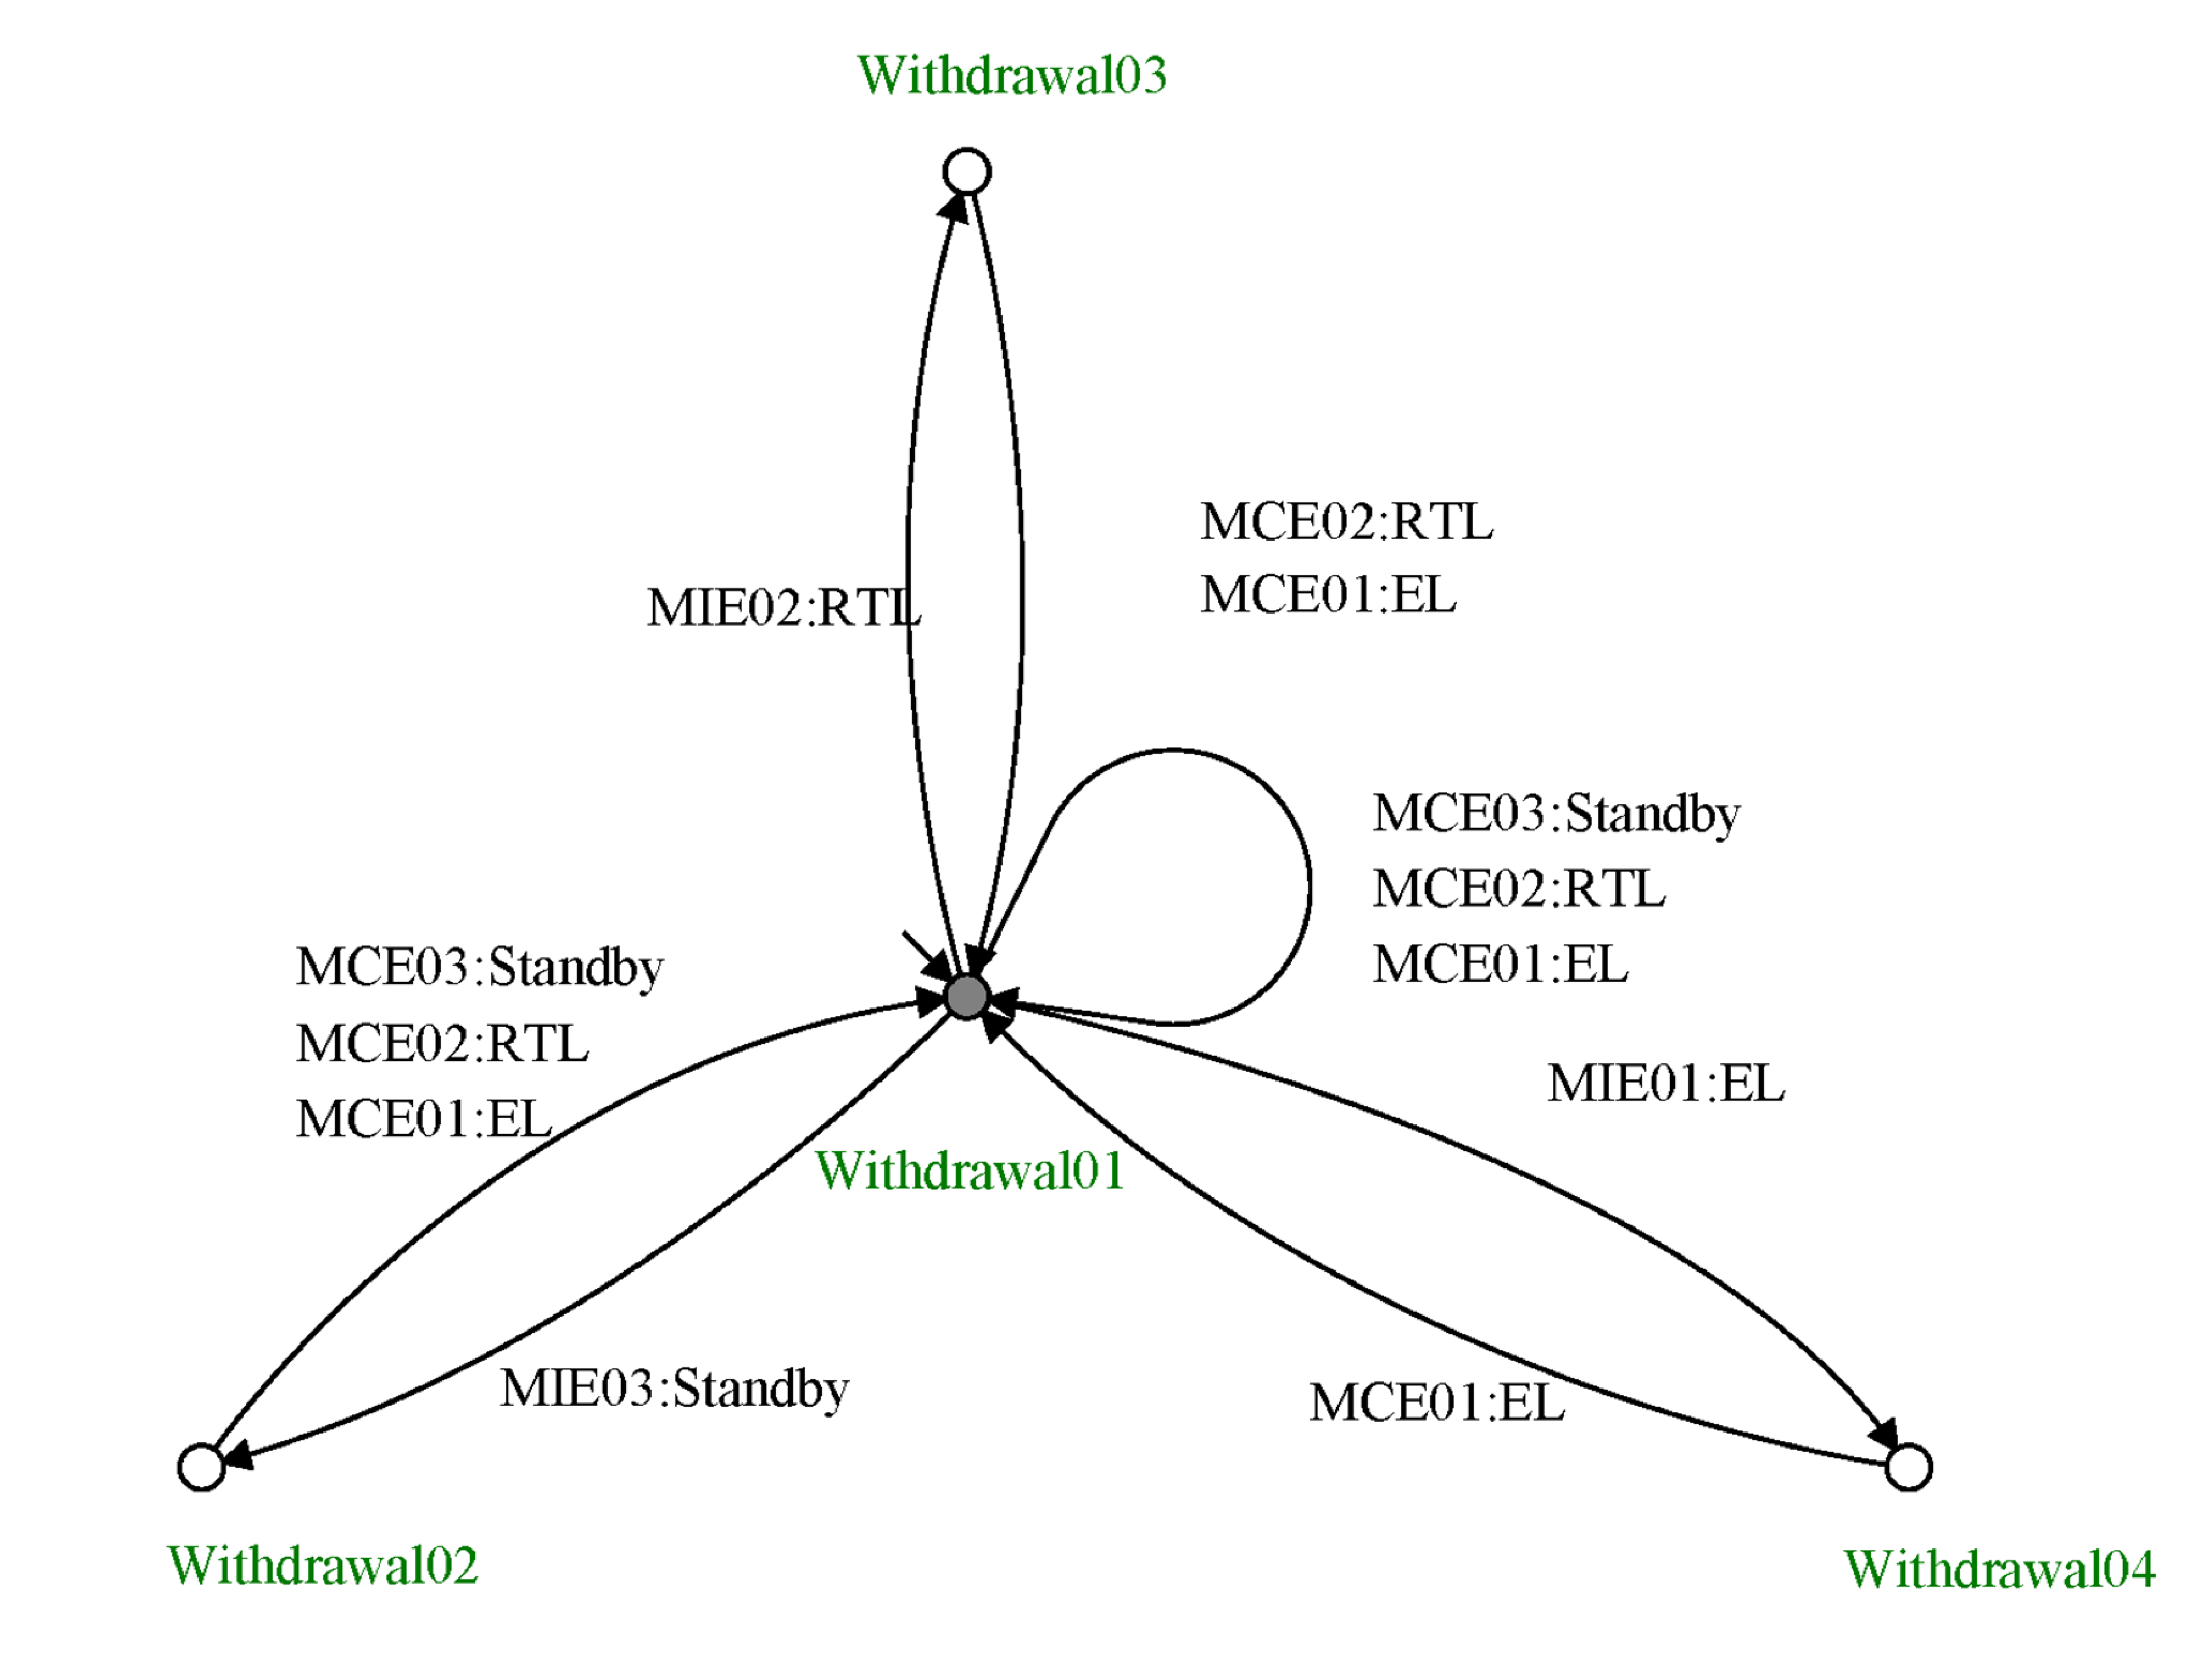
\includegraphics[width=0.6\textwidth]{Figures/Figs_Ch14/Fig18a_HWithdrawal}
		\par\end{center}
	\caption{The holon of \textit{Withdrawal} superstate.}
	\label{fig:holonwith} 
\end{figure}	


\subsubsection{(Pilot) Force}
\textit{Force} is another AND component of \textit{Pilot} and implements the FD6 (in Table \ref{tab:functiondemand}). As shown in Fig. \ref{fig:holonforce}, MCE09, a substitute of MCE08, can only be enabled when ``MIE04:Force-Ref-Cap" happens, i.e., the pilot gives the corresponding command. After MCE09 or MCE08, this holon will return to the original state \textit{Force01}. MCE03 is similar to MCE09.
\begin{figure}[h]
	\begin{center}
		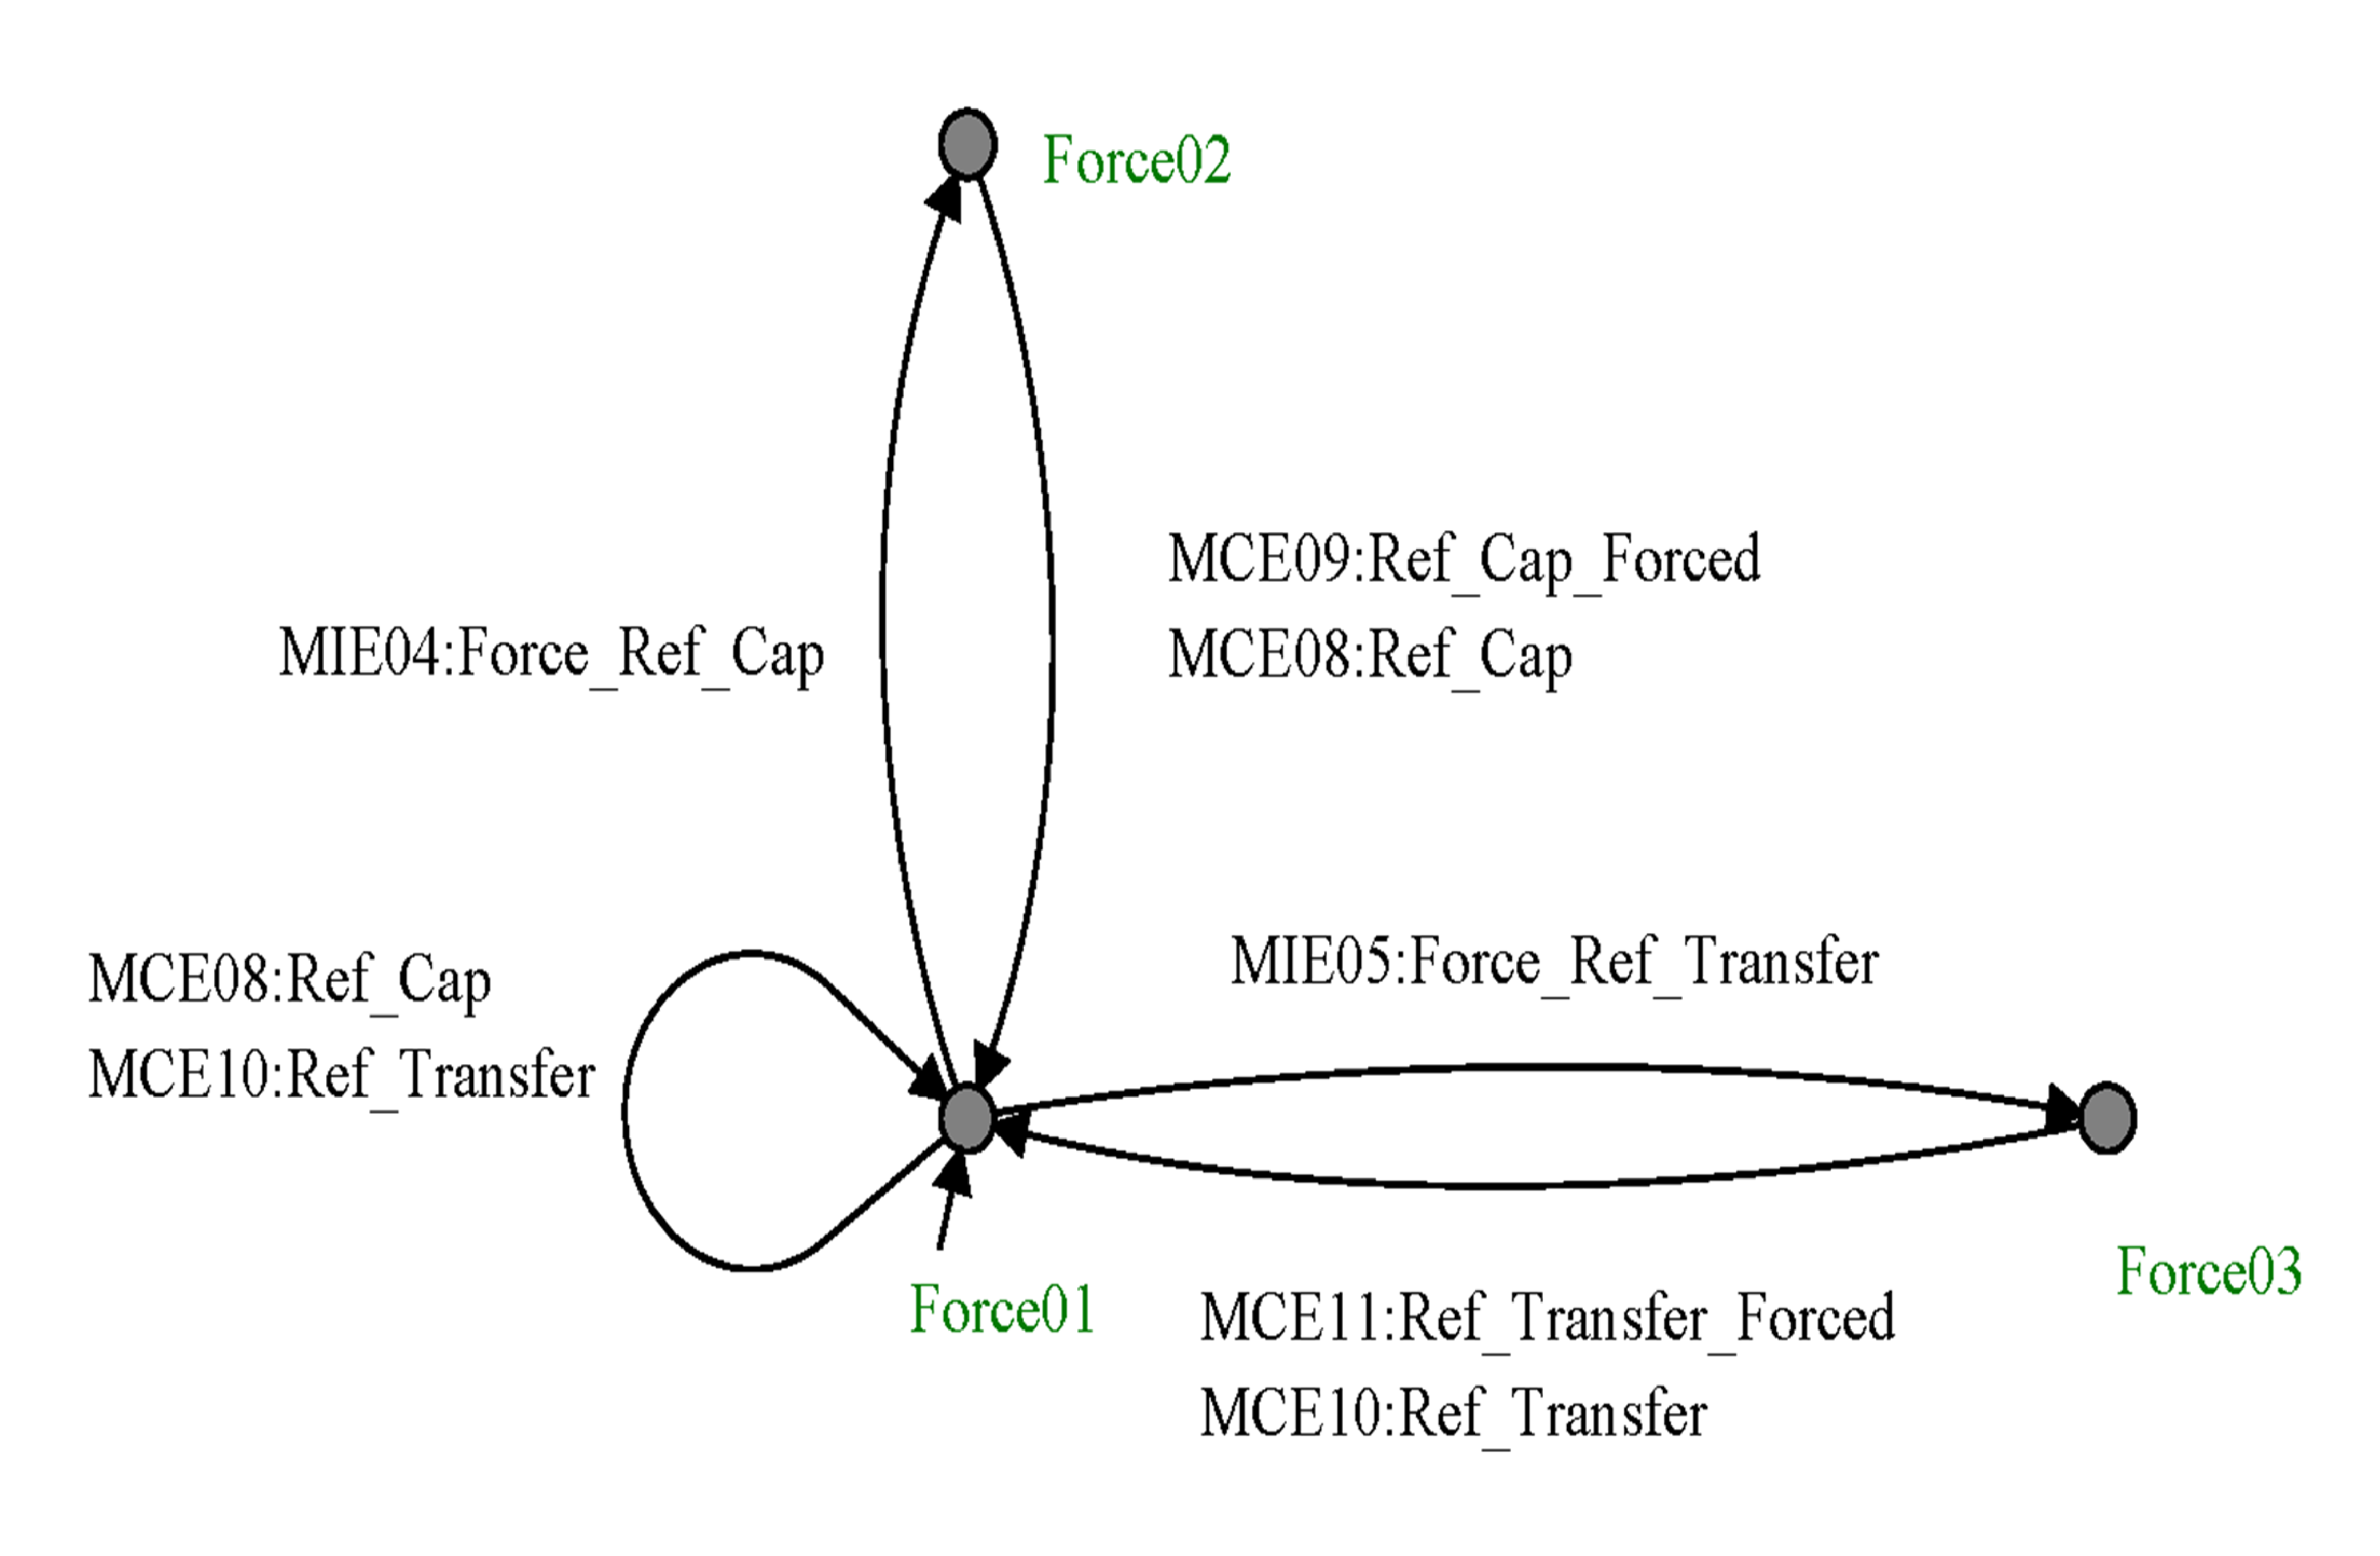
\includegraphics[width=0.6\textwidth]{Figures/Figs_Ch14/Fig18b_HForce}
		\par\end{center}
	\caption{The holon of \textit{Force} superstate.}
	\label{fig:holonforce} 
\end{figure}	


\subsubsection{Plant summary}

So far, all the superstates and simple states of the \textit{Plant} have been introduced, as shown in Fig. \ref{fig:plant}. Recall that the state of superstate depends on states of its children. Therefore the state of \textit{Plant}, namely \textit{Plant State}, can be represented as a 10-tuple \[PS=(x_1, x_2, ..., x_{10})\] where $ x_i $ is the state of the ten superstates in the sequence of \textit{Autopilot}, \textit{Navigation}, \textit{Control}, \textit{Fuel}, \textit{Engine}, \textit{Drogue\&probe}, \textit{Datalink}, \textit{Tankersafety}, \textit{Withdrawal} and \textit{Force}. An example of plant state is $ PS=(RTL, Navigation01,\\ Control01, Fuel01, \allowbreak Engine01,  Drogue\&probe01, Datalink01, Tankersafety02, \allowbreak Withdrawal03, Force03) $, where the meaning of $ Control01, \allowbreak Fuel01,... , Tankersafety02 $ is displayed in Fig. \ref{fig:stsubsystem}.
\begin{figure}[h]
	\begin{center}
		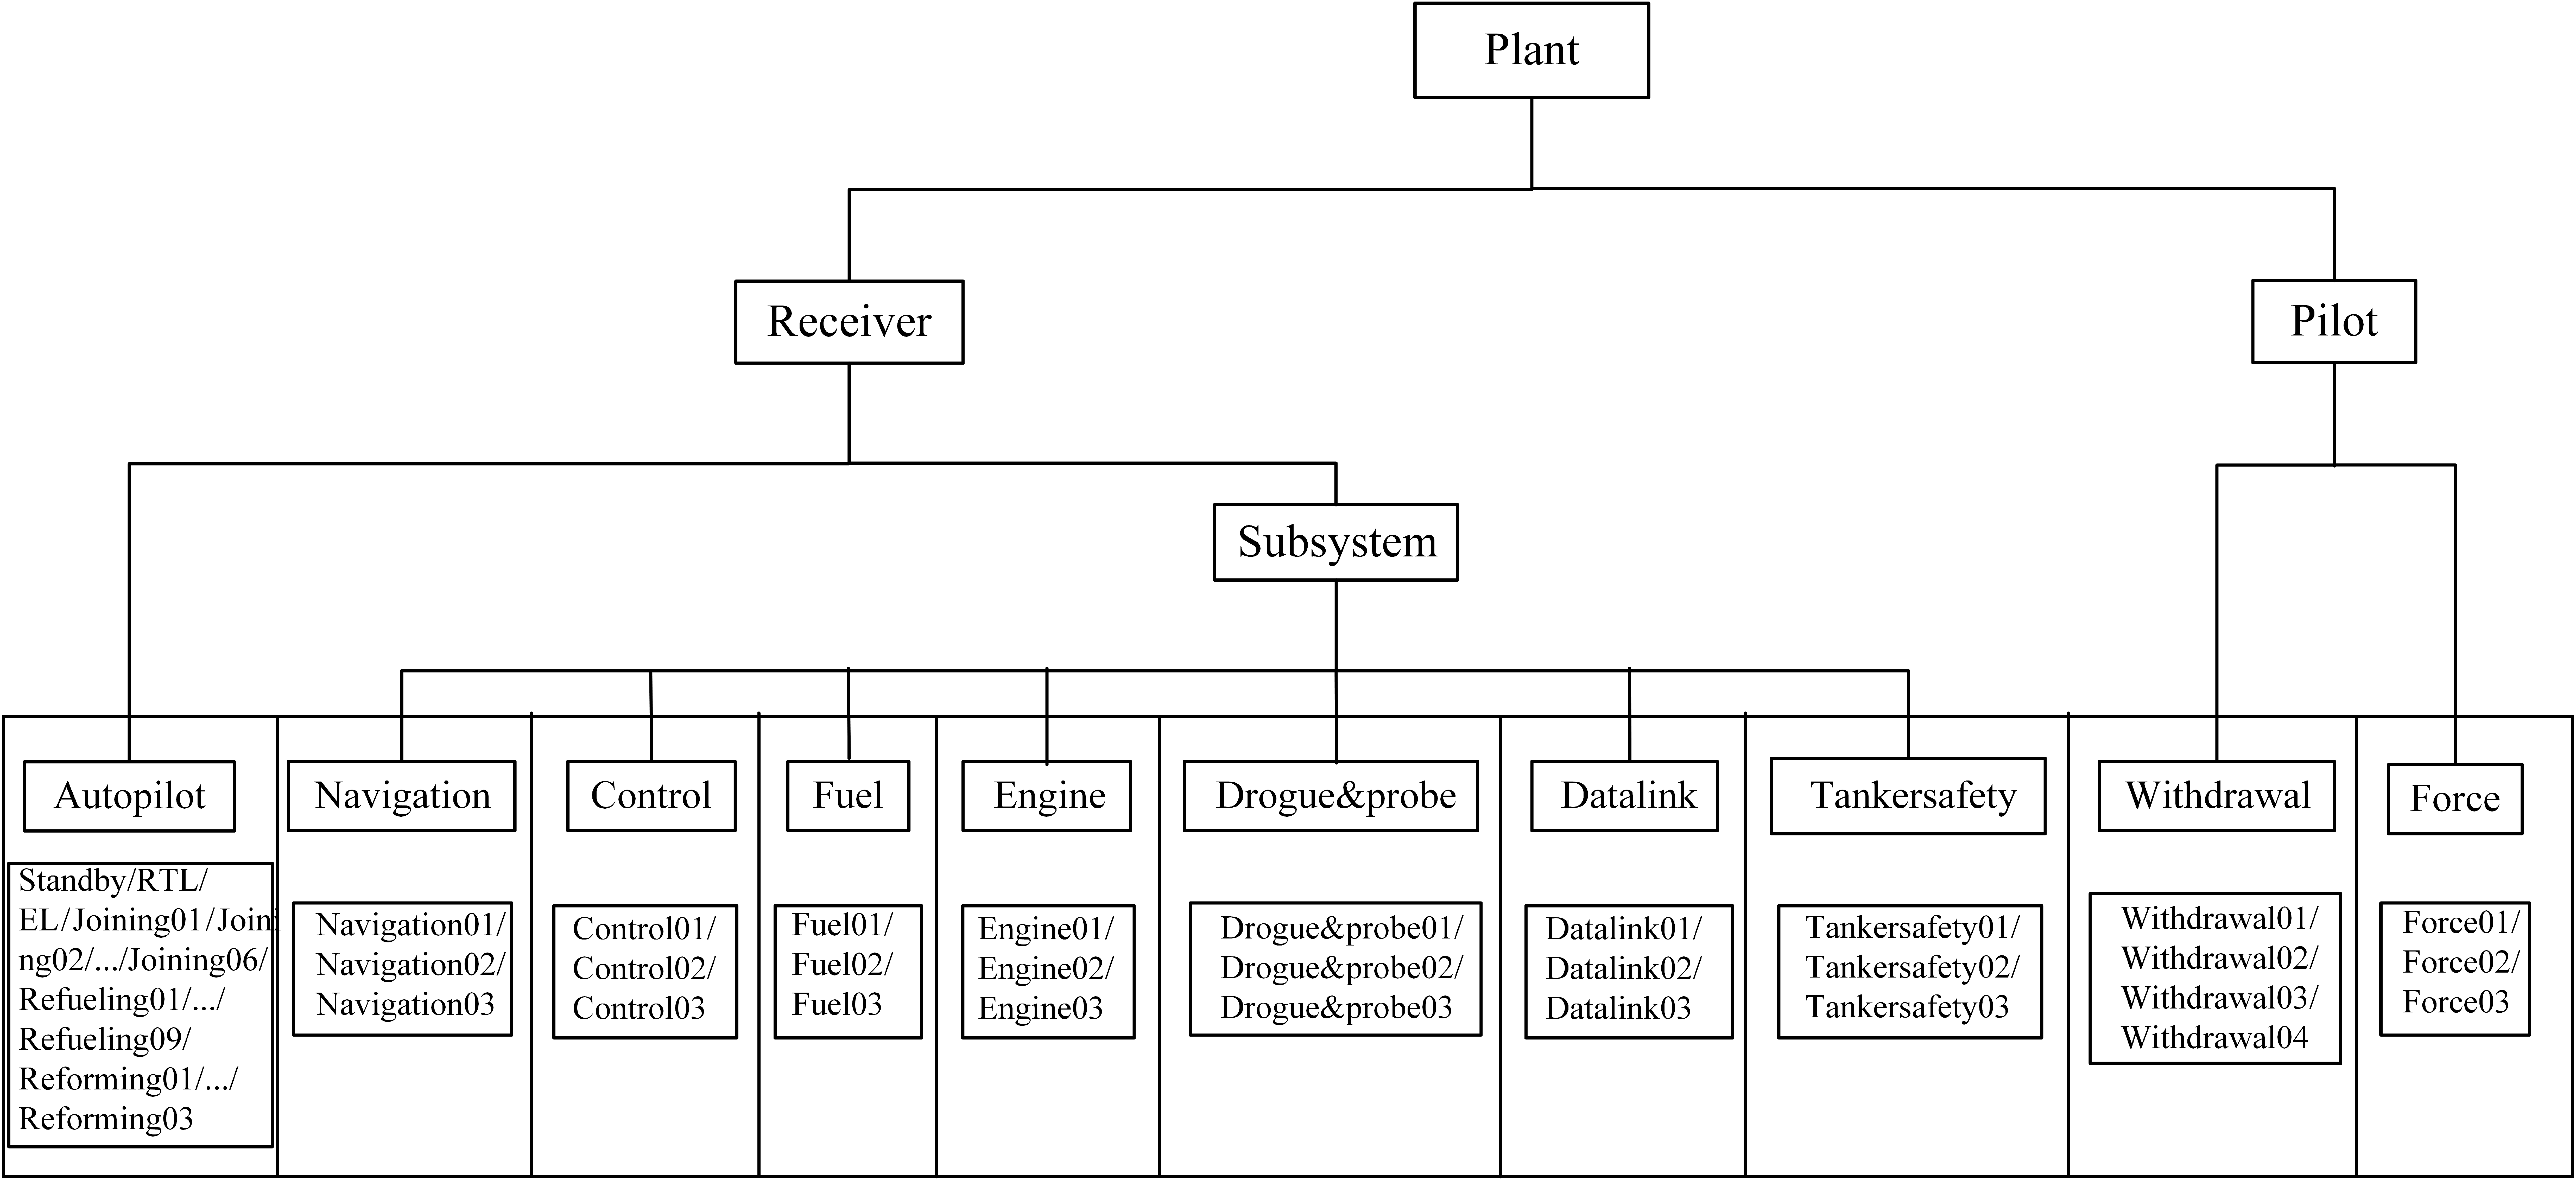
\includegraphics[width=0.9\textwidth]{Figures/Figs_Ch14/Fig19_PlantOverview}
		\par\end{center}
	\caption{Plant overview.}
	\label{fig:plant} 
\end{figure}	


\subsection{Specification design}
Specifications are mainly used to implement the safety requirements, restricting the undesired and unsafe behaviors of the  system. As stated in section \ref{sec:pss}, these parallel specifications eliminate, in a minimally restrictive fashion, all behaviors leading to blocking states. They can be divided into two categories, including subsystem-related and pilot-related,  as introduced in the following.

\subsubsection{Subsystem-related specifications}
These specifications, including \textit{Spec-Navigation}, \textit{Spec-Control}, \textit{Spec-Fuel}, \textit{Spec-Engine}, \textit{Spec-Drogue\&probe}, \textit{Spec-Datalink} and \textit{Spec-Tankersafety}? are used to restrict system behaviors when certain subsystems are damaged or break down according to the requirements presented in Table \ref{tab:safetyreq}.

Take the \textit{Spec-Navigation} as example. According to SR3 and SR7, when ``SFE01:\allowbreak Navigation-suspension" happens, MCE04, MCE08 and MCE10 should be disabled. Therefore, as shown in Fig. \ref{fig:specnavi}, event sequences including (SFE01, MCE04), (SFE01, MCE08) and (SFE01, MCE10) will lead \textit{Spec-Navigation} into blocking state \textit{SpecNavi99}. And according to all safety requirements, when ``SFE03:Navigation-breakdown" happens, all MCEs except for MCE01 should be forbidden. This means that when the Navigation subsystem breaks down, the receiver should make an emergency landing.

\subsubsection{Pilot-related specifications}
This part refers to the specification \textit{Spec-pilot}, which is used to implement the priority of pilot commands (MIEs) over the autopilot commands (MCEs), as stated in FD5. That is to say, when MIEs happen, except for MCE01, MCE02 and MCE03, other MCEs should be forbidden. As shown in the Fig. \ref{fig:specpilot}, when ``MIE02: RTL" happens, events such as MCE04 and MCE05 are forbidden. Under this situation, the receiver has to perform corresponding mode transitions MCE02 or MCE01.
\begin{figure}[h]
	\begin{center}
		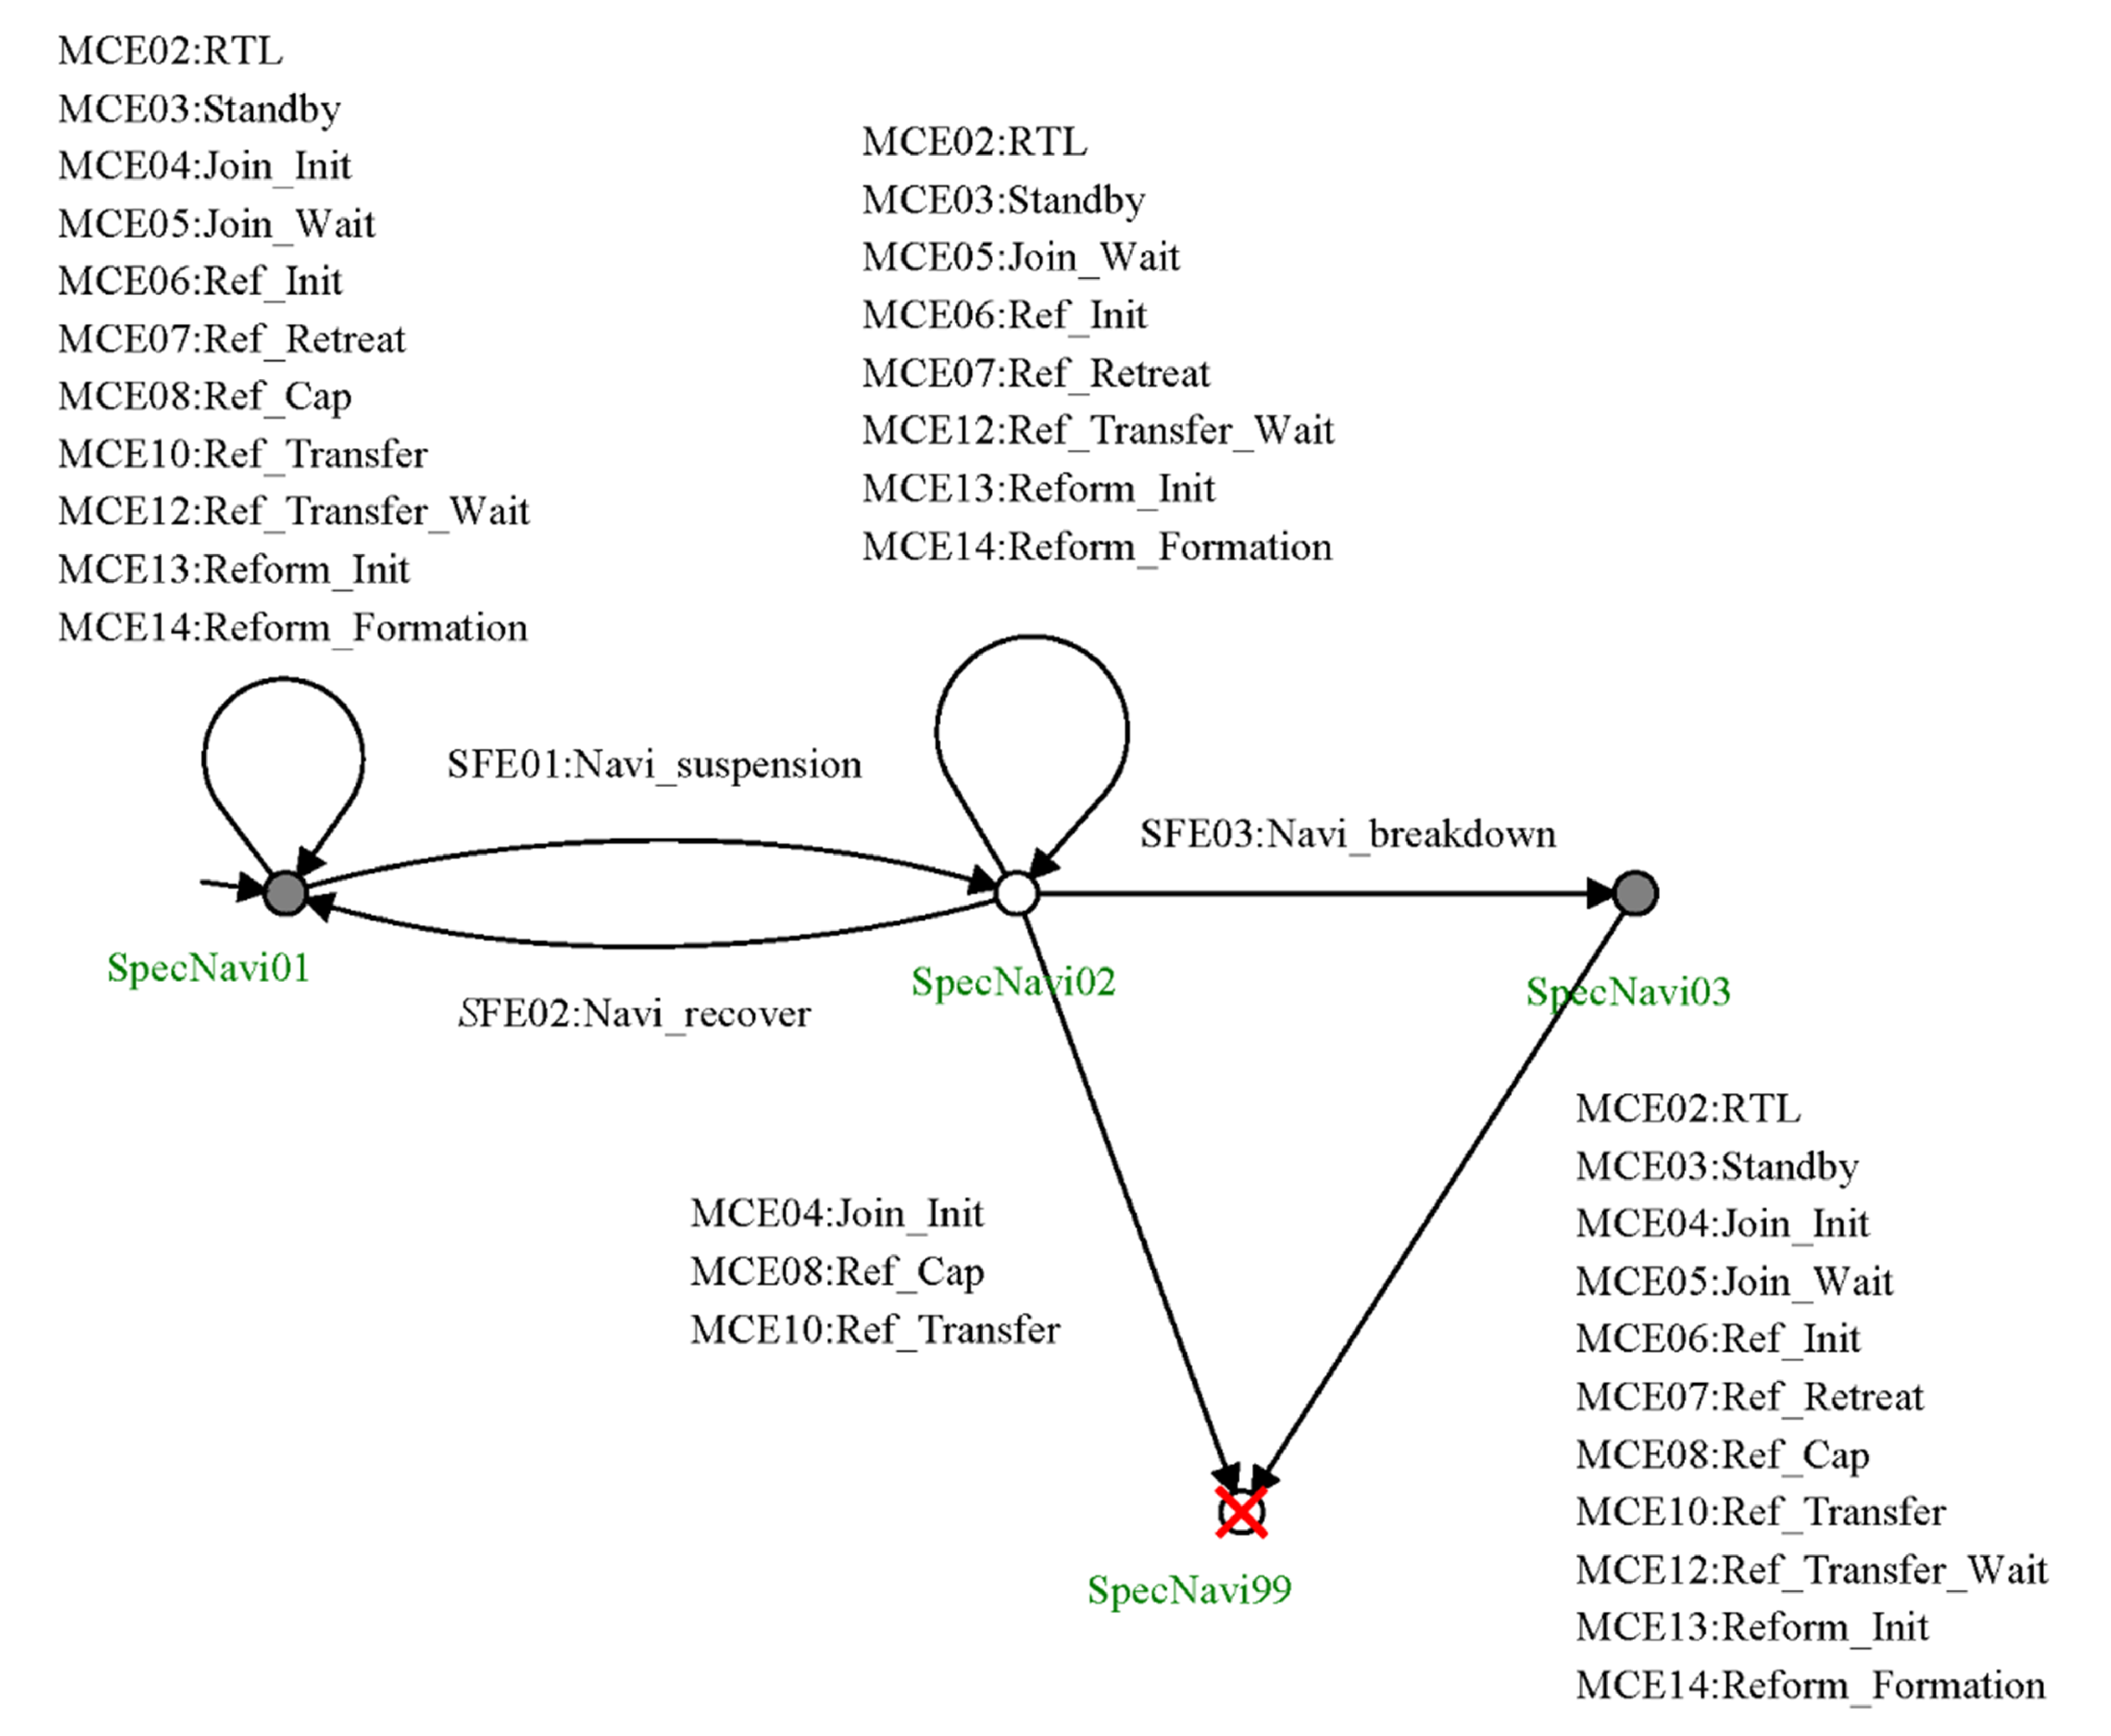
\includegraphics[width=0.9\textwidth]{Figures/Figs_Ch14/Fig20_HSNavi}
		\par\end{center}
	\caption{The holon of \textit{Spec-Navigation}.}
	\label{fig:specnavi} 
\end{figure}
\begin{figure}[h]
	\begin{center}
		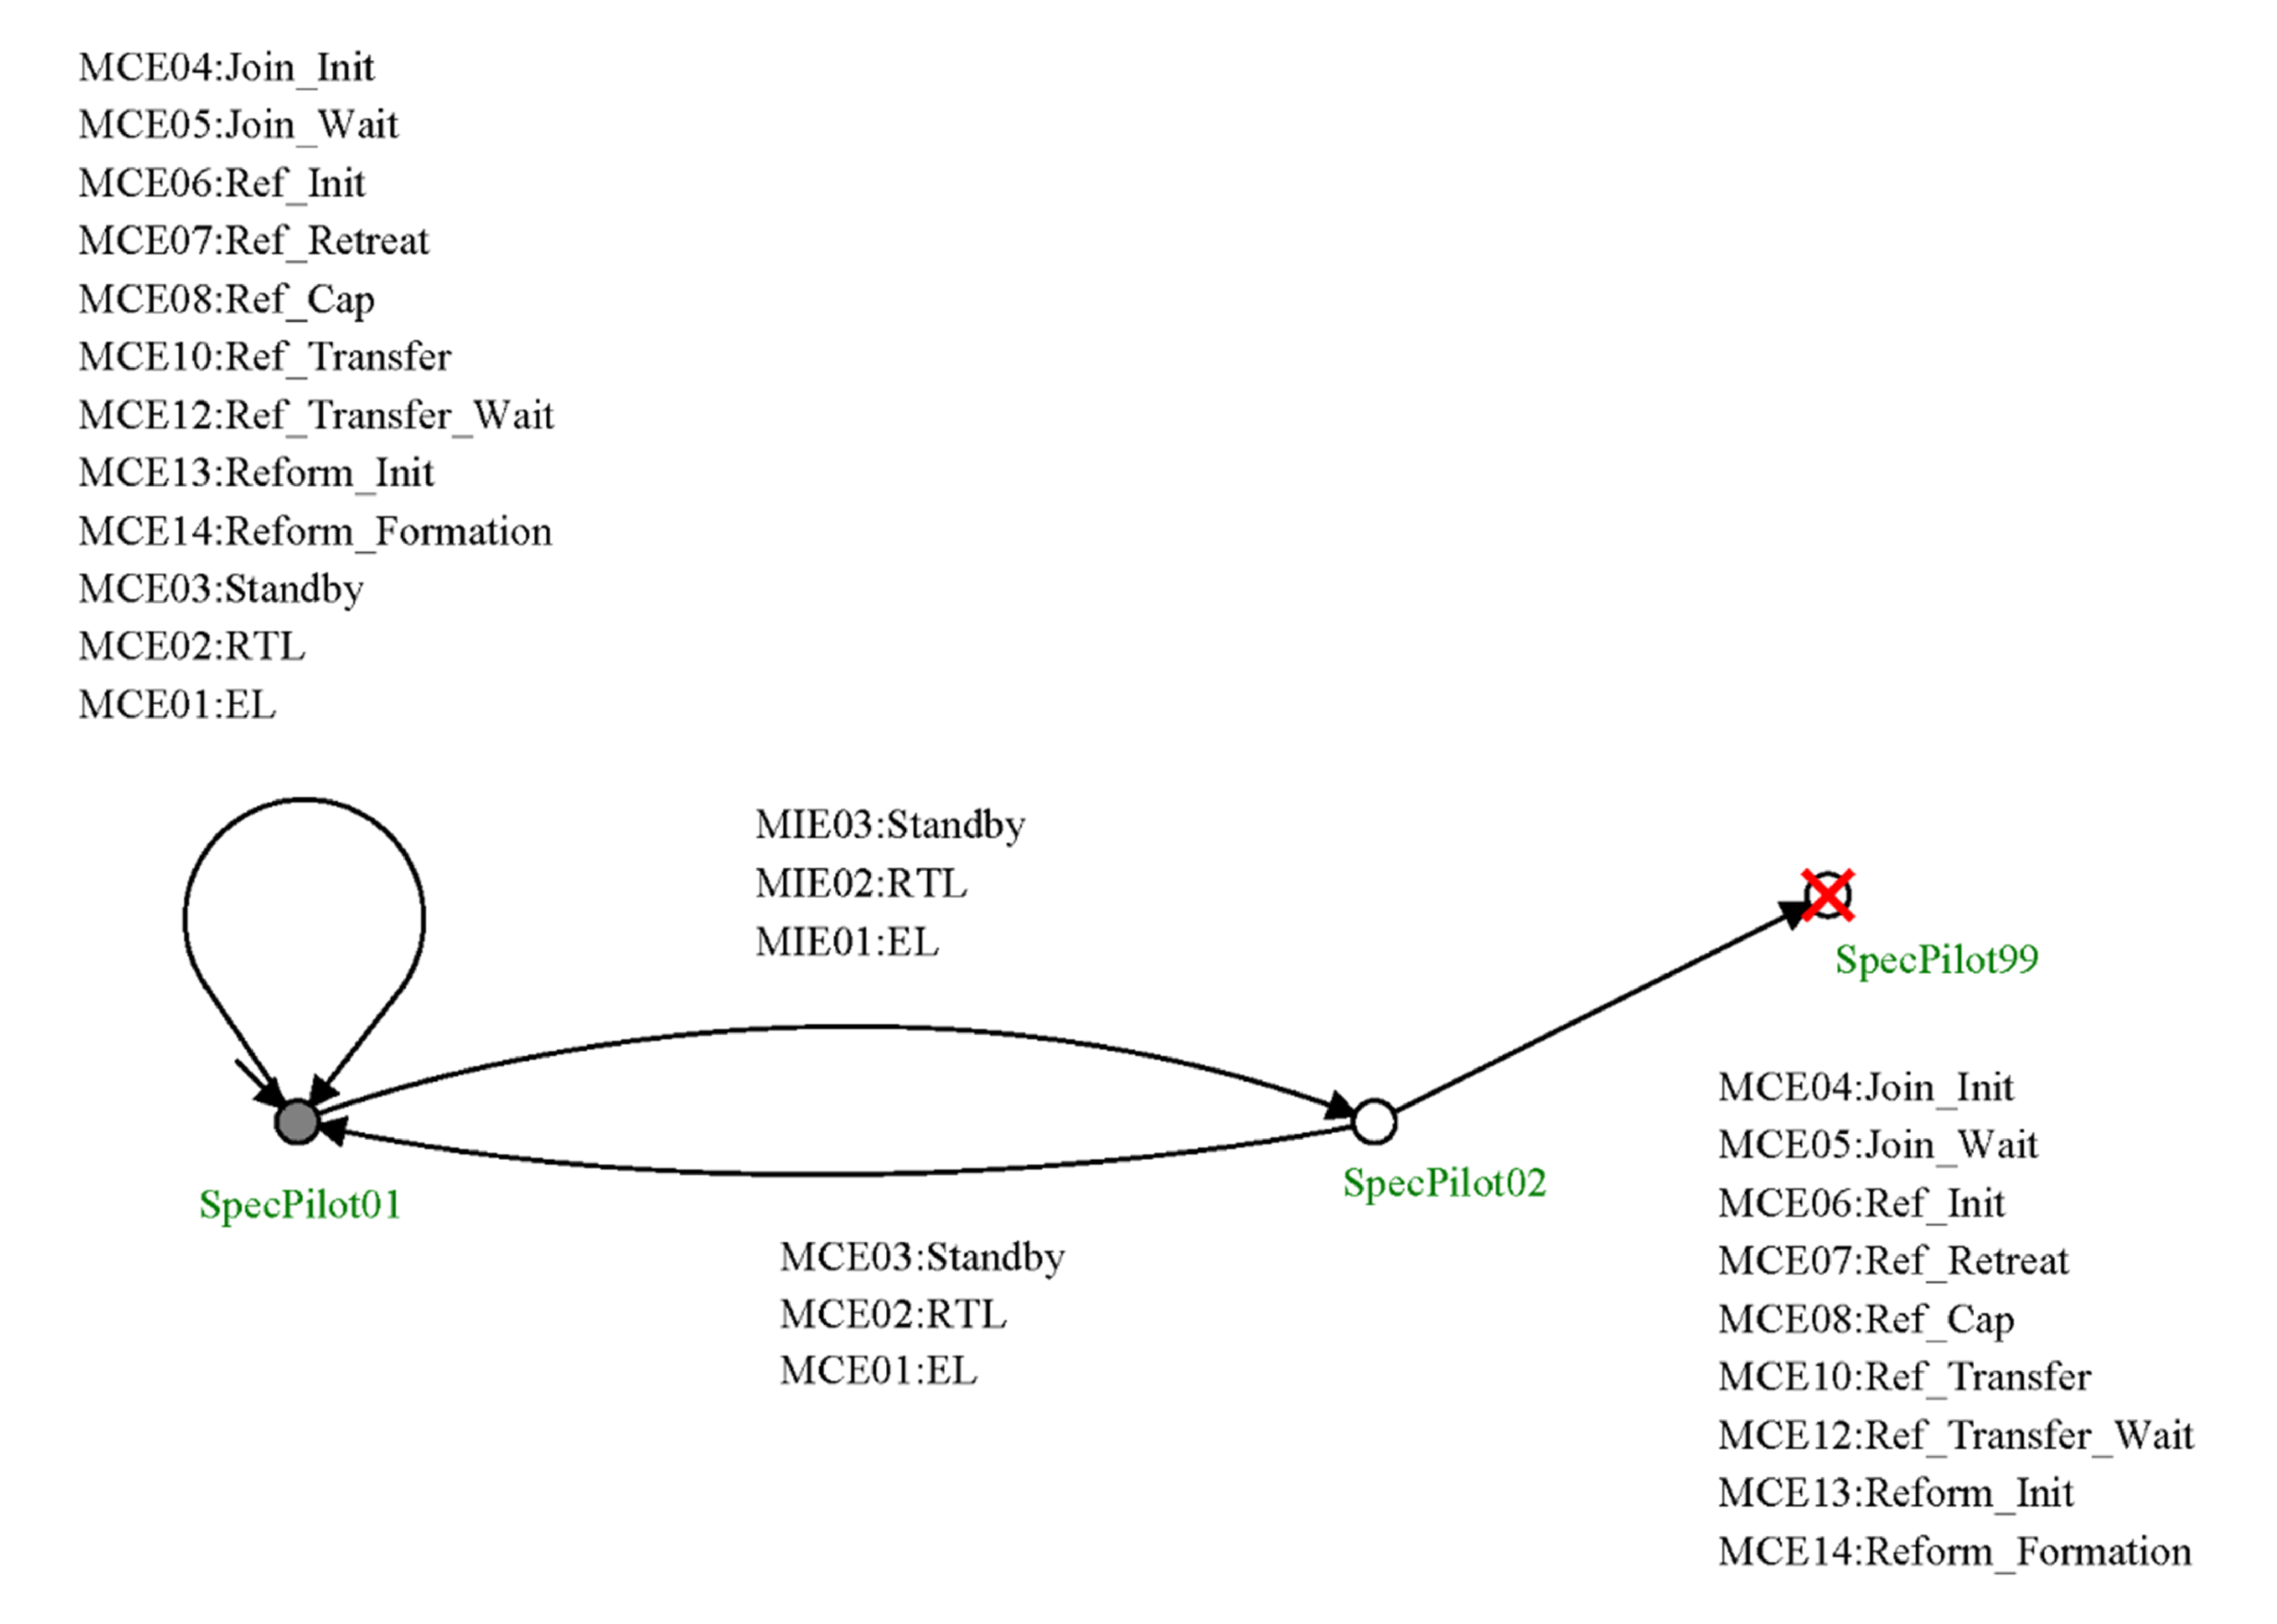
\includegraphics[width=0.9\textwidth]{Figures/Figs_Ch14/Fig21_HSPilot}
		\par\end{center}
	\caption{The holon of \textit{Spec-Pilot}.}
	\label{fig:specpilot} 
\end{figure}	


\subsection{Supervisor}
The \textit{Plant} provides the plant state, a 10-tuple representing the state of the whole system, while the \textit{Specification} points out the forbidden plant states. The supervisor is responsible for disabling certain controllable events (or enabling the rest) at certain plant states to guarantee that the \textit{Plant}  never reaches those forbidden plant states. The STSLib developed by [\citen{ma2008stslib}] is used to compute the supervisor of AAR, which finishes within 2 seconds on a personal laptop with 3.2GHZ I5 CPU and 8GB RAM. The supervisor is implemented in binary decision diagrams (BDD) for every MCE, and is converted into a lookup table including all plant states where the MCEs are allowed to happen. The converting program can be found in the supporting material. 

Take the resulting supervisor for MCE02 as an example. Its supervisor is shown in Table \ref{tab:mce02}, which shows eight different plant states where MCE02 is allowed to happen. That only \textit{Navigation}, \textit{Fuel} and \textit{Engine} are presented means that other superstates in the 10-tuple (such as \textit{Control, Datalink}) have no influence on the enablement of MCE02 and no need for checking as well. For example, plant state $ (Standby, Navigation01, \allowbreak Control01, Fuel01, Engine02, Drogue\\\&probe01, Datalink01, \allowbreak Tankersafety01,  Withdrawal01, Force01) $ satisfies the 2nd scenario in Table \ref{tab:mce02} and MCE02 is allowed to happen at this state.


\begin{table}
	\centering
	\caption{Supervisor for MCE02 in the form of  a lookup table}
	\label{tab:mce02}
	\begin{tabular}{c>{\hfil}p{60pt}<{\hfil}>{\hfil}p{40pt}<{\hfil}>{\hfil}p{40pt}<{\hfil}}
		\hline \hline
		Scenarios & Navigation & Fuel & Engine \\ \hline \hline
		1 & 1 & 1 & 1 \\ 
		2 & 1 & 1 & 2 \\ 
		3 & 1 & 2 & 1 \\ 
		4 & 1 & 2 & 2 \\ 
		5 & 2 & 1 & 1 \\ 
		6 & 2 & 1 & 2 \\ 
		7 & 2 & 2 & 1 \\
		8 & 2 & 2 & 2 \\ 
		\hline \hline
	\end{tabular}
\end{table}

Putting all these different lookup tables together and taking the union  of related superstates, the supervisor for the whole system can be presented in Table \ref{tab:supervisor}. Although the whole system has $ 413343 $ states in total, this table has only 235 rows, which shows the power of STS. Note that only 8 superstates need to be checked in the supervisor, fewer than the 10 superstates of plant states. The \textit{Autopilot} and \textit{Force} are ignored since there are no specific requirements about them in the specifications.

\begin{table*}[!htbp]
	\centering
	\caption{Supervisor in the form of a lookup table. Only part of the table is shown.\tnote{1}}
	\label{tab:supervisor}
	\begin{threeparttable}
		\begin{tabular}{|c|c|c|>{\hfil}p{30pt}<{\hfil}|>{\hfil}p{30pt}<{\hfil}|>{\hfil}p{30pt}<{\hfil}|>{\hfil}p{30pt}<{\hfil}|>{\hfil}p{30pt}<{\hfil}|c|}
			\hline
			\multirow{2}[5]{*}{Event} & \multirow{2}[5]{*}{Navigation} & \multirow{2}[5]{*}{Control\tnote{2}} & \multirow{2}[5]{*}{Fuel} & \multirow{2}[5]{*}{Engine} & \multirow{1}[5]{*}{Drogue} & \multirow{2}[-4]{*}{Datalink} & \multirow{1}[5]{*}{Tanker} & \multirow{2}[5]{*}{Withdrawal}\\
			& & & & & \multirow{1}[1]{*}{Probe} & & \multirow{1}[1]{*}{Safety} & \\ \hline
			MCE02 & 1 & 1$\sim$3 & 1 & 1 & 1$\sim$3 & 1$\sim$3 & 1$\sim$3 & 1$\sim$4 \\ \hline
			MCE02 & 1 & 1$\sim$3 & 1 & 3 & 1$\sim$3 & 1$\sim$3 & 1$\sim$3 & 1$\sim$4 \\ \hline
			\multicolumn{9}{|c|}{......} \\ \hline
			MCE07 & 1 & 1 & 1 & 1 & 1 & 1 & 1 & 1 \\ \hline
			MCE07 & 1 & 1 & 1 & 1 & 1 & 1 & 3 & 1 \\ \hline
			MCE07 & 1 & 1 & 1 & 1 & 1 & 3 & 1 & 1 \\ \hline
			MCE07 & 1 & 1 & 1 & 1 & 1 & 3 & 3 & 1 \\ \hline
			\multicolumn{9}{|c|}{......} \\ \hline
			MCE12 & 3 & 1 & 1 & 1 & 1 & 1 & 1 & 1 \\ \hline
			MCE12 & 3 & 1 & 1 & 1 & 1 & 1 & 3 & 1 \\ \hline
			MCE12 & 3 & 1 & 1 & 1 & 1 & 3 & 1 & 1 \\ \hline
			MCE12 & 3 & 1 & 1 & 1 & 1 & 3 & 3 & 1 \\ \hline
			\multicolumn{9}{|c|}{......} \\ \hline
			MCE14 & 3 & 3 & 1 & 3 & 1$\sim$3 & 1$\sim$3 & 1$\sim$3 & 1 \\ \hline
			MCE14 & 3 & 3 & 3 & 1 & 1$\sim$3 & 1$\sim$3 & 1$\sim$3 & 1 \\ \hline
			MCE14 & 3 & 3 & 3 & 3 & 1$\sim$3 & 1$\sim$3 & 1$\sim$3 & 1 \\ \hline
		\end{tabular}
		\begin{tablenotes}\footnotesize
			\item[1] In the implementation, states are represented by binary bits instead of decimal digits to improve program searching performance.
			\item[2] Here $ 1 \sim 3 $ means that \textit{Control} could be at \textit{Control01}, \textit{Control02} or \textit{Control03}. It is similar for other superstates.
		\end{tablenotes}
	\end{threeparttable}
\end{table*}

\section{Implementation and Simulation}
With the well-designed \textit{Plant} and obtained supervisor, this section presents the implementation architecture of applying such a logic controller to the autonomous receiver control system. Based on this, a simulation platform of AAR is built using MATLAB2016b to test  the logical correctness.

\subsection{Implementation architecture}
As shown in Fig. \ref{fig:implementation}, the logic controller should be put between low-level controllers and information sources including \textit{Sensor management}, \textit{Prognostics and Health Management} (PHM) \cite{kalgren2006defining} and \textit{Communication management}. The sensor management module is used to estimate the state of receivers such as location, velocity and altitude, determine what mode the receiver is currently in and then output the ATEs. For example, if this module confirms that the receiver has not arrived at the astern area (point $ C $ in Fig. \ref{fig:topview}), then ``ATE07:Ref-Init-Fail" is generated and output. The PHM module is used to detect subsystem failures and generate SFEs. The communication management is responsible for receiving pilot instructions and generating MIEs, e.g., when the pilot requires the receiver to return to land then "MIE02:RTL" is generated. The low-level controller is used to generate the direct control command for the receiver's velocity, acceleration, angular velocity, etc. There are 14 low-level controllers in correspondence to those 14 target modes such as STANDBY, JOINING-WAIT, and REFUELING-CAPTURE. At run time, the logic controller will choose one and only one low-level controller at the same time, i.e., only one MCE would be enabled.
\begin{figure}[h]
	\begin{center}
		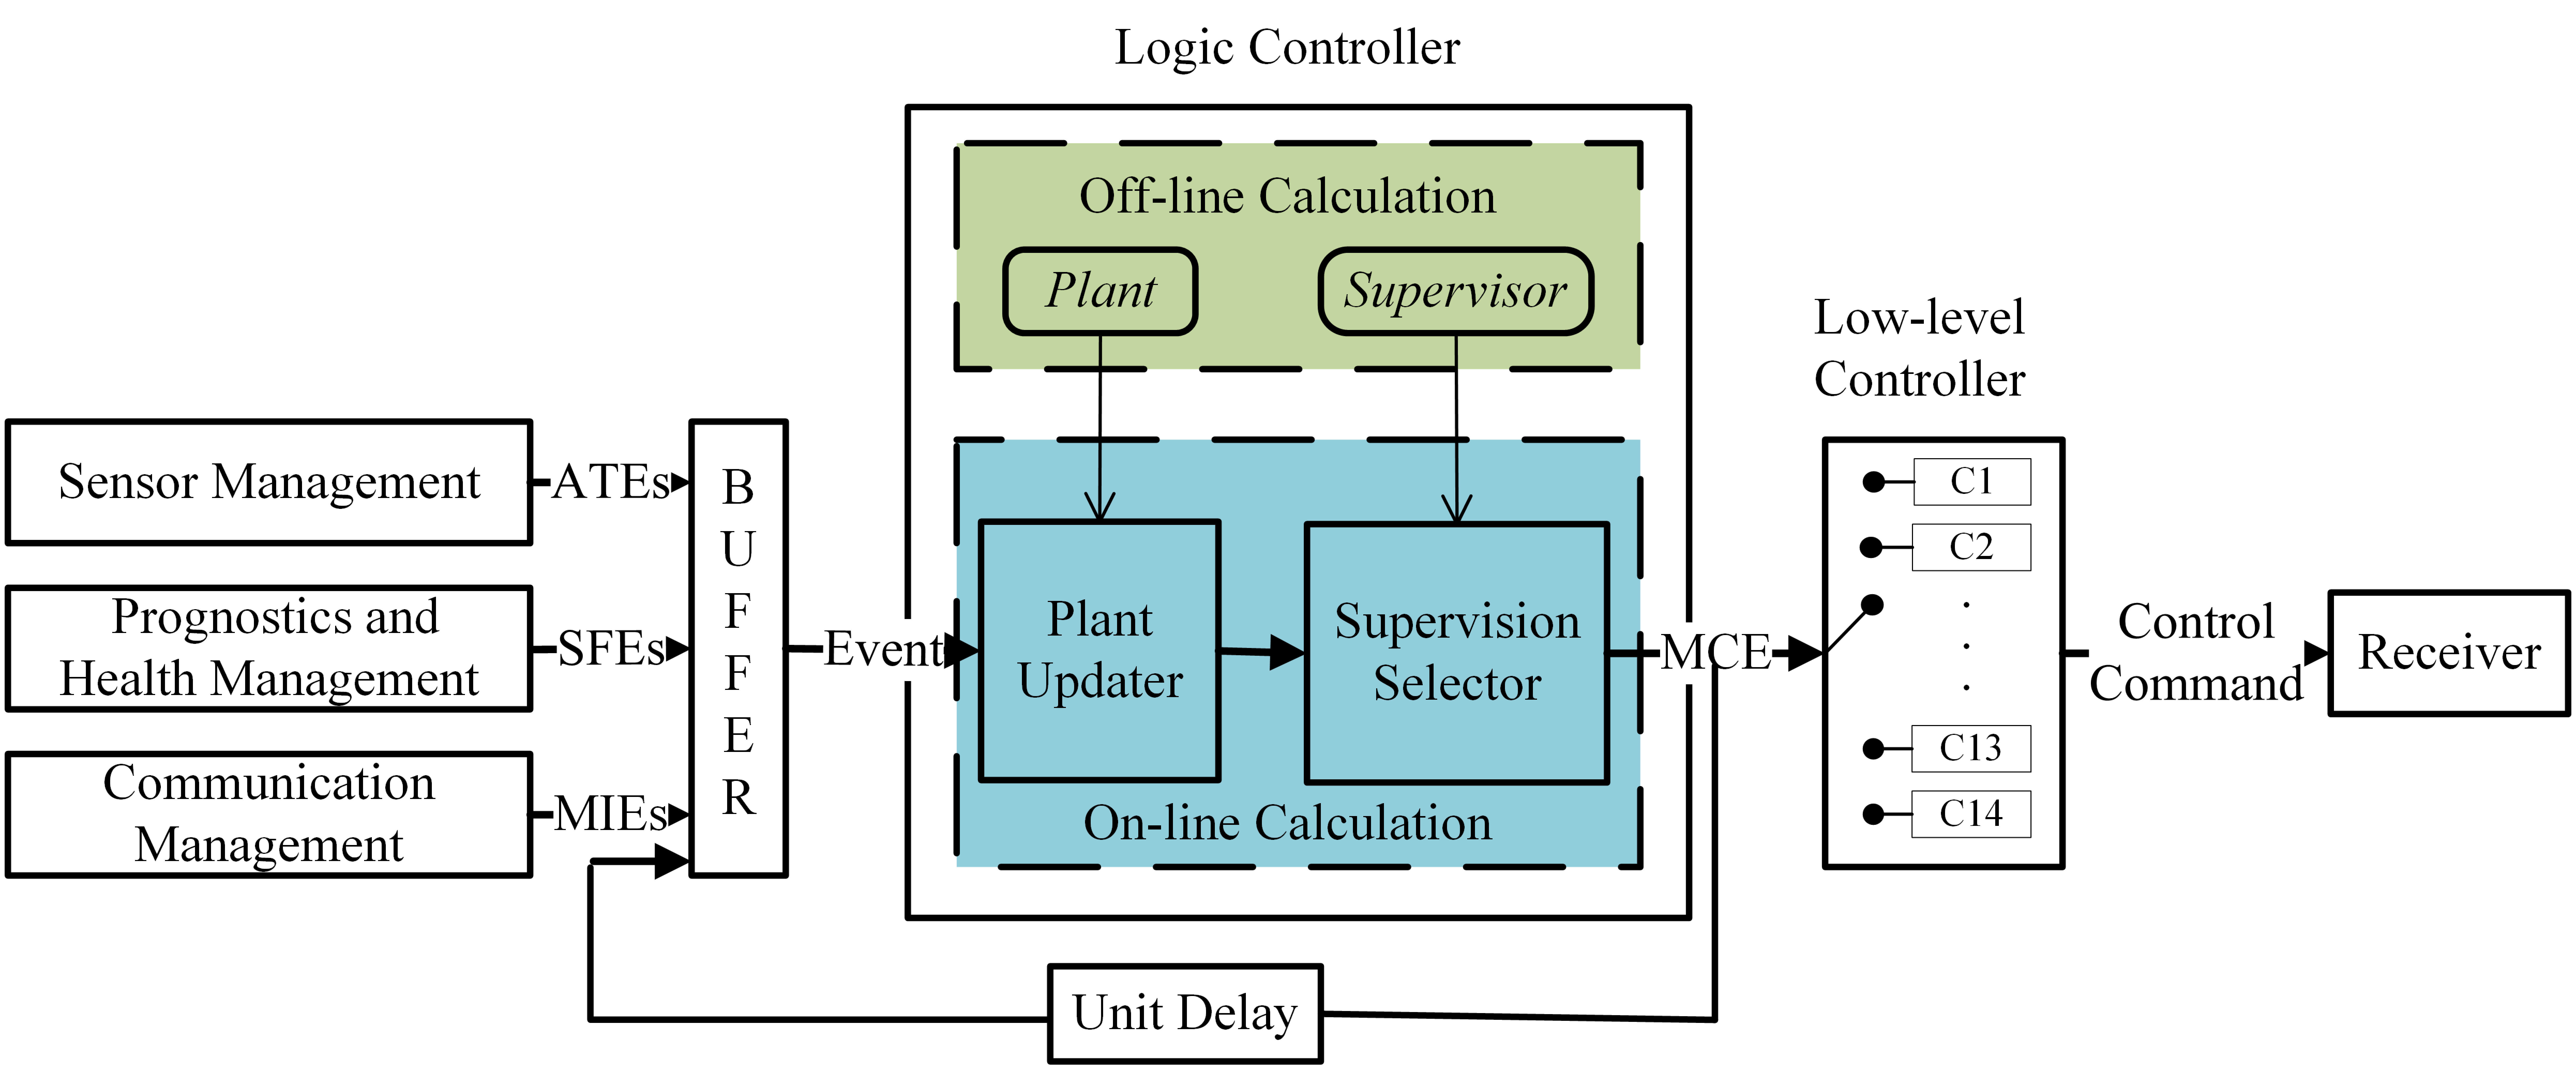
\includegraphics[width=0.9\textwidth]{Figures/Figs_Ch14/Fig22_ImpScheme}
		\par\end{center}
	\caption{The implementation Architecture.}
	\label{fig:implementation} 
\end{figure}	


The logic controller is divided into two parts: off-line and on-line. The \textit{Plant} (a holon or automaton with hierarchy structures) and \textit{Supervisor} (a loop-up table) can be computed off-line in advance and used as the input of on-line calculation. As for the on-line part, the \textit{Plant Updater} module receives events including ATEs, SFEs and MIEs from the corresponding source and then updates the current plant state according to the pre-defined \textit{Plant} holon. Note that the high-level decision-making is relatively slow in practice, but the low-level detection is fast. For example, the event ATEs, SFEs may be generated every 0.01s, but the decision period may be 1s. Thus a buffer is added to store those events according their occurrence sequence, and then to feed them all into the updater in every decision period. The \textit{Supervision Selector} would enable certain MCEs according to the current plant state and the pre-defined \textit{Supervisor}. The pseudo-code for the  procedure is shown in Table \ref{alg:decisionperiod} (The priority comparison presented in this algorithm is explained in the following Section \ref{sec:MCEPriority}).

\begin{table}
	\caption{Pseudo-code for on-line logic controller}
	\label{alg:decisionperiod}
	\begin{tabular}{p{15cm}}
		\hline \hline 
		On-line logic controller\\
		\hline \hline 
		$\mathbf{Input}$: the holon \textit{Plant}, the lookup table \textit{Supervisor}, initial \textit{Plant State} $ \mathbf{S}=\mathbf{S_0} $, $ \Delta $ is a positive integer representing a mode decision period, and a time counter $ k\in N $ and starts at 0, namely $ k=0 $.\\
		\textbf{Step 1}:  $ k = k + 1 $ \\
		\textbf{Step 2}: The sensor management, PHM and communication management detect the occurrence of ATEs, SFEs and MIEs. if $ k\ mod\ \Delta =0 $, go to Step 3; Otherwise, go to step 1.\\
		\textbf{Step 3}: Collect events occurring in the mode decision period $ \Delta $. \\
		\textbf{Step 4}: Update the plant state $ \mathbf{S} $ to $ \mathbf{S_1} $with events according to their occurrence sequence one by one. \\
		\textbf{Step 5}: Enable certain MCEs according to \textit{Supervisor} and current state $ \mathbf{S_1} $. Compare the priority of enabled MCEs and select one MCE with the highest priority. \\
		\textbf{Step 6}: Update the plant state $ \mathbf{S_1} $ to $ \mathbf{S_2} $ with the selected MCE. \\
		\textbf{Step 7}: $ \mathbf{S}=\mathbf{S_2} $, go to step 1. \\
		\hline \hline 
	\end{tabular}
\end{table}

\subsection{MCE Priority}
\label{sec:MCEPriority}
As mentioned before, the supervisor enforces the minimally restrictive behavior (set of generated event sequence) of plants under the restriction of specifications. Therefore, it will happen that several MCEs may be enabled at the same time and the same plant state. However, the aircraft can only be at one state, i.e., only one MCE can be picked and executed. Thus, the priority comparison among different MCEs is necessary for engineering practice. In this paper, the priority of MCEs is given according to their nodal distance to the success of AAR as defined in the flowchart shown in Fig. \ref{fig:priority}. And the priority is reflected by their indexes. That is to say, MCE01 possesses the least priority while MCE14 enjoys the highest priority.

For example, when the \textit{Plant} is at  state $(Refueling02, Navigation01, Control01, Fuel01, Engine01, \allowbreak Drogue\\\&probe01, Datalink01, Tankersafety01, Withdrawal01, \allowbreak Force01)$, MCE01,  MCE02, MCE03, and MCE08 are all enabled. But since  REFUELING-CAPTURE MODE is proceeding to the success of AAR but STANDBY, RTL and EL are proceeding to the failure of AAR. Therefore the event transiting to REFUELING-CAPTURE MODE is assigned with a higher priority than events transiting \allowbreak to  STANDBY, RTL and EL, and would be chosen in this state. 
\begin{figure}[h]
	\begin{center}
		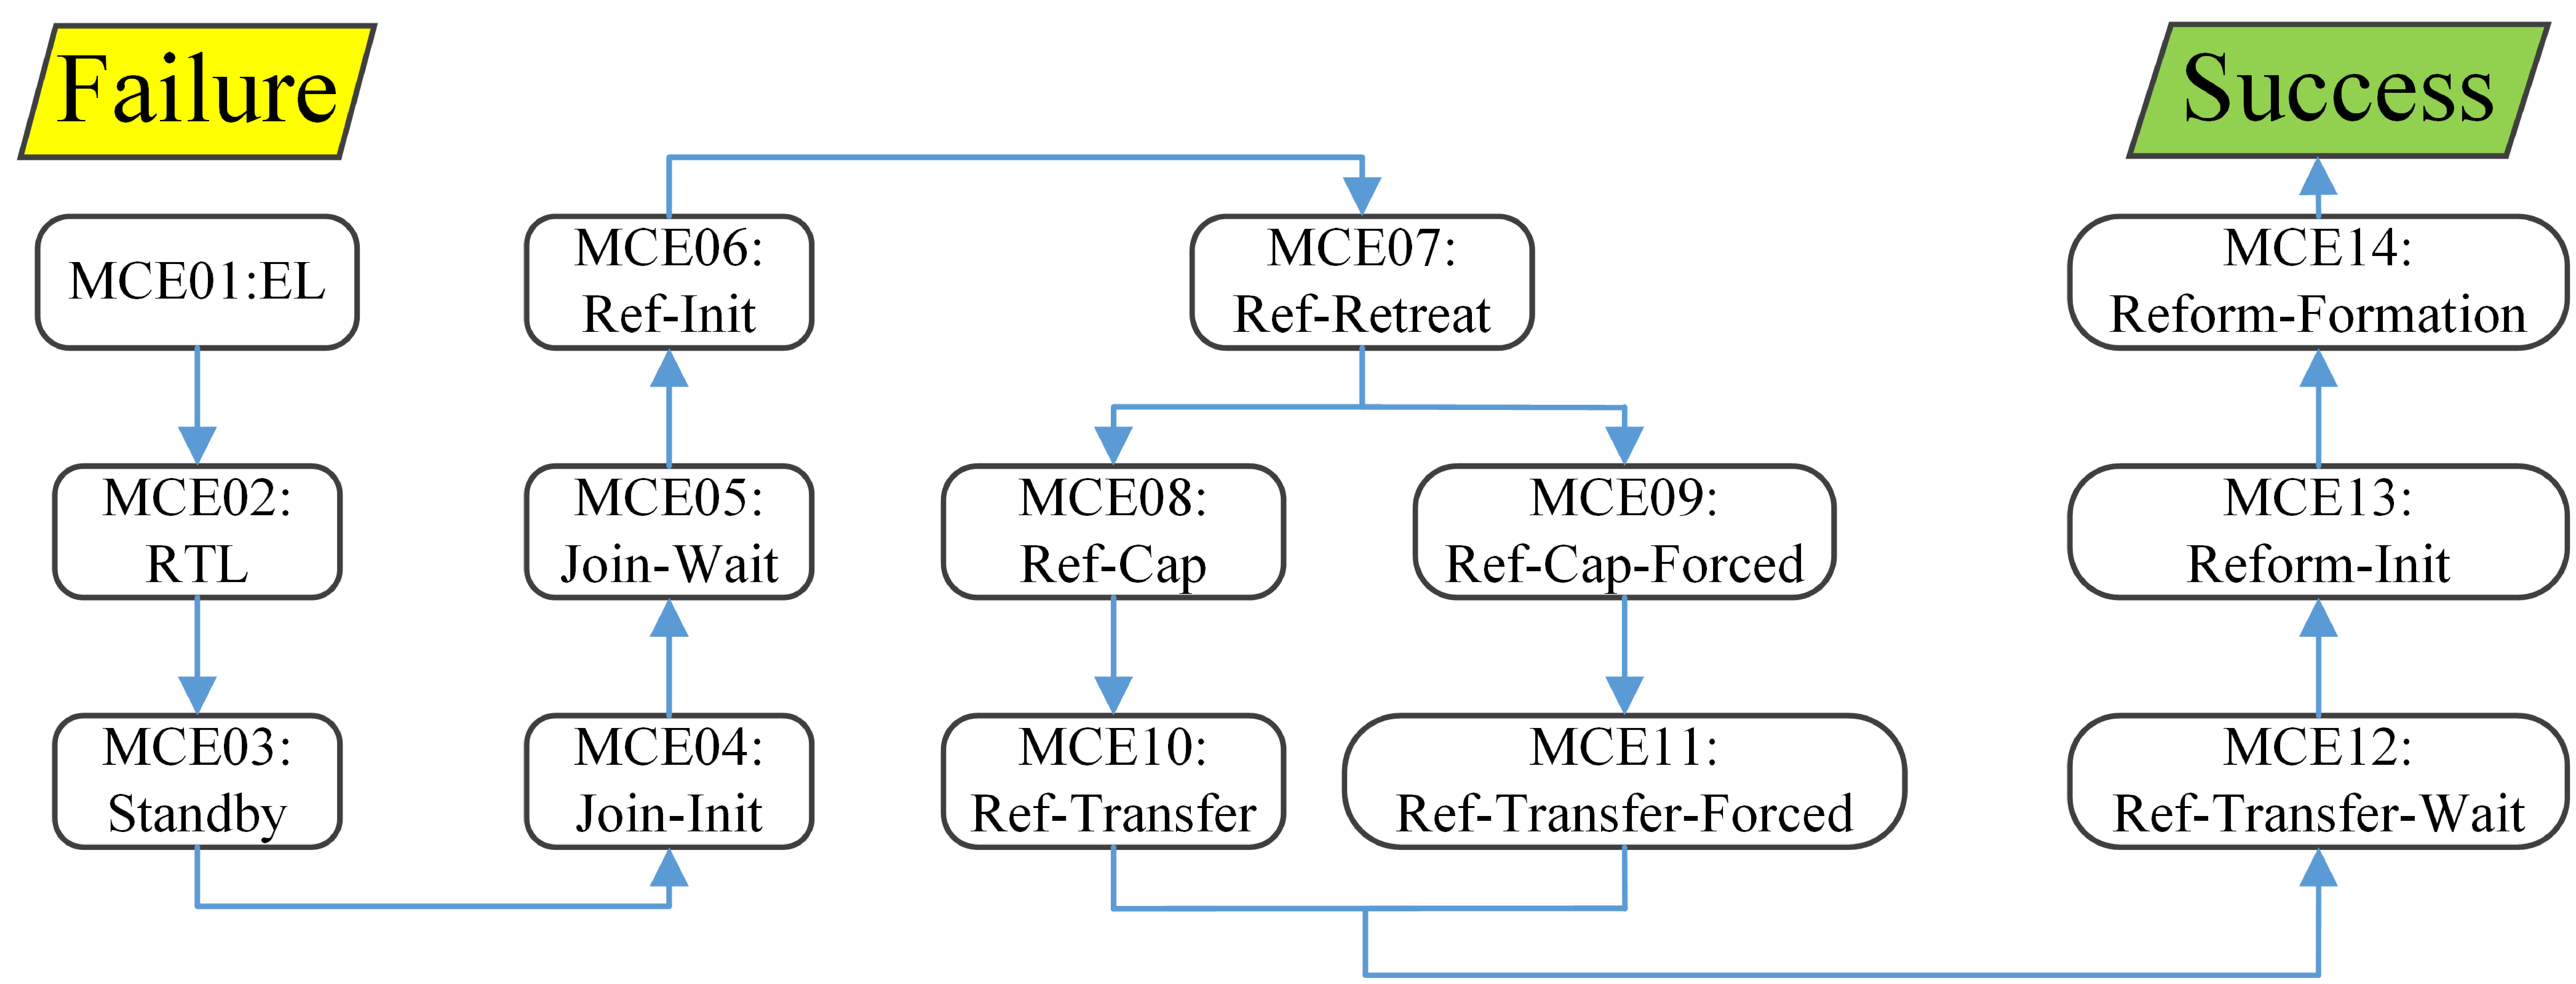
\includegraphics[width=0.7\textwidth]{Figures/Figs_Ch14/Fig23_Priority}
		\par\end{center}
	\caption{The flowchart of all MCEs in the AAR task. The distance of MCE is the  nodal distance between the MCE node and the "Success" node along the line.}
	\label{fig:priority} 
\end{figure}


\subsection{Simulation}
The simulation platform is built within MATLAB2016b according to the implementation architecture shown in Fig. \ref{fig:implementation}. This platform mainly consists of three parts: a Graphical User Interface (GUI), processing programs and a 3D visualization environment, as shown in Fig. \ref{fig:gui} and \ref{fig:vr}. The GUI enables the user to start, pause and terminate the simulation, input pilot commands (MIEs) and subsystem failures (SFEs)\footnote{The ATEs can be detected and generated automatically by the processing programs.}, and check the plant state and current MCE. The processing programs are the MATLAB functions used to implement the logic controller and low-level controller illustrated in Fig. \ref{fig:implementation}. In detail, the embedded dynamic models of Fighter-16 and Boeing-727 in MATLAB2016b are used to work as the receiver and the tanker.\footnote{For more detailed information about dynamic models and controller designs, please refer to \url{https://www.youtube.com/watch?v=spuXvSr31D8&feature=youtu.be}} Each low-level controller (in correspondence to each MCE) would give commands such as engine thrust, pitch angle, yaw angle to control the movement of the receiver. The 3D visualization environment presents the real-time state of the receiver, tanker, and the drogue-probe for a more direct observation.

Within this simulation platform, the user can add subsystem failures and pilot commands at any time. The failsafe mechanism or on-line logic controller will select out the best MCE according to the receiver's current health conditions and pre-defined safety requirements. The corresponding low-level controller will then control the movement of the receiver, which will be shown in the 3D simulation environment. This can enable the user to test the receiver's behavior under different possible situations. Three different testing scenarios are presented as follows, which cover the typical functional and safety requirements of AAR. Their textual descriptions are in Appendix \ref{app:test}, while videos can be found in \href{https://v.youku.com/v_show/id_XMzcwOTI0MDI4MA==.html?spm=a2h3j.8428770.3416059.1}{Youku} and \href{https://www.youtube.com/watch?v=PWLZffiGBoU&frags=pl\%2Cwn}{Youtube}
\footnote{For Youku, \url{https://youtu.be/R4-eMR9zqr0}. For Youtube, \url{ https://v.youku.com/v_show/id_XMzgwMTgwODU0OA==.html} }.
\begin{figure}[h]
	\begin{center}
		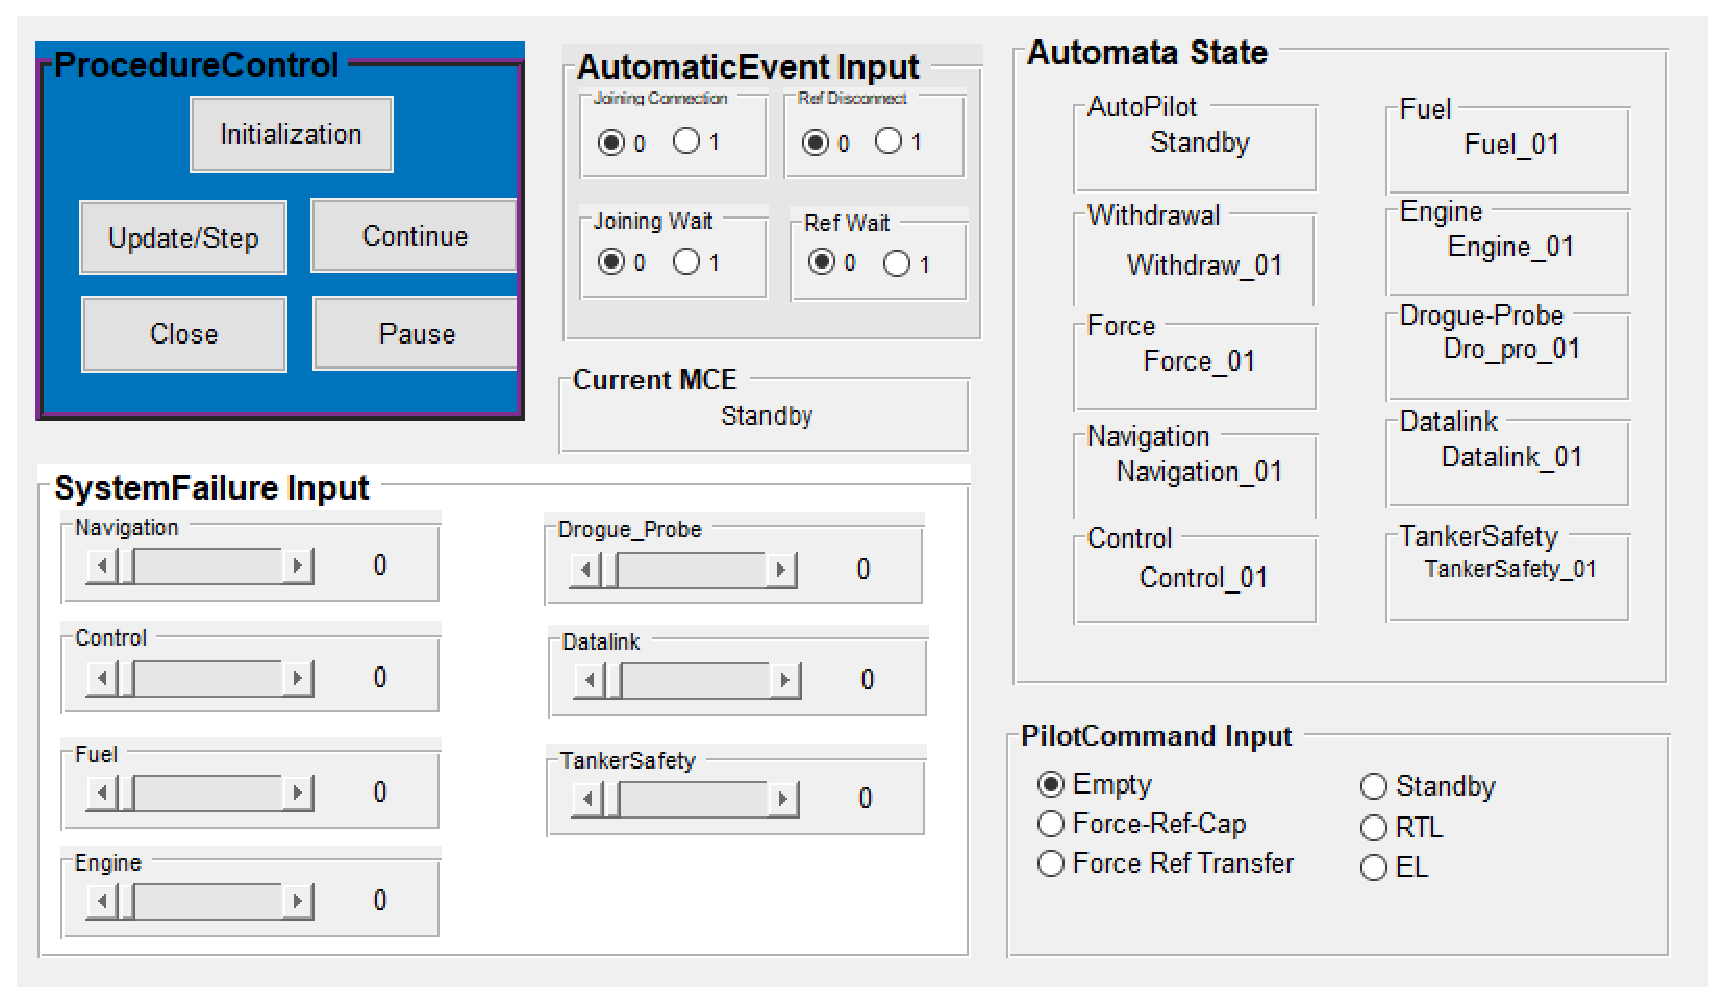
\includegraphics[width=0.8\textwidth]{Figures/Figs_Ch14/Fig24a_GUI}
		\par\end{center}
	\caption{raphical user interface.}
	\label{fig:gui} 
\end{figure}

\begin{figure}[h]
	\begin{center}
		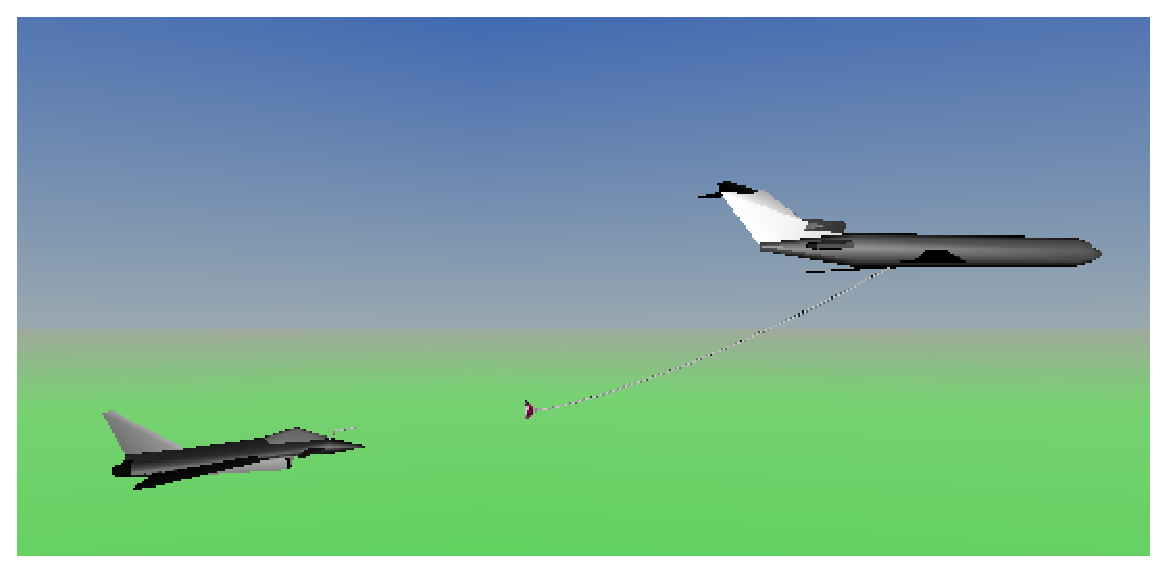
\includegraphics[width=0.8\textwidth]{Figures/Figs_Ch14/Fig24b_VR}
		\par\end{center}
	\caption{3D simulation environment.}
	\label{fig:vr} 
\end{figure}


\section{Chapter Summary}
This paper presents a new way to synthesize the failsafe mechanism of autonomous aerial refueling, namely the State Tree Structure. This formal method helps the system designer clarify all aspects of costumer's requirements at the early stage of product development. It can precisely define every detail of the logic control system, and thus achieve less ambiguity and more consistency compared with traditional document-based methods.

To apply this method to AAR, the continuous AAR procedure is first decomposed into ten discrete flight modes such as STANDBY, JOINING-INIT and REFUELING-CAPTURE MODE, and common safety issues of seven important subsystems like Navigation and Drogue \&Probe are collected. These describe the unrestricted behaviors of AAR, and thus define the plants of STS. Then, common user requirements including  seven functional demands and ten safety requirements are summarized. The functional demands emphasize what behaviors must be included in the system, so they are used to guide the design of plants. Since the safety requirements point out what behaviors are illegal, they define the specifications of STS. Finally, the software package STSLib is used to compute the supervisor. This final logic controller only has 235 rows, but controls a system with 413343 states.

Based on this, an implementation scheme is proposed and tested in a simulation environment built within MATLAB2016b. Three test cases are presented, recorded and proven to be error-free. Related tools and programs have been uploaded onto  \href{https://github.com/KevinDong0810/Failsafe-Design-for-AAR-using-STS}{Github}. The compact form of supervisor and the success of implementation reveals the power and great potential of supervisory control theory in the field of AAR. 





